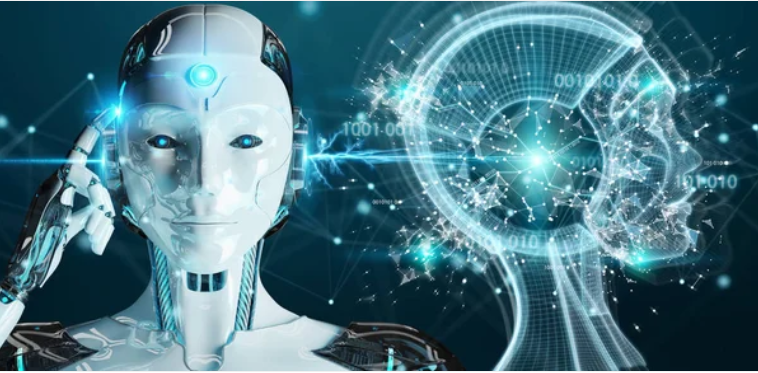
\includegraphics[width=8.49444in,height=4.14861in]{./images/image1.png}


\includegraphics[width=3.25903in,height=3.14722in]{./images/image3.png}

Cycle 3 : Modéliser et analyser les systèmes linéaires

\textbf{Modélisation des systèmes asservis}

Thomas Lusseau

Lycée Robert Doisneau - ATS

\hypertarget{table-des-matiuxe8res}{%
\section*{\texorpdfstring{\textbf{Table des matières}}{Table des matières}}\label{table-des-matiuxe8res}}
\addcontentsline{toc}{section}{\textbf{Table des matières}}

\protect\hyperlink{mise-en-situation}{1. MISE EN SITUATION \protect\hyperlink{mise-en-situation}{7}}

\protect\hyperlink{cas-n1-etuve-thermique}{1.1. Cas n°1~: Etuve thermique \protect\hyperlink{cas-n1-etuve-thermique}{7}}

\protect\hyperlink{cas-n2-toit-ouvrant-de-voiture}{1.2. Cas n°2~: Toit ouvrant de voiture \protect\hyperlink{cas-n2-toit-ouvrant-de-voiture}{8}}

\protect\hyperlink{introduction-aux-slci}{2. INTRODUCTION AUX SLCI \protect\hyperlink{introduction-aux-slci}{9}}

\protect\hyperlink{moduxe9lisation-de-connaissance}{3. Modélisation de connaissance \protect\hyperlink{moduxe9lisation-de-connaissance}{11}}

\protect\hyperlink{systuxe8mes-moduxe9lisables-par-un-gain}{3.1. Systèmes modélisables par un gain \protect\hyperlink{systuxe8mes-moduxe9lisables-par-un-gain}{11}}

\protect\hyperlink{non-linuxe9arituxe9-et-linuxe9arisation}{3.2. Non linéarité et linéarisation \protect\hyperlink{non-linuxe9arituxe9-et-linuxe9arisation}{14}}

\protect\hyperlink{transformuxe9e-de-laplace}{3.3. Transformée de Laplace \protect\hyperlink{transformuxe9e-de-laplace}{16}}

\protect\hyperlink{fonctions-de-transfert-cas-guxe9nuxe9rique}{3.4. Fonctions de transfert -- cas générique \protect\hyperlink{fonctions-de-transfert-cas-guxe9nuxe9rique}{23}}

\protect\hyperlink{forme-canonique-du-1er-ordre}{3.5. Forme canonique du 1\textsuperscript{er} ordre \protect\hyperlink{forme-canonique-du-1er-ordre}{25}}

\protect\hyperlink{fonctions-de-transfert-du-2d-ordre}{3.6. Fonctions de transfert du 2\textsuperscript{d} ordre \protect\hyperlink{fonctions-de-transfert-du-2d-ordre}{26}}

\protect\hyperlink{pruxe9voir-le-comportement-dun-systuxe8me-uxe0-partir-de-la-fonction-de-transfert}{4. Prévoir le comportement d'un système à partir de la fonction de transfert \protect\hyperlink{pruxe9voir-le-comportement-dun-systuxe8me-uxe0-partir-de-la-fonction-de-transfert}{29}}

\protect\hyperlink{pruxe9voir-le-comportement-en-stabilituxe9}{4.1. Prévoir le comportement en stabilité \protect\hyperlink{pruxe9voir-le-comportement-en-stabilituxe9}{29}}

\protect\hyperlink{pruxe9voir-le-comportement-en-rapidituxe9}{4.2. Prévoir le comportement en rapidité \protect\hyperlink{pruxe9voir-le-comportement-en-rapidituxe9}{31}}

\protect\hyperlink{pruxe9voir-le-comportement-en-pruxe9cision}{5. Prévoir le comportement en précision \protect\hyperlink{pruxe9voir-le-comportement-en-pruxe9cision}{32}}

\protect\hyperlink{_Toc99121097}{\textbf{6.} \textbf{Prévoir la réponse à un échelon} \protect\hyperlink{_Toc99121097}{33}}

\protect\hyperlink{_Toc99121098}{6.1. Modèle proportionnel \protect\hyperlink{_Toc99121098}{33}}

\protect\hyperlink{_Toc272938046}{6.2. Modèle intégrateur \protect\hyperlink{_Toc272938046}{33}}

\protect\hyperlink{_Toc379198200}{6.3. Réponse indicielle du 1\textsuperscript{er} ordre \protect\hyperlink{_Toc379198200}{33}}

\protect\hyperlink{_Toc99121102}{6.4. Réponse à une rampe du 1\textsuperscript{er} ordre \protect\hyperlink{_Toc99121102}{35}}

\protect\hyperlink{_Toc99121103}{6.5. Réponse du 2\textsuperscript{ème} ordre \protect\hyperlink{_Toc99121103}{36}}

\protect\hyperlink{identifier-un-moduxe8le-de-comportement}{7. Identifier un modèle de comportement \protect\hyperlink{identifier-un-moduxe8le-de-comportement}{41}}

\protect\hyperlink{muxe9thode-pour-identifier-un-moduxe8le-de-comportement}{7.1. Méthode pour identifier un modèle de comportement \protect\hyperlink{muxe9thode-pour-identifier-un-moduxe8le-de-comportement}{41}}

\protect\hyperlink{identification-temporelle-dun-1er-ordre}{7.2. Identification temporelle d'un 1er ordre \protect\hyperlink{identification-temporelle-dun-1er-ordre}{43}}

\protect\hyperlink{identification-temporelle-dun-2uxe8me-ordre-pseudo-puxe9riodique}{7.3. Identification temporelle d'un 2\textsuperscript{ème} ordre pseudo-périodique \protect\hyperlink{identification-temporelle-dun-2uxe8me-ordre-pseudo-puxe9riodique}{48}}

\protect\hyperlink{identification-temporelle-dun-2uxe8me-ordre-apuxe9riodique}{7.4. Identification temporelle d'un 2\textsuperscript{ème} ordre apériodique \protect\hyperlink{identification-temporelle-dun-2uxe8me-ordre-apuxe9riodique}{53}}

\protect\hyperlink{_Toc149497255}{7.5. Réduction de l'ordre d'un modèle \protect\hyperlink{_Toc149497255}{55}}

\protect\hyperlink{manipulation-des-blocs}{8. Manipulation des blocs \protect\hyperlink{manipulation-des-blocs}{58}}

\protect\hyperlink{eluxe9ments-de-bases}{8.1. Eléments de bases \protect\hyperlink{eluxe9ments-de-bases}{58}}

\protect\hyperlink{_Toc99121080}{\textbf{8.2.} \textbf{Chaîne directe et chaîne de retour} \protect\hyperlink{_Toc99121080}{58}}

\protect\hyperlink{_Toc149497259}{\textbf{8.3.} \textbf{Adaptateurs} \protect\hyperlink{_Toc149497259}{59}}

\protect\hyperlink{_Toc149497260}{\textbf{8.4.} \textbf{Quelques blocs classiques} \protect\hyperlink{_Toc149497260}{60}}

\protect\hyperlink{simplifier-un-schuxe9ma-bloc}{8.5. Simplifier un schéma-bloc \protect\hyperlink{simplifier-un-schuxe9ma-bloc}{61}}

\protect\hyperlink{schuxe9ma-bloc-uxe9quivalent}{8.1. Schéma-bloc équivalent \protect\hyperlink{schuxe9ma-bloc-uxe9quivalent}{69}}

\protect\hyperlink{systuxe8mes-asserivs-perturbuxe9s}{9. Systèmes asserivs perturbés \protect\hyperlink{systuxe8mes-asserivs-perturbuxe9s}{72}}

\protect\hyperlink{perturbation}{9.1. Perturbation \protect\hyperlink{perturbation}{72}}

\protect\hyperlink{schuxe9ma-bloc-dun-systuxe8me-perturbuxe9}{9.2. Schéma-bloc d'un système perturbé \protect\hyperlink{schuxe9ma-bloc-dun-systuxe8me-perturbuxe9}{73}}

\protect\hyperlink{thuxe9oruxe8me-de-superposition}{9.3. Théorème de superposition \protect\hyperlink{thuxe9oruxe8me-de-superposition}{73}}

\protect\hyperlink{stabilituxe9-dun-moduxe8le-perturbuxe9}{9.1. Stabilité d'un modèle perturbé \protect\hyperlink{stabilituxe9-dun-moduxe8le-perturbuxe9}{76}}

\protect\hyperlink{pruxe9cision-dun-moduxe8le-perturbuxe9}{9.2. Précision d'un modèle perturbé \protect\hyperlink{pruxe9cision-dun-moduxe8le-perturbuxe9}{76}}

\protect\hyperlink{erreur-statique-dun-systuxe8me-non-perturbuxe9}{9.3. Erreur statique d'un système non perturbé \protect\hyperlink{erreur-statique-dun-systuxe8me-non-perturbuxe9}{77}}

\protect\hyperlink{erreur-statique-due-uxe0-la-perturbation}{9.4. Erreur statique due à la perturbation \protect\hyperlink{erreur-statique-due-uxe0-la-perturbation}{80}}

\protect\hyperlink{rejet-de-perturbation}{9.5. Rejet de perturbation \protect\hyperlink{rejet-de-perturbation}{80}}

\protect\hyperlink{_Toc149497272}{\textbf{10.} \textbf{Analyse fréquentielle} \protect\hyperlink{_Toc149497272}{83}}

\protect\hyperlink{_Toc337686831}{\textbf{10.1.} \textbf{Caractéristiques} \protect\hyperlink{_Toc337686831}{83}}

\protect\hyperlink{_Toc272749600}{\textbf{10.2.} \textbf{Obtention de la réponse harmonique expérimentalement} \protect\hyperlink{_Toc272749600}{84}}

\protect\hyperlink{_Toc387521156}{\textbf{10.3.} \textbf{Fonction de transfert complexe} \protect\hyperlink{_Toc387521156}{85}}

\protect\hyperlink{lieux-de-transferts}{10.4. Lieux de transferts \protect\hyperlink{lieux-de-transferts}{86}}

\protect\hyperlink{duxe9cade-octave-duxe9cibel-propriuxe9tuxe9s-du-log10}{10.5. Décade, Octave, décibel, propriétés du log\textsubscript{10} \protect\hyperlink{duxe9cade-octave-duxe9cibel-propriuxe9tuxe9s-du-log10}{88}}

\protect\hyperlink{intuxe9ruxeat-de-luxe9chelle-logarithmique}{10.6. Intérêt de l'échelle logarithmique \protect\hyperlink{intuxe9ruxeat-de-luxe9chelle-logarithmique}{89}}

\protect\hyperlink{gain-et-phase}{10.7. Gain et phase \protect\hyperlink{gain-et-phase}{90}}

\protect\hyperlink{_Toc387521153}{\textbf{10.8.} \textbf{Définition du diagramme de Bode} \protect\hyperlink{_Toc387521153}{91}}

\protect\hyperlink{_Toc494227256}{\textbf{10.9.} \textbf{Filtre, pulsation de coupure et bande passante} \protect\hyperlink{_Toc494227256}{92}}

\protect\hyperlink{_Toc494227260}{\textbf{11.} \textbf{Réponse fréquentielle} \protect\hyperlink{_Toc494227260}{93}}

\protect\hyperlink{_Toc149497283}{\textbf{11.1.} \textbf{Modèle proportionnel} \protect\hyperlink{_Toc149497283}{93}}

\protect\hyperlink{_Toc337686846}{\textbf{11.2.} \textbf{Modèle intégrateur} \protect\hyperlink{_Toc337686846}{93}}

\protect\hyperlink{_Toc149497285}{\textbf{11.3.} \textbf{Modèle intégrateur de degré 2} \protect\hyperlink{_Toc149497285}{94}}

\protect\hyperlink{_Toc149497286}{\textbf{11.4.} \textbf{Modèle dérivateur} \protect\hyperlink{_Toc149497286}{94}}

\protect\hyperlink{_Toc99121126}{\textbf{11.5.} \textbf{Modèle du 1\textsuperscript{er} ordre} \protect\hyperlink{_Toc99121126}{94}}

\protect\hyperlink{_Toc494227268}{\textbf{11.6.} \textbf{Modèle du 1\textsuperscript{er} ordre inverse} \protect\hyperlink{_Toc494227268}{95}}

\protect\hyperlink{_Toc28847704}{\textbf{11.7.} \textbf{Méthode pour tracer les diagrammes de Bode} \protect\hyperlink{_Toc28847704}{99}}

\protect\hyperlink{_Toc99121133}{\textbf{11.8.} \textbf{Méthode pour tracer un diagramme de Bode} \protect\hyperlink{_Toc99121133}{99}}

\protect\hyperlink{_Toc149497291}{\textbf{11.9.} \textbf{Modèle du 2\textsuperscript{ème} ordre} \protect\hyperlink{_Toc149497291}{103}}

\protect\hyperlink{bilan-du-comportement-dun-moduxe8le-du-2uxe8me-ordre}{11.10. Bilan du comportement d'un modèle du 2ème ordre \protect\hyperlink{bilan-du-comportement-dun-moduxe8le-du-2uxe8me-ordre}{107}}

\protect\hyperlink{tracuxe9-de-bode-ruxe9el}{11.11. Tracé de Bode réel \protect\hyperlink{tracuxe9-de-bode-ruxe9el}{108}}

\protect\hyperlink{muxe9thode-pour-identifier-un-diagramme-de-bode}{11.1. Méthode pour identifier un diagramme de Bode \protect\hyperlink{muxe9thode-pour-identifier-un-diagramme-de-bode}{110}}

\protect\hyperlink{etude-de-la-stabilituxe9-point-critique}{12. Etude de la stabilité -- Point critique \protect\hyperlink{etude-de-la-stabilituxe9-point-critique}{116}}

\protect\hyperlink{_Toc59134857}{\textbf{12.1.} \textbf{Critère du revers dans le plan de Black -- hors programme} \protect\hyperlink{_Toc59134857}{117}}

\protect\hyperlink{_Toc59134858}{\textbf{12.2.} \textbf{Marge de phase et marge de gain des systèmes asservis} \protect\hyperlink{_Toc59134858}{118}}

\protect\hyperlink{performances-uxe0-uxe9tudier-en-ftbo-ou-en-ftbf}{12.3. Performances à étudier en FTBO ou en FTBF \protect\hyperlink{performances-uxe0-uxe9tudier-en-ftbo-ou-en-ftbf}{123}}

\protect\hyperlink{sources}{13. Sources \protect\hyperlink{sources}{123}}

\protect\hyperlink{questions-de-cours}{14. QUESTIONS DE COURS \protect\hyperlink{questions-de-cours}{123}}

Donner les démarches et outils nécessaires à la modélisation et à l'étude des systèmes asservis.

\textbf{Je connais~:}

\begin{longtable}[]{@{}
  >{\raggedright\arraybackslash}p{(\columnwidth - 2\tabcolsep) * \real{0.9045}}
  >{\raggedright\arraybackslash}p{(\columnwidth - 2\tabcolsep) * \real{0.0955}}@{}}
\toprule\noalign{}
\begin{minipage}[b]{\linewidth}\raggedright
\begin{itemize}
\item
  les propriétés d'un SLCI~;
\end{itemize}
\end{minipage} & \begin{minipage}[b]{\linewidth}\raggedright
⃝
\end{minipage} \\
\midrule\noalign{}
\endhead
\bottomrule\noalign{}
\endlastfoot
\begin{minipage}[t]{\linewidth}\raggedright
\begin{itemize}
\item
  les différents types de non linéarités~;
\end{itemize}
\end{minipage} & ⃝ \\
\begin{minipage}[t]{\linewidth}\raggedright
\begin{itemize}
\item
  les propriétés (dérivation, intégration, linéarité) et les théorèmes (valeurs finale et initiale, retard) de la Transformée de Laplace~;
\end{itemize}
\end{minipage} & ⃝ \\
\begin{minipage}[t]{\linewidth}\raggedright
\begin{itemize}
\item
  les Transformées de Laplace usuelles (échelon, rampe)~;
\end{itemize}
\end{minipage} & ⃝ \\
\begin{minipage}[t]{\linewidth}\raggedright
\begin{itemize}
\item
  les formes canoniques des fonctions de transfert du premier et deuxième ordre ~;~
\end{itemize}
\end{minipage} & ⃝ \\
\begin{minipage}[t]{\linewidth}\raggedright
\begin{itemize}
\item
  les règles de simplifications des schéma-blocs~;
\end{itemize}
\end{minipage} & ⃝ \\
\begin{minipage}[t]{\linewidth}\raggedright
\begin{itemize}
\item
  la FTBO et la FTBF~;
\end{itemize}
\end{minipage} & ⃝ \\
\begin{minipage}[t]{\linewidth}\raggedright
\begin{itemize}
\item
  les caractéristiques des réponses indicielles du 1\textsuperscript{er} et 2\textsuperscript{ème} ordre~;
\end{itemize}
\end{minipage} & ⃝ \\
\begin{minipage}[t]{\linewidth}\raggedright
\begin{itemize}
\item
  la méthode pour trouver la transformée inverse de Laplace~;
\end{itemize}
\end{minipage} & ⃝ \\
\begin{minipage}[t]{\linewidth}\raggedright
\begin{itemize}
\item
  les caractéristiques principales d'une sinusoïde~;
\end{itemize}
\end{minipage} & ⃝ \\
\begin{minipage}[t]{\linewidth}\raggedright
\begin{itemize}
\item
  la définition des diagrammes de Bode (gain et de phase)~;
\end{itemize}
\end{minipage} & ⃝ \\
\begin{minipage}[t]{\linewidth}\raggedright
\begin{itemize}
\item
  les valeurs et les propriétés importantes du log\textsubscript{10}~;
\end{itemize}
\end{minipage} & ⃝ \\
\begin{minipage}[t]{\linewidth}\raggedright
\begin{itemize}
\item
  les termes~: décade, octave et la définition du décibel~;
\end{itemize}
\end{minipage} & ⃝ \\
\begin{minipage}[t]{\linewidth}\raggedright
\begin{itemize}
\item
  les fonctions de transferts élémentaires et leurs diagrammes de Bode asymptotiques et réels~;
\end{itemize}
\end{minipage} & ⃝ \\
\begin{minipage}[t]{\linewidth}\raggedright
\begin{itemize}
\item
  la méthode pour tracer les diagrammes de Bode~;
\end{itemize}
\end{minipage} & ⃝ \\
\begin{minipage}[t]{\linewidth}\raggedright
\begin{itemize}
\item
  la définition de la bande passante à -3dB~;
\end{itemize}
\end{minipage} & ⃝ \\
\begin{minipage}[t]{\linewidth}\raggedright
\begin{itemize}
\item
  le facteur de résonance et l'incidence de l'amortissement sur les diagrammes de Bode d'une fonction du 2\textsuperscript{ème} ordre.
\end{itemize}
\end{minipage} & ⃝ \\
\begin{minipage}[t]{\linewidth}\raggedright
\begin{itemize}
\item
  les définitions des marges de phase et de gain et le critère de stabilité.
\end{itemize}
\end{minipage} & ⃝ \\
\end{longtable}

\textbf{Je sais~:}

\begin{longtable}[]{@{}
  >{\raggedright\arraybackslash}p{(\columnwidth - 6\tabcolsep) * \real{0.8904}}
  >{\raggedright\arraybackslash}p{(\columnwidth - 6\tabcolsep) * \real{0.0140}}
  >{\raggedright\arraybackslash}p{(\columnwidth - 6\tabcolsep) * \real{0.0803}}
  >{\raggedright\arraybackslash}p{(\columnwidth - 6\tabcolsep) * \real{0.0152}}@{}}
\toprule\noalign{}
\begin{minipage}[b]{\linewidth}\raggedright
\begin{itemize}
\item
  linéariser une fonction de transfert non linéaire autour d'un point de fonctionnement~;
\end{itemize}
\end{minipage} & \multicolumn{2}{>{\raggedright\arraybackslash}p{(\columnwidth - 6\tabcolsep) * \real{0.0944} + 2\tabcolsep}}{%
\begin{minipage}[b]{\linewidth}\raggedright
⃝
\end{minipage}} & \begin{minipage}[b]{\linewidth}\raggedright
\end{minipage} \\
\midrule\noalign{}
\endhead
\bottomrule\noalign{}
\endlastfoot
\begin{minipage}[t]{\linewidth}\raggedright
\begin{itemize}
\item
  déterminer le modèle de constituants modélisables par un gain (ressort, \ldots)~
\end{itemize}
\end{minipage} & \multicolumn{2}{>{\raggedright\arraybackslash}p{(\columnwidth - 6\tabcolsep) * \real{0.0944} + 2\tabcolsep}}{%
⃝} & \\
\begin{minipage}[t]{\linewidth}\raggedright
\begin{itemize}
\item
  transformer une équation différentielle dans le domaine de Laplace~;
\end{itemize}
\end{minipage} & \multicolumn{2}{>{\raggedright\arraybackslash}p{(\columnwidth - 6\tabcolsep) * \real{0.0944} + 2\tabcolsep}}{%
⃝} & \\
\begin{minipage}[t]{\linewidth}\raggedright
\begin{itemize}
\item
  trouver la forme canonique des fonctions de transfert du premier et deuxième ordre~;~
\end{itemize}
\end{minipage} & \multicolumn{2}{>{\raggedright\arraybackslash}p{(\columnwidth - 6\tabcolsep) * \real{0.0944} + 2\tabcolsep}}{%
⃝} & \\
\begin{minipage}[t]{\linewidth}\raggedright
\begin{itemize}
\item
  simplifier un schéma-bloc~;~
\end{itemize}
\end{minipage} & \multicolumn{2}{>{\raggedright\arraybackslash}p{(\columnwidth - 6\tabcolsep) * \real{0.0944} + 2\tabcolsep}}{%
⃝} & \\
\begin{minipage}[t]{\linewidth}\raggedright
\begin{itemize}
\item
  déterminer les fonctions de transfert en boucle ouverte et en boucle fermée d\textquotesingle un système à partir de la connaissance des fonctions de transfert le constituant
\end{itemize}
\end{minipage} & \multicolumn{2}{>{\raggedright\arraybackslash}p{(\columnwidth - 6\tabcolsep) * \real{0.0944} + 2\tabcolsep}}{%
⃝} & \\
\begin{minipage}[t]{\linewidth}\raggedright
\begin{itemize}
\item
  tracer les~allures des réponses indicielles des fonctions de transfert du 1\textsuperscript{er} et 2\textsuperscript{ème} ordre~;
\end{itemize}
\end{minipage} & \multicolumn{2}{>{\raggedright\arraybackslash}p{(\columnwidth - 6\tabcolsep) * \real{0.0944} + 2\tabcolsep}}{%
⃝} & \\
\begin{minipage}[t]{\linewidth}\raggedright
\begin{itemize}
\item
  trouver la Transformée inverse de Laplace d'une fonction de transfert~;~
\end{itemize}
\end{minipage} & \multicolumn{2}{>{\raggedright\arraybackslash}p{(\columnwidth - 6\tabcolsep) * \real{0.0944} + 2\tabcolsep}}{%
⃝} & \\
\begin{minipage}[t]{\linewidth}\raggedright
\begin{itemize}
\item
  tracer les diagrammes de Bode de n'importe quelle fonction de transfert~;
\end{itemize}
\end{minipage} & \multicolumn{2}{>{\raggedright\arraybackslash}p{(\columnwidth - 6\tabcolsep) * \real{0.0944} + 2\tabcolsep}}{%
⃝} & \\
\begin{minipage}[t]{\linewidth}\raggedright
\begin{itemize}
\item
  trouver la bande passante à -3 dB à partir du diagramme de gain d'une fonction de transfert~;
\end{itemize}
\end{minipage} & \multicolumn{2}{>{\raggedright\arraybackslash}p{(\columnwidth - 6\tabcolsep) * \real{0.0944} + 2\tabcolsep}}{%
⃝} & \\
\begin{minipage}[t]{\linewidth}\raggedright
\begin{itemize}
\item
  déterminer les marges de phase et de gain d'un système puis analyser la stabilité d'un système en boucle fermée.
\end{itemize}
\end{minipage} & \multicolumn{2}{>{\raggedright\arraybackslash}p{(\columnwidth - 6\tabcolsep) * \real{0.0944} + 2\tabcolsep}}{%
⃝} & \\
\multicolumn{2}{@{}>{\raggedright\arraybackslash}p{(\columnwidth - 6\tabcolsep) * \real{0.9045} + 2\tabcolsep}}{%
\begin{minipage}[t]{\linewidth}\raggedright
\begin{itemize}
\item
  identifier un système à partir d\textquotesingle une courbe de réponse indicielle ou d'une réponse harmonique et donner un modèle de représentation.
\end{itemize}
\end{minipage}} & \multicolumn{2}{>{\raggedright\arraybackslash}p{(\columnwidth - 6\tabcolsep) * \real{0.0955} + 2\tabcolsep}@{}}{%
⃝} \\
\end{longtable}

\hypertarget{mise-en-situation}{%
\subsection{MISE EN SITUATION}\label{mise-en-situation}}

\hypertarget{cas-n1-etuve-thermique}{%
\subsubsection[Cas n°1~: Etuve thermique]{\texorpdfstring{\protect
\includegraphics[width=1.41875in,height=1.4in]{./images/image5.png}Cas n°1~: Etuve thermique}{Cas n°1~: Etuve thermique}}\label{cas-n1-etuve-thermique}}

L'étuve thermique est utilisée pour la stérilisation des ustensiles de laboratoire (tubes à essai, boîtes de Pétri, tubes à culture et bouchons, pipettes Pasteur et récipients divers). Elle permet un réglage de température de la température ambiante jusqu\textquotesingle à 200 °C.

Pour supprimer les micro-organismes, il est nécessaire de chauffer pendant 2 heures à une température constante de 150°C .


\includegraphics[width=3.725in,height=2.50208in]{./images/image6.png}Une résistance électrique alimentée par une tension \(U(t)\) assure le chauffage à l\textquotesingle intérieur de l\textquotesingle étuve. Une sonde de température Pt100, associée à un conditionneur permet de mesurer la température \(\theta(t)\) dans l\textquotesingle étuve.

La tension de commande u\textsubscript{c}(t) est construite de la façon suivante : u\textsubscript{c}(t) = K.ε(t) et ε(t) = u\textsubscript{e}(t)--u\textsubscript{m}(t) avec K égal à 20.

u\textsubscript{e}(t) étant la tension de consigne de l\textquotesingle asservissement et u\textsubscript{m}(t) la tension de mesure fournie par le conditionneur du capteur de température.

\textbf{Comment déterminer le modèle mathématique des différents blocs afin d'optimiser la régulation de température~?}

\hypertarget{cas-n2-toit-ouvrant-de-voiture}{%
\subsubsection{Cas n°2~: Toit ouvrant de voiture}\label{cas-n2-toit-ouvrant-de-voiture}}

\begin{quote}

\includegraphics[width=1.82986in,height=0.75in]{./images/image8.jpeg}Le toit ouvrant est un sous-système du véhicule automobile qui permet une meilleure ventilation de l'habitacle et procure aux passagers des sensations de liberté et une meilleure luminosité. L'ensemble est alimenté par la batterie du véhicule dont la tension est notée \textbf{U\textsubscript{b} = 13 V}.

La chaîne d'énergie comprend, comme composant principal, un bloc dénommé \textbf{moto - réducteur}, composé d'un moteur à courant continu à aimants permanents et d'un \textbf{réducteur mécanique à roue et vis sans fin} dont les caractéristiques sont~:
\end{quote}

\begin{itemize}
\item
  Vis à 2 filets équivalent à \textbf{Z\textsubscript{v} = 2 dents}
\item
  Roue du réducteur à \textbf{Z\textsubscript{r} = 55 dents}
\end{itemize}

\begin{quote}
Le diamètre primitif du pignon de sortie du réducteur est \textbf{D = 16 mm}. Il engrène sur \textbf{deux crémaillères souples} (droite et gauche), sur lesquelles sont fixés \textbf{deux chariots droit et gauche}, permettant de mettre en mouvement le toit ouvrant.

La mise en position du toit nécessite l'emploi de boucles d'asservissement dont le schéma fonctionnel est donné ci-dessous~:


\includegraphics[width=6.89792in,height=2.12014in]{./images/image9.png}
\end{quote}

\textbf{Comment déterminer le modèle mathématique des différents blocs afin d'optimiser les performances du déplacement du toit ouvrant~?}


\includegraphics[width=4.61667in,height=1.82847in]{./images/image10.png}

\hypertarget{introduction-aux-slci}{%
\subsection{INTRODUCTION AUX SLCI}\label{introduction-aux-slci}}

Pour \textbf{évaluer (et/ou améliorer) les performances} (rapidité, précision, stabilité, dépassement) des systèmes asservis, il faut connaître le modèle notre système et lui appliquer les signaux ``tests''. Cela peut être sur le système réel ou en simulation. Pour déterminer ces modèles et réaliser des simulations, il existe la théorie des \textbf{SLCI (Systèmes Linéaires Continus Invariants).}

\hypertarget{section}{%
\subparagraph*{}\label{section}}
\addcontentsline{toc}{subparagraph}{}

\hypertarget{hypothuxe8ses-et-duxe9finitions}{%
\subparagraph*{Hypothèses et Définitions}\label{hypothuxe8ses-et-duxe9finitions}}
\addcontentsline{toc}{subparagraph}{Hypothèses et Définitions}

Un \textbf{SLCI} (\textbf{Système Linéaire, Continu et Invariant~}) est un système (ou un constituant du système) dont la relation entre la grandeur d'entrée e(t) et la grandeur sortie s(t) est une \textbf{équation différentielle linéaires à coefficients constants} de la forme~:

\(a_{n}\frac{d^{n}s}{{dt}^{n}}(t) + \ldots + a_{1}\frac{ds}{dt}(t) + a_{0}s(t) = b_{m}\frac{d^{m}e}{{dt}^{m}}(t) + \ldots + b_{1}\frac{de}{dt}(t) + b_{0}e(t)\)

\(e(t):entrée\ \ \ \ \ \ et\ \ \ \ \ \ s(t):sortie\)

\textbf{\emph{n}} est l\textquotesingle{}\textbf{ordre} du modèle. C'est le degré de l'équation différentielle.

Pour des raisons liées à la \textbf{causalité} (le comportement d\textquotesingle un système dépend du passé, pas du futur), les systèmes réels étudiés \textbf{imposent} \(\mathbf{m \leq n}\).

Cette équation différentielle va représenter le modèle du système (ou d'un constituant du système). Il existe deux manières pour l'obtenir :

\begin{itemize}
\item
  un \textbf{modèle de connaissance}, qui est un modèle mathématique déterminé par application de lois et principes de la physique (PFD, thermodynamique, mécanique des fluides, lois de l'électromagnétisme, lois de l'électricité\ldots).
\item
  un \textbf{modèle de comportement}, qui est déterminé à partir de la courbe de sa réponse expérimentale à un signal test (fait en TP, ce qu'on appelle l'identification).
\end{itemize}

Les systèmes asservis étudient les \textbf{variations autour d'un point de fonctionnement} (ou point de repos) du système. Les modèles correspondant à chaque bloc seront donc déterminés \textbf{autour d'un point de fonctionnement} (ou point de repos) du système.

\hypertarget{propriuxe9tuxe9s}{%
\subparagraph*{Propriétés}\label{propriuxe9tuxe9s}}
\addcontentsline{toc}{subparagraph}{Propriétés}

Un système est \textbf{linéaire,} si la sortie est une combinaison linéaire des réponses aux signaux d'entrée. Pour un signal d'entrée \(e(t) = e_{1}(t) + k{\ e}_{2}(t)\), la réponse est \(s(t) = s_{1}(t) + k{\ s}_{2}(t)\). Il vérifie alors les principes de proportionnalité et de superposition.

\textbf{Proportionnalité}


\includegraphics[width=4.67708in,height=1.80486in]{./images/image12.png}

\textbf{Superposition}


\includegraphics[width=5.99306in,height=2.09097in]{./images/image14.png}

\textbf{Système Continu}

Un système est \textbf{continu} si la commande et la mesure sont des signaux continus (connus en chaque instant) et par opposition aux systèmes échantillonnés (ou discrets) dont la valeur n'est connue qu'à certains instants.

\textbf{Système Invariant}

Un système est \textbf{invariant} si ses \textbf{caractéristiques ne changent pas au cours du temps} (le système ne vieillit pas). C\textquotesingle est-à-dire qu'il reste identique et valable à chaque instant durant la période d\textquotesingle étude.

\hypertarget{moduxe9lisation-de-connaissance}{%
\subsection{Modélisation de connaissance}\label{moduxe9lisation-de-connaissance}}

\hypertarget{systuxe8mes-moduxe9lisables-par-un-gain}{%
\subsubsection{Systèmes modélisables par un gain}\label{systuxe8mes-moduxe9lisables-par-un-gain}}

De nombreux constituants d'un système industriel ont une relation proportionnelle entre l'entrée et la sortie. K est une constante appelée \textbf{gain}. On peut alors remplacer le nom du sous-système par son modèle.

Une liste (non exhaustive) de sous-systèmes modélisables par un gain est : Ressorts, réducteurs, potentiomètres (angulaire et linéaire), hacheur, CAN, CNA, dynamo tachymétrique, \ldots{}


\includegraphics{./images/image17.jpeg}

\begin{longtable}[]{@{}
  >{\raggedright\arraybackslash}p{(\columnwidth - 2\tabcolsep) * \real{0.1227}}
  >{\raggedright\arraybackslash}p{(\columnwidth - 2\tabcolsep) * \real{0.8773}}@{}}
\toprule\noalign{}
\begin{minipage}[b]{\linewidth}\raggedright

\includegraphics[width=0.62627in,height=0.65083in]{./images/image23.png}
\end{minipage} & \begin{minipage}[b]{\linewidth}\raggedright
\textbf{Etuve thermique}

La tension de commande u\textsubscript{c}(t) est construite de la façon suivante : u\textsubscript{c}(t) = K.ε(t) et ε(t) = u\textsubscript{e}(t)--u\textsubscript{m}(t) avec K égal à 20.

\textbf{En déduire le modèle du bloc régulateur.}

\(\frac{u_{c}(t)}{\epsilon(t)} = K = 20\ \)

La caractéristique du capteur de température est la suivante~:


\includegraphics{./images/image24.png}
\end{minipage} \\
\midrule\noalign{}
\endhead
\bottomrule\noalign{}
\endlastfoot
& \textbf{Établir la relation entre} \(\mathbf{u}_{\mathbf{m}}\left( \mathbf{t} \right)\) \textbf{et} \(\mathbf{\theta}\mathbf{(}\mathbf{t}\mathbf{)}\)\textbf{. En déduire le modèle du bloc.}

\(u_{m}(t) = \ \frac{5 - 0}{300 - 0}\theta(t) = \frac{5}{300}\theta(t)\)

\(\frac{u_{m}(t)}{\theta(t)} = \frac{5}{300}\ V/{^\circ}\)

\textbf{Le bloc adaptateur doit permettre de comparer} \(\mathbf{\theta}\left( \mathbf{t} \right)\) \textbf{et} \(\mathbf{\theta}_{\mathbf{c}}\left( \mathbf{t} \right)\)\textbf{, il faut donc que l'écart} \(\mathbf{\epsilon(t)}\) \textbf{soit proportionnel à l'erreur (}\(\mathbf{\theta}_{\mathbf{c}}\left( \mathbf{t} \right)\) \textbf{-} \(\mathbf{\theta}\left( \mathbf{t} \right)\)\textbf{). Donner le modèle de l'adaptateur.} \\
\end{longtable}

\begin{longtable}[]{@{}
  >{\raggedright\arraybackslash}p{(\columnwidth - 2\tabcolsep) * \real{0.1227}}
  >{\raggedright\arraybackslash}p{(\columnwidth - 2\tabcolsep) * \real{0.8773}}@{}}
\toprule\noalign{}
\begin{minipage}[b]{\linewidth}\raggedright

\includegraphics[width=0.62627in,height=0.65083in]{./images/image23.png}
\end{minipage} & \begin{minipage}[b]{\linewidth}\raggedright

\includegraphics[width=1.82986in,height=0.75in]{./images/image8.jpeg}\textbf{Toit ouvrant}

\begin{quote}
La chaîne d'énergie comprend, comme composant principal, un bloc dénommé \textbf{moto - réducteur}, composé d'un moteur à courant continu à aimants permanents et d'un \textbf{réducteur mécanique à roue et vis sans fin} dont les caractéristiques sont~:
\end{quote}

\begin{itemize}
\item
  Vis à 2 filets équivalent à \textbf{Z\textsubscript{v} = 2 dents}
\item
  Roue du réducteur à \textbf{Z\textsubscript{r} = 55 dents}
\end{itemize}

\begin{quote}
Le diamètre primitif du pignon de sortie du réducteur est \textbf{D = 16 mm}. Il engrène sur \textbf{deux crémaillères souples} (droite et gauche), sur lesquelles sont fixés \textbf{deux chariots droit et gauche}, permettant de mettre en mouvement le toit ouvrant.


\includegraphics{./images/image25.png}
\end{quote}

\textbf{Déterminer la relation entre} \(\mathbf{\Omega}_{\mathbf{2}}\left( \mathbf{t} \right)\) \textbf{et} \(\mathbf{\Omega}_{\mathbf{m}}\mathbf{(}\mathbf{t}\mathbf{)}\)\textbf{. En déduire le modèle du bloc de l'ensemble réduction.}

\textbf{Déterminer la relation entre} \(\mathbf{D}_{\mathbf{c}}\left( \mathbf{t} \right)\) \textbf{et} \(\mathbf{\theta}_{\mathbf{2}}\mathbf{(}\mathbf{t}\mathbf{)}\)\textbf{. En déduire le modèle du bloc modélisé par} \(\mathbf{K}_{\mathbf{t}}\)\textbf{.}

\textbf{Modélisation des potentiomètres utilisés pour la mesure de position}

\textbf{P1} et \textbf{P2} sont respectivement des potentiomètres d'application de la consigne en position angulaire et de mesure de position angulaire \textbf{(voir figure ci-contre).}

Ils sont composés d'une résistance de forme torique de valeur totale \textbf{R} soumise à une tension \textbf{Ua = 2 V}, d'un curseur rhéostatique articulé au centre du tore, dont l'amplitude du mouvement (égale à la course électrique) \(\mathbf{\theta}_{\mathbf{c}}\mathbf{(}\) (pour P1) est considérée comprise entre \textbf{0} et \(2\pi\). La tension de sortie \textbf{vc} (t) est alors créée en fonction de \(\mathbf{\theta}_{\mathbf{c}}\mathbf{(t)}\).

\textbf{Établir la relation liant la tension} \(\mathbf{v}_{\mathbf{c}}\left( \mathbf{t} \right)\) \textbf{à la tension} \(\mathbf{U}_{\mathbf{a}}\) \textbf{et à l'angle} \(\mathbf{\theta}_{\mathbf{c}}\mathbf{(}\mathbf{t}\mathbf{)}\) \textbf{puis, en déduire la valeur de} \(\mathbf{K}_{\mathbf{1}}\) \textbf{et celle de} \(\mathbf{K}_{\mathbf{2}}\).
\end{minipage} \\
\midrule\noalign{}
\endhead
\bottomrule\noalign{}
\endlastfoot
\end{longtable}

\hypertarget{non-linuxe9arituxe9-et-linuxe9arisation}{%
\subsubsection{Non linéarité et linéarisation}\label{non-linuxe9arituxe9-et-linuxe9arisation}}

Pratiquement tous les systèmes physiques présentent des \textbf{non-linéarités}. Voici quelques non-linéarités courantes.


\includegraphics[width=3.77431in,height=1.60833in]{./images/image27.png}

Pour les étudier, il faut opérer une \textbf{linéarisation autour du point de fonctionnement} et/ou \textbf{restreindre le domaine d'utilisation}. Ils peuvent être linéariser autour de ce point de fonctionnement en traçant la tangente au point de fonctionnement ou en effectuant une régression linéaire.

Ce modèle ne sera valable que sur une certaine plage de valeur et il n\textbf{e peut donc être séparé de son domaine de validité} (ou domaine de linéarité).

\begin{longtable}[]{@{}
  >{\raggedright\arraybackslash}p{(\columnwidth - 2\tabcolsep) * \real{0.1227}}
  >{\raggedright\arraybackslash}p{(\columnwidth - 2\tabcolsep) * \real{0.8773}}@{}}
\toprule\noalign{}
\begin{minipage}[b]{\linewidth}\raggedright

\includegraphics[width=0.62627in,height=0.65083in]{./images/image23.png}
\end{minipage} & \begin{minipage}[b]{\linewidth}\raggedright

\includegraphics[width=1.82986in,height=0.75in]{./images/image8.jpeg}\textbf{Toit ouvrant}


\includegraphics{./images/image25.png}

\textbf{Modélisation du hacheur 4Q}

\begin{quote}
Le moto-réducteur est piloté par un \textbf{hacheur 4Q}. La tension appliquée au moteur est une tension rectangulaire \textbf{u(t)} dont la valeur dépend de la tension appliquée en entrée \textbf{v\textsubscript{a}(t)}. La relation entre ces deux tensions est représentée sur le graphique ci-contre. On rappelle que \textbf{U\textsubscript{b} = 13 V}.
\end{quote}

\textbf{Déterminer, à partir du graphique précédent, la fonction de transfert du hacheur modélisable par un gain noté} \(\mathbf{K}_{\mathbf{h}}\mathbf{=}\frac{\mathbf{u(t)}}{\mathbf{v}_{\mathbf{a}}\mathbf{(t)}}\)\textbf{. Donner la valeur de} \(\mathbf{K}_{\mathbf{h}}\)\textbf{.}
\end{minipage} \\
\midrule\noalign{}
\endhead
\bottomrule\noalign{}
\endlastfoot
\end{longtable}

Néanmoins, tous les constituants ne peuvent pas être modélisés par un gain, et il est nécessaire d'utiliser de nouveaux outils pour les systèmes et constituants modélisés par des équations différentielles linéaires à coefficients constants.

\hypertarget{transformuxe9e-de-laplace}{%
\subsubsection{Transformée de Laplace}\label{transformuxe9e-de-laplace}}

\hypertarget{utilituxe9-de-la-transformuxe9e-de-laplace}{%
\subparagraph*{\texorpdfstring{\textbf{Utilité} de la Transformée de Laplace}{Utilité de la Transformée de Laplace}}\label{utilituxe9-de-la-transformuxe9e-de-laplace}}
\addcontentsline{toc}{subparagraph}{\textbf{Utilité} de la Transformée de Laplace}

Les équations différentielles d'un modèle de connaissance ne permettent pas de caractériser le comportement du modèle uniquement par ses paramètres, et indépendamment des grandeurs d'entrée et de sortie.

La transformée de Laplace donne une réponse à ce problème en transformant les équations différentielles en polynômes afin de modéliser le système uniquement par ses paramètres.

Pour connaître le \textbf{comportement temporel} de notre système, un échelon est appliqué en entrée de notre système : c'est la \textbf{réponse indicielle}. Mathématiquement, il faut résoudre l'équation différentielle globale du système\ldots{}

Pour connaître le \textbf{comportement fréquentiel} de notre système, des sinusoïdes de différentes fréquences sont appliquées en entrée de notre système : c'est la \textbf{réponse harmonique} (ou fréquentielle). Expérimentalement, il faut réaliser plusieurs essais avec des sinusoïdes de fréquences différentes et tracer la réponse harmonique\ldots{} Mathématiquement, il faut résoudre une ED pour chaque sinusoïde\ldots{}

La Transformée de Laplace permet avec une fonction rationnelle de déterminer ces deux comportements.

\hypertarget{duxe9finition}{%
\subparagraph*{Définition}\label{duxe9finition}}
\addcontentsline{toc}{subparagraph}{Définition}

Une fonction \(f(t)\) nulle pour \(t < 0\) est dite \textbf{causale}. L'ingénieur a pour pratique d'étudier l'effet d'une cause qu'il situe à la date t=0. La cause précédant toujours l'effet, la transformée de Laplace n'est définie que pour des fonctions dites «~causales~».

Soit \(f\) une fonction causale d'une variable réelle t. On définit sa transformée de Laplace \(\mathcal{L}(f)\) comme l'unique fonction \(F\) de la variable complexe \emph{p} telle que\textbf{~:}

\[f(t)\overset{\mathcal{L}}{\rightarrow}F(p) = \int_{0}^{+ \infty}{f(t)e^{- pt}}dt\]

Domaine temporel Domaine symbolique (ou de Laplace)

\hypertarget{section-1}{%
\subparagraph*{}\label{section-1}}
\addcontentsline{toc}{subparagraph}{}

\hypertarget{propriuxe9tuxe9s-de-la-transformuxe9e-de-laplace}{%
\subparagraph*{Propriétés de la transformée de Laplace}\label{propriuxe9tuxe9s-de-la-transformuxe9e-de-laplace}}
\addcontentsline{toc}{subparagraph}{Propriétés de la transformée de Laplace}

Les propriétés qui suivent sont fondamentales car elles permettent de déterminer facilement les transformées de Laplace des équations du modèle de connaissance.

Démonstration par IPP :

\[\mathcal{L}\left( \dot{f}(t) \right) = \int_{0}^{+ \infty}{\dot{f}(t)e^{- pt}}dt = - \int_{0}^{+ \infty}{- pf(t)e^{- pt}}dt + \left\lbrack f(t)e^{- pt} \right\rbrack_{0}^{+ \infty} = pF(p) - f(0^{-})\]

Les \textbf{conditions initiales sont supposées nulles en systèmes asservis}. C'est-à-dire, que la fonction et ses dérivées sont nulles pour \(t \leq 0\)~:

\(f(0) = 0\) ; \(f'(0) = 0\) ; \(f''(0) = 0\) ; ...

Ce sont les \textbf{conditions de Heaviside}.

\begin{longtable}[]{@{}
  >{\raggedright\arraybackslash}p{(\columnwidth - 6\tabcolsep) * \real{0.1042}}
  >{\raggedright\arraybackslash}p{(\columnwidth - 6\tabcolsep) * \real{0.3003}}
  >{\raggedright\arraybackslash}p{(\columnwidth - 6\tabcolsep) * \real{0.2850}}
  >{\raggedright\arraybackslash}p{(\columnwidth - 6\tabcolsep) * \real{0.3106}}@{}}
\toprule\noalign{}
\begin{minipage}[b]{\linewidth}\raggedright
\end{minipage} & \begin{minipage}[b]{\linewidth}\raggedright
\textbf{LINEARITE}
\end{minipage} & \begin{minipage}[b]{\linewidth}\raggedright
\textbf{DERIVATION}
\end{minipage} & \begin{minipage}[b]{\linewidth}\raggedright
\textbf{INTEGRATION}
\end{minipage} \\
\midrule\noalign{}
\endhead
\bottomrule\noalign{}
\endlastfoot
\(f(t)\) & \(K_{1}.f(t){+ K}_{2}.g(t)\) & \(\frac{d^{n}f(t)}{dt^{n}}\) & \(\int_{n\ fois}^{}{f(t)}\) \\
\multirow{2}{*}{\(F(p)\)} & \multirow{2}{*}{\(K_{1}.F(p){+ K}_{2}.G(p)\)} & \(p^{n}F(p)\) & \(\frac{F(p)}{p^{n}}\) \\
& & \multicolumn{2}{l@{}}{%
avec \textbf{conditions initiales nulles}} \\
\end{longtable}

\begin{longtable}[]{@{}
  >{\raggedright\arraybackslash}p{(\columnwidth - 2\tabcolsep) * \real{0.1227}}
  >{\raggedright\arraybackslash}p{(\columnwidth - 2\tabcolsep) * \real{0.8773}}@{}}
\toprule\noalign{}
\begin{minipage}[b]{\linewidth}\raggedright

\includegraphics[width=0.62627in,height=0.65083in]{./images/image23.png}
\end{minipage} & \begin{minipage}[b]{\linewidth}\raggedright
\textbf{Exemple}

\textbf{Donner la transformée de Laplace de l'équation différentielle suivante}

\[\mathbf{5}\frac{\mathbf{d}^{\mathbf{2}}\mathbf{\theta}\mathbf{(t)}}{\mathbf{d}\mathbf{t}^{\mathbf{2}}}\mathbf{+ 3}\frac{\mathbf{d\theta(t)}}{\mathbf{dt}}\mathbf{+ 2}\mathbf{\theta(t) = v(t)}\]

\(\mathcal{L}\left( 5\frac{d^{2}\theta(t)}{dt^{2}} + 3\frac{d\theta(t)}{dt} + 2\theta(t) \right) =\) \(\mathcal{L}\left( v(t) \right)\)

\(5\mathcal{L}\left( \frac{d^{2}\theta(t)}{dt^{2}} \right) + 3\mathcal{L}\left( \frac{d\theta(t)}{dt} \right) + 2\mathcal{L}\left( \theta(t) \right) =\) \(V(p)\)

\(5p^{2}\theta(p) + 3p\theta(p) + 2\theta(p) =\) \(V(p)\)

\(\theta(p)\left\lbrack 5p^{2} + 3p + 2 \right\rbrack =\) \(V(p)\)

\(\frac{\theta(p)}{V(p)} =\) \(\frac{1}{5p^{2} + 3p + 2}\)
\end{minipage} \\
\midrule\noalign{}
\endhead
\bottomrule\noalign{}
\endlastfoot
\end{longtable}

\begin{longtable}[]{@{}
  >{\raggedright\arraybackslash}p{(\columnwidth - 2\tabcolsep) * \real{0.1227}}
  >{\raggedright\arraybackslash}p{(\columnwidth - 2\tabcolsep) * \real{0.8773}}@{}}
\toprule\noalign{}
\begin{minipage}[b]{\linewidth}\raggedright

\includegraphics[width=0.62627in,height=0.65083in]{./images/image23.png}
\end{minipage} & \begin{minipage}[b]{\linewidth}\raggedright
\textbf{Exemple}

\textbf{Donner la transformée de Laplace de l'équation différentielle suivante}

\[\frac{3L}{2}.z(t) + 4R.\frac{dz(t)}{dt} = v_{c}(t)\]
\end{minipage} \\
\midrule\noalign{}
\endhead
\bottomrule\noalign{}
\endlastfoot
\end{longtable}

\begin{longtable}[]{@{}
  >{\raggedright\arraybackslash}p{(\columnwidth - 2\tabcolsep) * \real{0.1227}}
  >{\raggedright\arraybackslash}p{(\columnwidth - 2\tabcolsep) * \real{0.8773}}@{}}
\toprule\noalign{}
\begin{minipage}[b]{\linewidth}\raggedright

\includegraphics[width=0.62627in,height=0.65083in]{./images/image23.png}
\end{minipage} & \begin{minipage}[b]{\linewidth}\raggedright

\includegraphics[width=1.41875in,height=1.4in]{./images/image5.png}\textbf{Etuve thermique}

On considère que l\textquotesingle énergie fournie par effet joule à l\textquotesingle étuve par la résistance de chauffage est d\textquotesingle une part accumulée dans l\textquotesingle étuve et d\textquotesingle autre part transférée au milieu ambiant. Ces pertes seront modélisées par l\textquotesingle intermédiaire d\textquotesingle une résistance thermique notée \(R_{th}\). On rappelle que les pertes\\
thermiques sont égales au rapport entre la différence de température entre l\textquotesingle intérieur et l\textquotesingle extérieur de l\textquotesingle étuve et la résistance thermique.\\
On admet alors l\textquotesingle équation différentielle suivante~:

\[\tau\frac{d\theta(t)}{dt} + \theta(t) = 0,1.\frac{R_{th}.V_{eff}^{2}}{R}.U_{c}(t) + \theta_{a}(t)\]

\(V_{eff}\) étant la tension aux bornes de la résistance \(R\), puissance dissipée dans la résistance et \(\tau\) la constante de temps thermique de l\textquotesingle étuve.

\textbf{Donner la transformée de Laplace de l'équation différentielle.}\strut
\end{minipage} \\
\midrule\noalign{}
\endhead
\bottomrule\noalign{}
\endlastfoot
\end{longtable}

\hypertarget{les-transformuxe9es-de-laplace-des-signaux-tests-sont}{%
\subparagraph*{\texorpdfstring{Les transformées de Laplace des signaux tests sont : }{Les transformées de Laplace des signaux tests sont : }}\label{les-transformuxe9es-de-laplace-des-signaux-tests-sont}}
\addcontentsline{toc}{subparagraph}{Les transformées de Laplace des signaux tests sont : }

\begin{longtable}[]{@{}
  >{\raggedright\arraybackslash}p{(\columnwidth - 12\tabcolsep) * \real{0.1419}}
  >{\raggedright\arraybackslash}p{(\columnwidth - 12\tabcolsep) * \real{0.1547}}
  >{\raggedright\arraybackslash}p{(\columnwidth - 12\tabcolsep) * \real{0.1249}}
  >{\raggedright\arraybackslash}p{(\columnwidth - 12\tabcolsep) * \real{0.1167}}
  >{\raggedright\arraybackslash}p{(\columnwidth - 12\tabcolsep) * \real{0.1568}}
  >{\raggedright\arraybackslash}p{(\columnwidth - 12\tabcolsep) * \real{0.1601}}
  >{\raggedright\arraybackslash}p{(\columnwidth - 12\tabcolsep) * \real{0.1450}}@{}}
\toprule\noalign{}
\begin{minipage}[b]{\linewidth}\raggedright
\textbf{Consigne}
\end{minipage} & \begin{minipage}[b]{\linewidth}\raggedright
\textbf{Impulsion}
\end{minipage} & \begin{minipage}[b]{\linewidth}\raggedright
\textbf{Échelon}
\end{minipage} & \begin{minipage}[b]{\linewidth}\raggedright
\textbf{Rampe}
\end{minipage} & \begin{minipage}[b]{\linewidth}\raggedright
\textbf{Sinus}
\end{minipage} & \begin{minipage}[b]{\linewidth}\raggedright
\textbf{Cosinus}
\end{minipage} & \begin{minipage}[b]{\linewidth}\raggedright
\textbf{Retard}
\end{minipage} \\
\midrule\noalign{}
\endhead
\bottomrule\noalign{}
\endlastfoot
\(e(t)\) & \emph{δ(t)} & \(E_{0\ }u(t)\) & \(V_{0}\ t\ u(t)\) & \(\sin{(\omega t)}u(t)\) & \(\cos(\omega t)u(t)\) & \(f(t - T)\) \\
\(E(p)\) & \emph{1} & \(\frac{E_{0}}{p}\) & \(\frac{V_{0}}{p^{2}}\) & \(\frac{\omega}{p^{2} + \omega^{2}}\) & \(\frac{p}{p^{2} + \omega^{2}}\) & \(e^{- Tp}F(p)\) \\
\end{longtable}

Démonstrations :

\[\mathcal{L}\left( \delta(t) \right) = \int_{0}^{+ \infty}{\delta(t)e^{- pt}}dt = \int_{0}^{\mathcal{E}}{\frac{1}{\mathcal{E}}e^{- pt}}dt = 1\]

\[\mathcal{L}\left( E_{0\ }u(t) \right) = \int_{0}^{+ \infty}{E_{0\ }e^{- pt}}dt = E_{0\ }\left\lbrack - {\frac{1}{p}e}^{- pt} \right\rbrack_{0}^{+ \infty} = - \left( - \frac{E_{0\ }}{p} \right) = \frac{E_{0\ }}{p}\]

\[\mathcal{L}\left( V_{0}\ t\ u(t) \right) = \int_{0}^{+ \infty}{V_{0}\ t\ e^{- pt}}dt = V_{0}\left\lbrack \left( - \frac{1}{p}t - \frac{1}{p^{2}} \right)e^{- pt} \right\rbrack_{0}^{+ \infty} = - \left( - \frac{V_{0}}{p^{2}} \right) = \frac{V_{0}}{p^{2}}\]

\(\mathcal{L}\left( f(t - T) \right) = \int_{0}^{+ \infty}{f(t - T)e^{- pt}}dt = \int_{T}^{+ \infty}{f(u)e^{- p(u + T)}}du = \int_{0}^{+ \infty}{f(u)e^{- pu}}du\ e^{- Tp} = e^{- Tp}F(p)\)

\hypertarget{thuxe9oruxe8mes}{%
\subparagraph*{Théorèmes}\label{thuxe9oruxe8mes}}
\addcontentsline{toc}{subparagraph}{Théorèmes}

\begin{itemize}
\item
  Théorème de la valeur finale~: \(\boxed{\lim_{t \rightarrow \infty}\ s(t) = \lim_{p \rightarrow 0}\ pS(p)}\)
\item
  
\includegraphics[width=2.48125in,height=1.51389in]{./images/image29.png}Théorème de la valeur initiale~:\(\boxed{\lim_{t \rightarrow 0}\ s(t) = \lim_{p \rightarrow \infty}\ pS(p)}\)
\item
  Théorème du retard~: \(\mathcal{L}(s(t - T)) = e^{- Tp}S(p)\)~;
\end{itemize}

Le retard pur peut modéliser des phénomènes de traitements numériques, des délais de transmission de l'information, ou des écoulements de fluide\emph{.} Les théorèmes des valeurs finales et initiales n'ont de sens que si les limites existent (système stable\ldots).

\begin{longtable}[]{@{}
  >{\raggedright\arraybackslash}p{(\columnwidth - 2\tabcolsep) * \real{0.1227}}
  >{\raggedright\arraybackslash}p{(\columnwidth - 2\tabcolsep) * \real{0.8773}}@{}}
\toprule\noalign{}
\begin{minipage}[b]{\linewidth}\raggedright

\includegraphics[width=0.62627in,height=0.65083in]{./images/image23.png}
\end{minipage} & \begin{minipage}[b]{\linewidth}\raggedright

\includegraphics[width=1.82986in,height=0.75in]{./images/image8.jpeg}\textbf{Toit ouvrant}

\begin{quote}

\includegraphics[width=5.65833in,height=1.65948in]{./images/image30.png}
\end{quote}

\textbf{Déterminer la relation entre} \(\mathbf{\theta}_{\mathbf{2}}\left( \mathbf{t} \right)\) \textbf{et} \(\mathbf{\Omega}_{\mathbf{2}}\mathbf{(}\mathbf{t}\mathbf{)}\)\textbf{. En déduire le modèle du bloc de l'intégrateur.}
\end{minipage} \\
\midrule\noalign{}
\endhead
\bottomrule\noalign{}
\endlastfoot
\end{longtable}

\begin{longtable}[]{@{}
  >{\raggedright\arraybackslash}p{(\columnwidth - 2\tabcolsep) * \real{0.1227}}
  >{\raggedright\arraybackslash}p{(\columnwidth - 2\tabcolsep) * \real{0.8773}}@{}}
\toprule\noalign{}
\begin{minipage}[b]{\linewidth}\raggedright

\includegraphics[width=0.62627in,height=0.65083in]{./images/image23.png}
\end{minipage} & \begin{minipage}[b]{\linewidth}\raggedright
\textbf{Exemple}

On donne la modélisation de la MCC ci-dessous. Déterminer la transformée de Laplace des équations de la MCC

\textbf{Equation électrique} :

\(\ \ \ \ \ \ \ \ \ \ \ \ \ \ \ \ \ \ \ \ \ \ \ \ \ \ \ \ \ \ \ \ \ \ \ \ \ \ \ \ \ \ \ \ \ \ \ \ \ u(t) = R\ i(t) + L\frac{di}{dt}(t) + e(t)\) (2)

\textbf{Equations de couplage :}

\(e(t) = K_{e}\ \omega_{m}(t)\) (3)

\(C_{m}(t) = K_{t}\ i(t)\) (4)

\textbf{Equation mécanique :}

Principe fondamental de la dynamique appliqué à l\textquotesingle arbre moteur :

\(C_{m}(t) - \underset{C_{re}(t)}{\overset{f\omega_{m}(t)}{︸}} = J_{eq}\frac{d\omega_{m}}{dt}(t)\) (5)

\textbf{Déterminer la fonction de transfert du moteur électrique} \(\mathbf{H(p) =}\frac{\mathbf{\Omega}_{\mathbf{m}}\mathbf{(p)}}{\mathbf{U(p)}}\)\textbf{.}

On supposera les conditions de Heaviside respectées. \(i\left( 0^{-} \right) = 0\) A~; \(\omega_{m}\left( 0^{-} \right) = 0\) rad/s

\(\mathcal{L}\left( u(t) \right) =\) \(\mathcal{L}\left( R\ i(t) + L\frac{di}{dt}(t) + e(t) \right)\)

\(\mathcal{\Longrightarrow \ L}\left( u(t) \right) = R\) \(\mathcal{L}\left( \ i(t) \right) + L\mathcal{L}\left( \frac{di}{dt}(t) \right)\mathcal{+ L}\left( e(t) \right)\)

\[\Longrightarrow U(p) = RI(p) + LpI(p) + E(p)
\]

\[E(p) = K_{e}\mathrm{\Omega}_{m}(p)\]

\[C_{m}(p) = K_{t}I(p)\]

\[C_{m}(p) - f\ \mathrm{\Omega}_{m}(p) = J_{eq}\ p\mathrm{\Omega}_{m}(p) \Rightarrow \ \mathrm{\Omega}_{m}(p) = \frac{1}{f + J_{eq}\ p}C_{m}(p)\]
\end{minipage} \\
\midrule\noalign{}
\endhead
\bottomrule\noalign{}
\endlastfoot
& \(U(p) = (R + Lp)I(p) + E(p) = (R + Lp)\frac{C_{m}(p)}{K_{t}} + K_{e}\mathrm{\Omega}_{m}(p)\)

\(U(p) = \frac{(R + Lp)(f + J_{eq}\ p)}{K_{t}}\Omega_{m}(p) + K_{e}\mathrm{\Omega}_{m}(p) = \mathrm{\Omega}_{m}(p)\left\lbrack \frac{(R + Lp)(f + J_{eq}\ p)}{K_{t}} + K_{e} \right\rbrack\)

\(\Longrightarrow \frac{\Omega_{m}(p)}{U(p)} = \frac{1}{\frac{(R + Lp)\left( f + J_{eq}\ p \right)}{K_{t}} + K_{e}} = \frac{K_{t}}{(R + Lp)\left( f + J_{eq}\ p \right) + K_{e}K_{t}} = ...\) \\
\end{longtable}

\begin{longtable}[]{@{}
  >{\raggedright\arraybackslash}p{(\columnwidth - 2\tabcolsep) * \real{0.1227}}
  >{\raggedright\arraybackslash}p{(\columnwidth - 2\tabcolsep) * \real{0.8773}}@{}}
\toprule\noalign{}
\begin{minipage}[b]{\linewidth}\raggedright

\includegraphics[width=0.62627in,height=0.65083in]{./images/image23.png}
\end{minipage} & \begin{minipage}[b]{\linewidth}\raggedright

\includegraphics[width=1.82986in,height=0.75in]{./images/image8.jpeg}\textbf{Toit ouvrant}

\textbf{Modélisation du moto-réducteur}

Le moteur électrique est un moteur à courant continu dont les équations caractéristiques sont~:

\begin{itemize}
\item
  Équations électriques~liant la tension \emph{u} aux bornes du moteur et le courant \emph{i} le traversant:
\end{itemize}

\[\left\{ \begin{aligned}
 & u(t) = R.i(t) + e(t) \\
 & e(t) = k_{e}.\Omega_{m}(t)
\end{aligned} \right.\ \]

\begin{itemize}
\item
  Équation mécanique liant le courant \emph{i} et la vitesse angulaire du moteur \(\Omega_{m}\)~:
\end{itemize}

\[J_{e}.\frac{d\Omega_{m}(t)}{dt} = k_{a}.i(t)\]

Avec~:

\begin{itemize}
\item
  \begin{quote}
  \emph{R}~: résistance de l'induit
  \end{quote}
\item
  \begin{quote}
  \emph{J\textsubscript{e}}~: inertie équivalente ramenée sur l'arbre moteur
  \end{quote}
\item
  \begin{quote}
  \emph{k\textsubscript{e}}~: constante de force contre électromotrice
  \end{quote}
\item
  \begin{quote}
  \emph{k\textsubscript{a}}~: constante de couple
  \end{quote}
\end{itemize}

\begin{enumerate}
\def\labelenumi{\arabic{enumi}.}
\item
  \textbf{Donner} les équations caractéristiques du moteur dans le domaine de Laplace.
\item
  \textbf{Déterminer} la fonction de transfert du moteur électrique \(H(p) = \frac{\Omega_{m}(p)}{U(p)}\).
\item
  \textbf{Montrer} qu'elle peut se mettre sous la forme~: \(H(p) = \frac{K_{m}}{(1 + \tau_{m}.p)}\).
\item
  \textbf{Donner} les expressions littérales de \(K_{m}\) et \(\tau_{m}\).
\end{enumerate}
\end{minipage} \\
\midrule\noalign{}
\endhead
\bottomrule\noalign{}
\endlastfoot
\end{longtable}

\begin{longtable}[]{@{}
  >{\raggedright\arraybackslash}p{(\columnwidth - 2\tabcolsep) * \real{0.1227}}
  >{\raggedright\arraybackslash}p{(\columnwidth - 2\tabcolsep) * \real{0.8773}}@{}}
\toprule\noalign{}
\begin{minipage}[b]{\linewidth}\raggedright

\includegraphics[width=0.62627in,height=0.65083in]{./images/image23.png}
\end{minipage} & \begin{minipage}[b]{\linewidth}\raggedright
\textbf{Fonction de transfert -\textgreater{} équation différentielle}

\begin{quote}
Un système de chauffage est modélisé par la fonction de transfert suivante~: \(\frac{\theta(p)}{V(p)} =\) \(\frac{1}{5p^{2} + 3p + 2}\)
\end{quote}

\textbf{Déterminer l'équation différentielle entre} \(\mathbf{\theta}\left( \mathbf{t} \right)\) \textbf{et} \(\mathbf{v}\mathbf{(}\mathbf{t}\mathbf{)}\) \textbf{à partir de la fonction de transfert.}
\end{minipage} \\
\midrule\noalign{}
\endhead
\bottomrule\noalign{}
\endlastfoot
\end{longtable}

\hypertarget{fonctions-de-transfert-cas-guxe9nuxe9rique}{%
\subsubsection{Fonctions de transfert -- cas générique}\label{fonctions-de-transfert-cas-guxe9nuxe9rique}}

Un SLCI (Système Linéaire Continu Invariant) est un système dont la relation entre la grandeur d'entrée e(t) et la grandeur sortie s(t) est une \textbf{équation différentielle à coefficients constants}.

\[a_{n}\frac{d^{n}s}{dt^{n}} + a_{n - 1}\frac{d^{n - 1}s}{dt^{n - 1}} + ... + a_{1}\frac{ds}{dt} + a_{0}s(t) = b_{m}\frac{d^{m}e}{dt^{m}} + b_{m - 1}\frac{d^{m - 1}e}{dt^{m - 1}} + b_{1}\frac{de}{dt} + b_{0}e(t)\]

En appliquant la transformée de Laplace aux deux membres de l'équation différentielle et \textbf{en considérant les conditions initiales nulles}, on a~:

\[a_{n}p^{n}S(p) + \ldots + a_{1}pS(p) + a_{0}S(p) = b_{m}p^{m}E(p) + \ldots + b_{1}pE(p) + b_{0}E(p)\]

\[\Longrightarrow \left( a_{n}p^{n} + \ldots + a_{1}p + a_{0} \right)S(p) = \left( b_{m}p^{m} + \ldots + b_{1}p + b_{0} \right)E(p)\]

\(\frac{S(p)}{E(p)} = \frac{b_{m}p^{m} + \ldots + b_{1}p + b_{0}}{a_{n}p^{n} + \ldots + a_{1}p + a_{0}}\)

On appelle fonction de transfert (parfois appelée transmittance) la fraction \(H(p) = \frac{S(p)}{E(p)}\) et donc \(S(p) = H(p)E(p)\)

La \textbf{fonction de transfert} d'un système \textbf{est} donc \textbf{un modèle du système} dans le domaine de Laplace~:

La fonction de transfert est \textbf{indépendante de l'entrée qui lui est appliquée}. \textbf{Elle ne dépend que} de la variable symbolique \emph{p} et \textbf{des paramètres du modèle}.

Une fonction de transfert sous \textbf{forme canonique} est de la forme :

\hypertarget{muxe9thode-pour-mettre-sous-forme-canonique}{%
\subparagraph*{Méthode pour mettre sous forme canonique~}\label{muxe9thode-pour-mettre-sous-forme-canonique}}
\addcontentsline{toc}{subparagraph}{Méthode pour mettre sous forme canonique~}

1) la fraction doit être un \textbf{quotient de polynômes} ;

2) on \textbf{factorise} par le \textbf{terme d\textquotesingle ordre le plus faible} du numérateur et du

dénominateur.

Lorsque \(\alpha = 1\) on dit que le modèle possède un intégrateur. Cela vient du fait que l'on peut écrire la fonction de transfert sous la forme \(\frac{S(p)}{E(p)} = \frac{1}{p}\frac{A(p)}{B(p)}\), \(\frac{1}{p}\) étant la transformée de Laplace d'une intégrale.

\begin{longtable}[]{@{}
  >{\raggedright\arraybackslash}p{(\columnwidth - 2\tabcolsep) * \real{0.1227}}
  >{\raggedright\arraybackslash}p{(\columnwidth - 2\tabcolsep) * \real{0.8773}}@{}}
\toprule\noalign{}
\begin{minipage}[b]{\linewidth}\raggedright

\includegraphics[width=0.62627in,height=0.65083in]{./images/image23.png}
\end{minipage} & \begin{minipage}[b]{\linewidth}\raggedright
\textbf{Exemple}

Déterminer la forme canonique de \(H(p) = \frac{3 + 5p}{3 + 4p^{2} + 7p}\)

\[H(p) = \frac{3 + 5p}{3 + 4p^{2} + 7p} = \frac{3}{3}\frac{1 + \frac{5}{3}p}{1 + 7p + \frac{4}{3}p^{2}}\  = \frac{1 + \frac{5}{3}p}{1 + 7p + \frac{4}{3}p^{2}}\ \]

gain statique : \(H_{0} = 1\) classe : \(\alpha = 0\) ordre : \(n = 2\)

Déterminer la forme canonique de \(H(p) = \frac{\frac{2}{p} + 3 + 5p}{3p + 4p^{2} + 7p^{4}}\)

\[H(p) = \frac{\frac{2}{p} + 3 + 5p}{3p + 4p^{2} + 7p^{4}} = \frac{2 + 3p + 5p^{2}}{3p^{2} + 4p^{3} + 7p^{5}} = \frac{2}{3p^{2}}\frac{1 + \frac{3}{2}p + \frac{5}{2}p^{2}}{1 + \frac{4}{3}p + \frac{7}{3}p^{3}}\ \ \]

gain statique : \(H_{0} = \frac{2\ }{3}\) classe : \(\alpha = 2\) ordre : \(n = 5\)

Déterminer la forme canonique de \(H(p) = \frac{k_{1}p + k_{2}}{(p + k_{3})}\)

Déterminer la forme canonique de \(H(p) = \frac{k_{1}p + k_{2} + k_{3}p^{2}}{(p + k_{4})(p + k_{5})}\)
\end{minipage} \\
\midrule\noalign{}
\endhead
\bottomrule\noalign{}
\endlastfoot
\end{longtable}

\hypertarget{forme-canonique-du-1er-ordre}{%
\subsubsection{\texorpdfstring{Forme canonique du 1\textsuperscript{er} ordre}{Forme canonique du 1er ordre}}\label{forme-canonique-du-1er-ordre}}

Un système du 1\textsuperscript{er} ordre est décrit par une équation différentielle du 1\textsuperscript{er} ordre~de la forme~: \(\tau\frac{ds}{dt} + s(t) = H_{0}e(t)\)

La fonction de transfert sous \textbf{forme canonique} correspondante est : \(\boxed{H(p) = \frac{S(p)}{E(p)} = H_{0}\frac{1}{1 + \tau p} = H_{0}\frac{1}{1 + \frac{p}{\omega_{0}}}}\)

H(p) est la fonction de transfert du système où :

\begin{itemize}
\item
  H\textsubscript{0} représente le \textbf{gain statique du système} ;
\item
  τ représente la \textbf{constante de temps du système} (en s);
\item
  ω\textsubscript{0} représente la \textbf{pulsation de coupure (ou de brisure) (en rad/s).}
\end{itemize}

On mettra toujours les fonctions de transferts du 1\textsuperscript{er} ordre sous cette forme canonique afin de pouvoir connaitre les grandeurs essentielles pour les étudier.

\begin{longtable}[]{@{}
  >{\raggedright\arraybackslash}p{(\columnwidth - 2\tabcolsep) * \real{0.1227}}
  >{\raggedright\arraybackslash}p{(\columnwidth - 2\tabcolsep) * \real{0.8773}}@{}}
\toprule\noalign{}
\begin{minipage}[b]{\linewidth}\raggedright

\includegraphics[width=0.62627in,height=0.65083in]{./images/image23.png}
\end{minipage} & \begin{minipage}[b]{\linewidth}\raggedright
\textbf{Exemple}

Identifier le gain statique, la constante de temps et la pulsation de coupure du système suivant : \(H_{2}(p) = \frac{10}{2 + 8.10^{- 3}p}\)

\[H_{2}(p) = \frac{\frac{10}{2}}{1 + \frac{8}{2}.10^{- 3}p} = \frac{5}{1 + 4.10^{- 3}p}\]

\(H_{0} = 5\) \(\tau = 4\mspace{6mu} ms\) \(\omega_{0} = \frac{1}{\tau} = 250\mspace{6mu} rad/s\)
\end{minipage} \\
\midrule\noalign{}
\endhead
\bottomrule\noalign{}
\endlastfoot
\end{longtable}

\hypertarget{fonctions-de-transfert-du-2d-ordre}{%
\subsubsection{\texorpdfstring{Fonctions de transfert du 2\textsuperscript{d} ordre}{Fonctions de transfert du 2d ordre}}\label{fonctions-de-transfert-du-2d-ordre}}

Le système du 2\textsuperscript{ème} ordre le plus rencontré est décrit par l'équation différentielle du 2\textsuperscript{ème} ordre suivante~:\(\frac{1}{{\omega_{0}}^{2}}\frac{d^{2}s}{dt^{2}} + \frac{2m}{\omega_{0}}\frac{ds}{dt} + s(t) = H_{0}e(t)\)

La fonction de transfert sous forme canonique correspondante est :

\[\boxed{H(p) = \frac{S(p)}{E(p)} = \frac{H_{0}}{1 + \frac{2m}{\omega_{0}}p + \left( \frac{p}{\omega_{0}} \right)^{2}}}\]

H(p) est la fonction de transfert du système où :

\begin{itemize}
\item
  H\textsubscript{0} représente le \textbf{gain statique du système} ;
\item
  m (parfois noté z, σ ou ξ) représente le \textbf{facteur (ou coefficient) d'amortissement} ;
\item
  ω\textsubscript{0} représente la \textbf{pulsation propre du système.}
\end{itemize}

On mettra toujours les fonctions de transferts sous ces formes « standards » pour les étudier.

\begin{longtable}[]{@{}
  >{\raggedright\arraybackslash}p{(\columnwidth - 2\tabcolsep) * \real{0.1227}}
  >{\raggedright\arraybackslash}p{(\columnwidth - 2\tabcolsep) * \real{0.8773}}@{}}
\toprule\noalign{}
\begin{minipage}[b]{\linewidth}\raggedright

\includegraphics[width=0.62627in,height=0.65083in]{./images/image23.png}
\end{minipage} & \begin{minipage}[b]{\linewidth}\raggedright
\textbf{Exemple}

Identifier le gain statique, l'amortissement et la pulsation de coupure du système suivant :

\[H_{2}(p) = \frac{10}{5 + 200.10^{- 3}p + 10.10^{- 3}p^{2}}\]

\[H_{2}(p) = \frac{\frac{10}{5}}{1 + \frac{200}{5}.10^{- 3}p + \frac{10}{5}.10^{- 3}p^{2}}\ \ \ \ \ \ \ \ \ \ \ \ \ H_{2}(p) = \frac{2}{1 + 40.10^{- 3}p + 2.10^{- 3}p^{2}}\]

\(H_{0} = 2\)

\(\frac{1}{{\omega_{0}}^{2}} = 2.10^{- 3} \Rightarrow \omega_{0} = \sqrt{\frac{1}{2.10^{- 3}}} = 22,4\mspace{6mu} rad/s\)

\[\frac{2.m}{\omega_{0}} = 40.10^{- 3} \Rightarrow m = \frac{40.10^{- 3}}{2}.\omega_{0} = 0,45\]
\end{minipage} \\
\midrule\noalign{}
\endhead
\bottomrule\noalign{}
\endlastfoot
\end{longtable}

\begin{longtable}[]{@{}
  >{\raggedright\arraybackslash}p{(\columnwidth - 2\tabcolsep) * \real{0.1227}}
  >{\raggedright\arraybackslash}p{(\columnwidth - 2\tabcolsep) * \real{0.8773}}@{}}
\toprule\noalign{}
\begin{minipage}[b]{\linewidth}\raggedright

\includegraphics[width=0.62627in,height=0.65083in]{./images/image23.png}
\end{minipage} & \begin{minipage}[b]{\linewidth}\raggedright
\textbf{Exemple}

~Donner pour chaque équation différentielle~:

\begin{enumerate}
\def\labelenumi{\alph{enumi}.}
\item
  sa transformée de Laplace~;
\item
  la fonction de transfert sous forme canonique~;
\item
  les paramètres caractéristiques de la fonction de transfert.
\end{enumerate}

\begin{enumerate}
\def\labelenumi{\arabic{enumi}.}
\item
  \(\frac{3L}{2}.z(t) + 4R.\frac{dz(t)}{dt} = v_{c}(t)\)~
\item
  \(u_{h}(t) = k_{e}.\Omega_{m}(t) + \frac{R.J_{e}}{k_{e}}.\frac{d\Omega_{m}(t)}{dt} + \frac{L.J_{e}}{k_{e}}.\frac{d^{2}\Omega_{m}(t)}{dt}\)~;
\item
  \(y(t) + e_{0}.\frac{dz(t)}{dt} = a.x(t)\)~;
\item
  \(A.u_{h}(t) = k_{1}.i(t) + \frac{k_{2}}{2}.\frac{di(t)}{dt} + k_{3}.\frac{d^{2}i(t)}{dt}\)
\end{enumerate}
\end{minipage} \\
\midrule\noalign{}
\endhead
\bottomrule\noalign{}
\endlastfoot
\end{longtable}

\begin{longtable}[]{@{}
  >{\raggedright\arraybackslash}p{(\columnwidth - 2\tabcolsep) * \real{0.1227}}
  >{\raggedright\arraybackslash}p{(\columnwidth - 2\tabcolsep) * \real{0.8773}}@{}}
\toprule\noalign{}
\begin{minipage}[b]{\linewidth}\raggedright

\includegraphics[width=0.62627in,height=0.65083in]{./images/image23.png}
\end{minipage} & \begin{minipage}[b]{\linewidth}\raggedright
\textbf{Exemple}

A partir des 4 équations du MCC, déterminer \(H(p) = \frac{\mathrm{\Omega}_{m}(p)}{U(p)}\) et mettre la fonction sous la forme canonique. Préciser le gain statique, la classe et l\textquotesingle ordre.

\begin{quote}
\(I(p) = \frac{1}{R + Lp}\left( U(p) - E(p) \right)\)\emph{~} \(E(p) = K_{e}\mathrm{\Omega}_{m}(p)\)\emph{\hfill\break
}\(C_{m}(p) = K_{t}I(p)\) \(\mathrm{\Omega}_{m}(p) = \frac{1}{f_{eq} + J_{eq}\ p}C_{m}(p)\)
\end{quote}

\[\Rightarrow \mathrm{\Omega}_{m}(p) = \frac{1}{f_{eq} + J_{eq}\ p}\left( K_{t}\frac{1}{R + Lp}\left( U(p) - K_{e}\mathrm{\Omega}_{m}(p) \right) \right)
\]

\[{\Rightarrow (R + Lp)\left( f_{eq} + J_{eq}\ p \right)\mathrm{\Omega}_{m}(p) = K_{t}U(p) - K_{e}{K_{t}\mathrm{\Omega}}_{m}(p)
}{\Rightarrow \left( (R + Lp)\left( f_{eq} + J_{eq}\ p \right) + K_{e}K_{t} \right)\mathrm{\Omega}_{m}(p) = K_{t}U(p)
}\]\\
\[\Rightarrow H(p) = \frac{\mathrm{\Omega}_{m}(p)}{U(p)} = \frac{K_{t}}{(R + Lp)\left( f_{eq} + J_{eq}\ p \right) + K_{e}K_{t}} = \frac{K_{t}}{LJ_{eq}{\ p}^{2} + \left( RJ_{eq} + Lf_{eq} \right)p + Rf_{eq} + K_{e}K_{t}} = \frac{K_{t}\ }{K_{e}K_{t} + Rf_{eq}}\frac{1\ }{\frac{LJ_{eq}}{K_{e}K_{t} + Rf_{eq}}{\ p}^{2} + \frac{RJ_{eq} + Lf_{eq}}{K_{e}K_{t} + Rf_{eq}}\ p + 1}\]

gain statique : \(H_{0} = \frac{K_{t}\ }{K_{e}K_{t} + Rf_{eq}}\) en (rad/s)/V classe : \(\alpha = 0\) ordre : \(n = 2\)\strut
\end{minipage} \\
\midrule\noalign{}
\endhead
\bottomrule\noalign{}
\endlastfoot
\end{longtable}

\hypertarget{pruxe9voir-le-comportement-dun-systuxe8me-uxe0-partir-de-la-fonction-de-transfert}{%
\subsection{Prévoir le comportement d'un système à partir de la fonction de transfert}\label{pruxe9voir-le-comportement-dun-systuxe8me-uxe0-partir-de-la-fonction-de-transfert}}

L'intérêt de mettre sous forme canonique la fonction de transfert d'un système ou d'un constituant est de pouvoir prévoir son comportement et ses performances à partir de ses caractéristiques (gain statique, constante de temps, pulsation, amortissement, classe).

\hypertarget{pruxe9voir-le-comportement-en-stabilituxe9}{%
\subsubsection{Prévoir le comportement en stabilité}\label{pruxe9voir-le-comportement-en-stabilituxe9}}

\textbf{Cette performance doit être prédite en premier}. Comme les autres performances, la stabilité est intrinsèque au modèle et est totalement indépendante du type d'entrée auquel il est soumis.

\hypertarget{condition-de-stabilituxe9}{%
\subparagraph*{Condition de stabilité}\label{condition-de-stabilituxe9}}
\addcontentsline{toc}{subparagraph}{Condition de stabilité}

On appelle \textbf{pôles,} les \textbf{racines du dénominateur} de la fonction de transfert.\\
On appelle \textbf{zéros,} les \textbf{racines du numérateur} de la fonction de transfert.

\begin{longtable}[]{@{}
  >{\raggedright\arraybackslash}p{(\columnwidth - 2\tabcolsep) * \real{0.4242}}
  >{\raggedright\arraybackslash}p{(\columnwidth - 2\tabcolsep) * \real{0.5758}}@{}}
\toprule\noalign{}
\begin{minipage}[b]{\linewidth}\raggedright
Un modèle peut donc posséder~:
\end{minipage} & \begin{minipage}[b]{\linewidth}\raggedright
\begin{itemize}
\item
  des pôles réels \(p = a\) ;
\item
  des pôles complexes conjugués \(p = c \pm j\ d\).
\end{itemize}
\end{minipage} \\
\midrule\noalign{}
\endhead
\bottomrule\noalign{}
\endlastfoot
\end{longtable}

Pour mieux comprendre l'\textbf{influence des pôles} de la fonction de transfert d'un système, \textbf{l'allure de la réponse à une entrée en échelon} a été représentée selon la position de ces pôles \textbf{dans le plan complexe} :


\includegraphics{./images/image31.emf}

Un système est donc \textbf{stable} au sens EBSB \textbf{si} les \textbf{pôles} de sa fonction de transfert sont à \textbf{partie réelle strictement négative}.

Les \textbf{pôles réels ne génèrent pas d'oscillation} alors que les \textbf{pôles complexes conjugués font apparaître des oscillations}. On appelle \textbf{pôle dominant} le pôle qui a une contribution significative par rapport aux autres sur la réponse.


\includegraphics[width=4.61667in,height=1.85in]{./images/image10.png}

\begin{longtable}[]{@{}
  >{\raggedright\arraybackslash}p{(\columnwidth - 2\tabcolsep) * \real{0.1227}}
  >{\raggedright\arraybackslash}p{(\columnwidth - 2\tabcolsep) * \real{0.8773}}@{}}
\toprule\noalign{}
\begin{minipage}[b]{\linewidth}\raggedright

\includegraphics[width=0.62627in,height=0.65083in]{./images/image23.png}
\end{minipage} & \begin{minipage}[b]{\linewidth}\raggedright
\textbf{Exemple}

\textbf{Donner les pôles des fonctions de transferts suivantes, modélisant des systèmes, et indiquer si le système est stable.}

\emph{\hfill\break
}\[F(p) = \frac{\theta_{m}(p)}{\theta_{c}p)} = \frac{1}{p + 4}\]

\[H(p) = \frac{\mathrm{\Omega}_{m}(p)}{U(p)} = \frac{K_{t}}{(R + Lp)}\]

\[H_{2}(p) = \frac{\mathrm{\Omega}_{m}(p)}{U(p)} = \frac{K_{t}}{(p + a)^{2}},\ a > 0\]

\[H_{3}(p) = \frac{\mathrm{\Omega}_{m}(p)}{U(p)} = \frac{K_{t}}{p(p - b)(p + a)},\ a > 0,\ b > 0\]

\(H_{4}(p) = \frac{\mathrm{\Omega}_{m}(p)}{U(p)} = \frac{0,5}{(1 + 0,5p)\left( 1 + {5.10}^{- 3}p \right)}\ \ \)Identifier le pôle dominant et étudier la stabilité.\strut
\end{minipage} \\
\midrule\noalign{}
\endhead
\bottomrule\noalign{}
\endlastfoot
\end{longtable}

\hypertarget{pruxe9voir-le-comportement-en-rapidituxe9}{%
\subsubsection{Prévoir le comportement en rapidité}\label{pruxe9voir-le-comportement-en-rapidituxe9}}

Le \(t_{r5\%}\) d'un modèle du 1\textsuperscript{er} ou du 2\textsuperscript{nd} ordre seront connus. Pour les modèles d'ordre supérieur, il sera nécessaire de les rapprocher vers ces modèles lorsque cela sera possible (réduction de pôles dominants). Dans le cas contraire, seule une étude numérique permettra de déterminer le \(t_{r5\%}\).

\hypertarget{rapidituxe9-pour-une-fonction-de-transfert-du-premier-ordre}{%
\subparagraph*{Rapidité pour une fonction de transfert du premier ordre}\label{rapidituxe9-pour-une-fonction-de-transfert-du-premier-ordre}}
\addcontentsline{toc}{subparagraph}{Rapidité pour une fonction de transfert du premier ordre}

Pour un système modélisé par une fonction de transfert du premier ordre, c'est très simple~: \(\mathbf{t}_{\mathbf{r}\mathbf{5\%}}\mathbf{= 3\ }\mathbf{\tau}\)

\begin{longtable}[]{@{}
  >{\raggedright\arraybackslash}p{(\columnwidth - 2\tabcolsep) * \real{0.1227}}
  >{\raggedright\arraybackslash}p{(\columnwidth - 2\tabcolsep) * \real{0.8773}}@{}}
\toprule\noalign{}
\begin{minipage}[b]{\linewidth}\raggedright

\includegraphics[width=0.62627in,height=0.65083in]{./images/image23.png}
\end{minipage} & \begin{minipage}[b]{\linewidth}\raggedright
\textbf{Exemple}

\textbf{Donner le temps de réponse pour les fonctions de transferts suivantes.}

\emph{\hfill\break
}\[F(p) = \frac{\theta_{m}(p)}{\theta_{c}p)} = \frac{1}{p + 4}\]

\[H(p) = \frac{\mathrm{\Omega}_{m}(p)}{U(p)} = \frac{K_{t}}{(R + Lp)}\]

\[H_{2}(p) = \frac{\mathrm{\Omega}_{m}(p)}{U(p)} = \frac{K_{t}}{(p + a)^{2}},\ a > 0\]

\[H_{4}(p) = \frac{\mathrm{\Omega}_{m}(p)}{U(p)} = \frac{0,5}{(1 + 0,5p)\left( 1 + {5.10}^{- 3}p \right)}\ \ \]\strut
\end{minipage} \\
\midrule\noalign{}
\endhead
\bottomrule\noalign{}
\endlastfoot
\end{longtable}

Pour les systèmes du 2\textsuperscript{ème} ordre, nous verrons cela lors de l'identification temporelle.

\hypertarget{pruxe9voir-le-comportement-en-pruxe9cision}{%
\subsection{Prévoir le comportement en précision}\label{pruxe9voir-le-comportement-en-pruxe9cision}}

Pour une fonction \(f(t)\) \textbf{stable} \textbf{dont la limite existe}, le \textbf{théorème de la valeur finale} permet de calculer sa valeur finale à partir de la transformée de Laplace~:

\(\ \ \ \ \ \ \ f_{\infty} = \lim_{t \rightarrow + \infty}f(t{) = lim}_{p \rightarrow 0^{+}}pF(p)\ \)

\textbf{Pour déterminer rapidement l'écart statique relatif avec les fonctions de transferts classiques (1\textsuperscript{er} et2\textsuperscript{ème} ordre), il est possible d'utiliser la relation suivante en BF} \(\mathbf{\epsilon}_{\mathbf{s\%}}\mathbf{=}\left| \frac{\mathbf{E}_{\mathbf{0}}\mathbf{-}\mathbf{H}_{\mathbf{0}}\mathbf{E}_{\mathbf{0}}}{\mathbf{E}_{\mathbf{0}}} \right|\mathbf{*100}\) \textbf{qu'on peut simplifier quand on ne connait pas l'amplitude de l'échelon~(on prend} \(\mathbf{E}_{\mathbf{0}}\mathbf{= 1}\)\textbf{) :} \(\mathbf{\epsilon}_{\mathbf{s\%}}\mathbf{=}\left| \mathbf{1 -}\mathbf{H}_{\mathbf{0}} \right|\mathbf{*100}\)


\includegraphics[width=4.61667in,height=1.85in]{./images/image10.png}

\begin{longtable}[]{@{}
  >{\raggedright\arraybackslash}p{(\columnwidth - 2\tabcolsep) * \real{0.1227}}
  >{\raggedright\arraybackslash}p{(\columnwidth - 2\tabcolsep) * \real{0.8773}}@{}}
\toprule\noalign{}
\begin{minipage}[b]{\linewidth}\raggedright

\includegraphics[width=0.62627in,height=0.65083in]{./images/image23.png}
\end{minipage} & \begin{minipage}[b]{\linewidth}\raggedright
\textbf{Exemple}

Déterminer la valeur finale de la réponse d'un système stable de classe 0 non perturbé soumis échelon d\textquotesingle amplitude \(E_{0}\).

Le système est stable, on applique le théorème de la valeur finale~:

\[s_{\infty} = \lim_{t \rightarrow + \infty}\ s(t) = \lim_{p \rightarrow 0^{+}}\ pS(p) = \lim_{p \rightarrow 0^{+}}\ pH_{FTBF}(p)E(p)\]

\[= \lim_{p \rightarrow 0^{+}}\ p\frac{K_{FTBF}}{p^{0}}\frac{1 + \ \ldots\  + \ \ldots{\ p}^{m}}{1 + \ \ldots\  + \ \ldots{\ p}^{n}}\frac{E_{0}}{p} = K_{FTBF}E_{0}\ \ \ \ \ \]

Déterminer l\textquotesingle erreur statique et l'erreur statique relative d\textquotesingle un système asservi stable de classe 0 non perturbé soumis à un échelon d\textquotesingle amplitude \(E_{0}\).

Le système est stable, on applique le théorème de la valeur finale~:

\[e_{r\infty} = \lim_{t \rightarrow + \infty}\ e_{r}(t) = \lim_{t \rightarrow + \infty}\ \left( e(t) - s(t) \right) = \lim_{p \rightarrow 0^{+}}\ p\left( E(p) - S(p) \right) = \lim_{p \rightarrow 0^{+}}\ p\left( E(p) - H_{FTBF}(p)E(p) \right)\]

\[= \lim_{p \rightarrow 0^{+}}\ p\left( 1 - H_{FTBF}(p) \right)E(p) = \lim_{p \rightarrow 0^{+}}\ p\left( 1 - \frac{K_{FTBF}}{p^{0}}\frac{1 + \ \ldots\  + \ \ldots{\ p}^{m}}{1 + \ \ldots\  + \ \ldots{\ p}^{n}} \right)\frac{E_{0}}{p} = \left( 1 - K_{FTBF} \right)E_{0}\]

\[e_{r\infty\%} = \left| \frac{\left( 1 - K_{FTBF} \right)E_{0}}{E_{0}} \right| = \left| 1 - K_{FTBF} \right|\]

Un système asservi stable de classe 0 soumis à un échelon est donc précis si

\(K_{FTBF} = 1\)
\end{minipage} \\
\midrule\noalign{}
\endhead
\bottomrule\noalign{}
\endlastfoot
\end{longtable}

\begin{enumerate}
\def\labelenumi{\arabic{enumi}.}
\item
  \begin{quote}
  \protect\hypertarget{_Toc99121097}{}{}\textbf{Prévoir la réponse à un échelon}
  \end{quote}

  \begin{enumerate}
  \def\labelenumii{\arabic{enumii}.}
  \item
    \protect\hypertarget{_Toc99121098}{}{}Modèle proportionnel
  \end{enumerate}
\end{enumerate}

L\textquotesingle équation temporelle et la fonction de transfert d'un modèle à \textbf{action proportionnelle (ou gain pur)}~sont :

s\((t) = H_{0}e(t)\) pour \(t \geq 0\) \(\overset{\quad\mathcal{L}\quad}{\rightarrow}\) \(\frac{S(p)}{E(p)} = H_{0}\)

\(H_{0}\) : \textbf{gain statique} ( \(unité = \frac{unité\ de\ la\ sortie}{unité\ de\ l'entrée}\) )

La réponse à un \textbf{échelon} d\textquotesingle amplitude \emph{E}\textsubscript{0} d\textquotesingle un modèle à action \textbf{proportionnelle} est un \textbf{échelon d\textquotesingle amplitude H\textsubscript{0}\emph{~E}\textsubscript{0}}.

\(s(t) = H_{0}E_{0}\) pour \(t \geq 0\)

\begin{enumerate}
\def\labelenumi{\arabic{enumi}.}
\setcounter{enumi}{1}
\item
  \protect\hypertarget{_Toc272938046}{}{}Modèle intégrateur
\end{enumerate}

L\textquotesingle équation temporelle et la fonction de transfert d\textquotesingle un modèle \textbf{intégrateur} sont :

\(s(t) = H_{0}\int_{0}^{t}{e(t')}dt'\) pour \(t \geq 0\) \(\overset{\quad\mathcal{L}\quad}{\rightarrow}\) \(\frac{S(p)}{E(p)} = \frac{H_{0}}{p}\)

\(H_{0}\) : \textbf{gain statique} ( \(unité = \frac{unité\ de\ la\ sortie}{unité\ de\ l'entrée}.s^{- 1}\) ) car l'unité de p est \(s^{- 1}\)

La réponse à un \textbf{échelon} d\textquotesingle amplitude \emph{E}\textsubscript{0} d\textquotesingle un modèle \textbf{intégrateur} est une \textbf{rampe de pente \emph{H\textsubscript{0}~E}\textsubscript{0}}.

\(s(t) = H_{0}E_{0}t\) pour \(t \geq 0\)

\begin{enumerate}
\def\labelenumi{\arabic{enumi}.}
\setcounter{enumi}{2}
\item
  \protect\hypertarget{_Toc379198200}{}{}Réponse indicielle du 1\textsuperscript{er} ordre
\end{enumerate}

L\textquotesingle équation temporelle (équation différentielle du 1\textsuperscript{er} degré) et la fonction de transfert d\textquotesingle un modèle \textbf{du premier ordre} sont :

\begin{quote}
\(\tau\frac{ds}{dt}(t) + s(t) = H_{0}e(t)\) pour \(t \geq 0\) \(\overset{\quad\mathcal{L}\quad}{\rightarrow}\) \(H(p) = \frac{H_{0}}{1 + \tau p}\)

\ul{Paramètres caractéristiques :}

\(\mathbf{H}_{\mathbf{0}}\) \textbf{:} \textbf{gain statique} ( \(unité = \frac{unité\ de\ la\ sortie}{unité\ de\ l'entrée}\) )

\(\mathbf{\tau}\)\textbf{~: constante de temps} (\textgreater0, en secondes)
\end{quote}

\[H(p) = \frac{S(p)}{E(p)} = \frac{H_{0}}{1 + \tau p} \Rightarrow S(p) = \frac{H_{0}}{1 + \tau p}.\frac{E_{0}}{p}\]

La solution de l\textquotesingle équation différentielle pour des conditions initiales nulles et une entrée en échelon d\textquotesingle amplitude \(E_{0}\) est : \(s(t) = H_{0}E_{0}\left( 1 - e^{- \frac{t}{\tau}} \right)\) pour \(t \geq 0\).

\hypertarget{duxe9marche-pour-tracer-lallure-dun-1er-ordre}{%
\subparagraph*{\texorpdfstring{Démarche pour tracer l'allure d'un 1er ordre }{Démarche pour tracer l'allure d'un 1er ordre }}\label{duxe9marche-pour-tracer-lallure-dun-1er-ordre}}
\addcontentsline{toc}{subparagraph}{Démarche pour tracer l'allure d'un 1er ordre }

Afin d'identifier un modèle du premier ordre, il faut suivre les étapes suivantes~:

\begin{enumerate}
\def\labelenumi{\arabic{enumi}.}
\item
  \textbf{Mettre sous forme canonique et identifier les deux paramètres} \(\mathbf{H}_{\mathbf{0}}\) \textbf{et} \(\mathbf{\tau}\)
\end{enumerate}

\begin{quote}
\[H(p) = \frac{H_{0}}{1 + \tau p}\]
\end{quote}

\begin{enumerate}
\def\labelenumi{\arabic{enumi}.}
\setcounter{enumi}{1}
\item
  \textbf{Tracer l'allure de la réponse d'un premier ordre.}
\end{enumerate}

\begin{quote}
Le \textbf{gain statique} \(\mathbf{H}_{\mathbf{0}}\) caractérise le comportement du modèle en \textbf{régime permanent}~: \(s_{\infty} = H_{0}E_{0}\).

La \textbf{constante de temps \emph{τ}} caractérise le comportement du modèle en \textbf{régime transitoire~:}
\end{quote}

\begin{itemize}
\item
  \begin{quote}
  \(\mathrm{\Delta}s(\tau) = 0,63H_{0}E_{0}\) ;
  \end{quote}
\item
  \begin{quote}
  \(\mathrm{\Delta}s(3\tau) = 0,95H_{0}E_{0}\) ;
  \end{quote}
\end{itemize}

\begin{quote}
La \textbf{tangente à l\textquotesingle origine} coupe la \textbf{valeur finale de la sortie} en \(\mathbf{t = \tau}\)
\end{quote}

\begin{longtable}[]{@{}
  >{\raggedright\arraybackslash}p{(\columnwidth - 2\tabcolsep) * \real{0.1227}}
  >{\raggedright\arraybackslash}p{(\columnwidth - 2\tabcolsep) * \real{0.8773}}@{}}
\toprule\noalign{}
\begin{minipage}[b]{\linewidth}\raggedright

\includegraphics[width=0.62627in,height=0.65083in]{./images/image23.png}
\end{minipage} & \begin{minipage}[b]{\linewidth}\raggedright
\textbf{Exemple}

\textbf{Tracer l'allure de la réponse indicielle du modèle suivant}

\(\mathbf{F}\left( \mathbf{p} \right)\mathbf{=}\frac{\mathbf{\theta}_{\mathbf{m}}\left( \mathbf{p} \right)}{\mathbf{\theta}_{\mathbf{c}}\mathbf{(p)}}\mathbf{=}\frac{\mathbf{1}}{\mathbf{p + 4}}\mathbf{\ }\) \textbf{soumis à un échelon d'amplitude 10.}

\[F(p) = \frac{\mathbf{\theta}_{\mathbf{m}}\left( \mathbf{p} \right)}{\mathbf{\theta}_{\mathbf{c}}\mathbf{(p)}} = \frac{1}{p + 4} = \frac{\frac{1}{4}}{1 + \frac{p}{4}}\]
\end{minipage} \\
\midrule\noalign{}
\endhead
\bottomrule\noalign{}
\endlastfoot
\end{longtable}

\begin{enumerate}
\def\labelenumi{\arabic{enumi}.}
\item
  \protect\hypertarget{_Toc99121102}{}{}Réponse à une rampe du 1\textsuperscript{er} ordre
\end{enumerate}

La solution de l\textquotesingle équation différentielle pour des conditions initiales nulles et une entrée en rampe de pente \(V_{0}\) est : \(s(t) = H_{0}V_{0}\left( t - \tau + \tau e^{- \ \frac{t}{\tau}} \right)\) pour \(t \geq 0\).

\begin{quote}
Le \textbf{gain statique \emph{H\textsubscript{0}}} caractérise le comportement du modèle en \textbf{régime permanent}~:

La pente en régime permanent est \(H_{0}V_{0}\).

\textbf{L\textquotesingle asymptote en régime permanent} coupe l\textquotesingle{}\textbf{axe des abscisses en \emph{τ}.}

La \textbf{tangente à l\textquotesingle instant initial} est \textbf{nulle}
\end{quote}

\textbf{Démonstration}

\begin{itemize}
\item
  \(s(0) = H_{0}V_{0}\left( 0 - \tau + \tau e^{- \frac{0}{\tau}} \right) = 0\)
\item
  \(s_{\infty} = \lim_{t \rightarrow + \infty}{H_{0}V_{0}(t - \tau)}\) , on a donc une asymptote de pente \(H_{0}V_{0}\) retardée de \(\tau\)

  \begin{enumerate}
  \def\labelenumi{\arabic{enumi}.}
  \item
    \protect\hypertarget{_Toc99121103}{}{}Réponse du 2\textsuperscript{ème} ordre
  \end{enumerate}
\end{itemize}

L\textquotesingle équation temporelle (équation différentielle du 2\textsuperscript{ème} degré) et la fonction de transfert d\textquotesingle un modèle \textbf{du deuxième ordre} sont :

\begin{quote}
\(\frac{1}{{\omega_{0}}^{2}}\frac{d^{2}s}{{dt}^{2}}(t) + \frac{2m}{\omega_{0}}\frac{ds}{dt}(t) + s(t) = Ke(t)\) pour \(t \geq 0\) \(\overset{\quad\mathcal{L}\quad}{\rightarrow}\)

\ul{paramètres caractéristiques :}

\textbf{\emph{H\textsubscript{0}~}:} \textbf{gain statique} (\(unité = \frac{unité\ de\ la\ sortie}{unité\ de\ l'entrée}\) )

\emph{\textbf{m}} : \textbf{facteur d'amortissement} (noté parfois \emph{z} ou \(\xi\), \(> 0\), sans unité)

\textbf{\emph{ω}\textsubscript{0}}~: \textbf{pulsation propre} non amortie (\textgreater0, en rad/s)
\end{quote}

La \textbf{réponse dépend des pôles de la fonction de transfert}, c'est-à-dire des racines du dénominateur. On a \(\Delta = \left( \frac{2m}{\omega_{0}} \right)^{2} - \frac{4}{{\omega_{0}}^{2}} = \frac{4}{{\omega_{0}}^{2}}\left( m^{2} - 1 \right)\).

Ainsi, la \textbf{réponse est différente} suivant la valeur du \textbf{facteur d\textquotesingle ammortissement} \(m\) (si m\(> 1\) ou \(m < 1\)). Les équations temporelles (résultat classique qui sera démontré en physique et mathématiques) sont données ci-dessous juste pour information.

\hypertarget{m1-ruxe9gime-apuxe9riodique-non-oscillatoire-amorti}{%
\subparagraph*{\texorpdfstring{\protect
\includegraphics[width=1.57431in,height=0.66875in]{./images/image32.png} m\textgreater1 Régime apériodique (non oscillatoire amorti)}{ m\textgreater1 Régime apériodique (non oscillatoire amorti)}}\label{m1-ruxe9gime-apuxe9riodique-non-oscillatoire-amorti}}
\addcontentsline{toc}{subparagraph}{ m\textgreater1 Régime apériodique (non oscillatoire amorti)}

\(s(t) = H_{0}E_{0}\left( 1 + \frac{1}{\tau_{2} - \tau_{1}}\left( \tau_{1}e^{\frac{- t}{\tau_{1}}} - \tau_{2}e^{\frac{- t}{\tau_{2}}} \right) \right)\) pour \(\ t \geq 0\)

avec~ \(\tau_{1} = \frac{1}{\omega_{0}}\left( m - \sqrt{m^{2} - 1} \right)\) et \(\tau_{2} = \frac{1}{\omega_{0}}\left( m + \sqrt{m^{2} - 1} \right)\)

\hypertarget{section-2}{%
\subparagraph*{\texorpdfstring{\protect
\includegraphics[width=1.57431in,height=0.66875in]{./images/image32.png} }{ }}\label{section-2}}
\addcontentsline{toc}{subparagraph}{ }

\hypertarget{m1-ruxe9gime-apuxe9riodique-critique}{%
\subparagraph*{m=1 Régime apériodique critique}\label{m1-ruxe9gime-apuxe9riodique-critique}}
\addcontentsline{toc}{subparagraph}{m=1 Régime apériodique critique}

\(s(t) = H_{0}E_{0}\left( 1 - \left( 1 + \frac{t}{\tau} \right)e^{\frac{- t}{\tau}} \right)\) pour \(t \geq 0\)

avec~ \(\tau = \frac{1}{\omega_{0}}\)

\hypertarget{section-3}{%
\subparagraph*{}\label{section-3}}
\addcontentsline{toc}{subparagraph}{}

\hypertarget{m1-ruxe9gime-pseudo-puxe9riodique-oscillatoire-amorti}{%
\subparagraph*{\texorpdfstring{\protect
\includegraphics[width=1.57431in,height=0.68056in]{./images/image33.png}0\textless m\textless1 Régime pseudo-périodique (oscillatoire amorti)}{0\textless m\textless1 Régime pseudo-périodique (oscillatoire amorti)}}\label{m1-ruxe9gime-pseudo-puxe9riodique-oscillatoire-amorti}}
\addcontentsline{toc}{subparagraph}{0\textless m\textless1 Régime pseudo-périodique (oscillatoire amorti)}

\(s(t) = H_{0}E_{0}\left( 1 - \frac{1}{\sqrt{1 - m^{2}}}e^{- m\omega_{0}t}sin\left( \omega_{p}t + \varphi \right) \right)\) pour \(t \geq 0\)

Avec \(\omega_{p} = \omega_{0}\sqrt{1 - m^{2}}\)

\hypertarget{section-4}{%
\subparagraph*{}\label{section-4}}
\addcontentsline{toc}{subparagraph}{}

\hypertarget{section-5}{%
\subparagraph*{}\label{section-5}}
\addcontentsline{toc}{subparagraph}{}

\hypertarget{section-6}{%
\subparagraph*{}\label{section-6}}
\addcontentsline{toc}{subparagraph}{}

\hypertarget{section-7}{%
\subparagraph*{}\label{section-7}}
\addcontentsline{toc}{subparagraph}{}

\hypertarget{section-8}{%
\subparagraph*{}\label{section-8}}
\addcontentsline{toc}{subparagraph}{}

\hypertarget{section-9}{%
\subparagraph*{}\label{section-9}}
\addcontentsline{toc}{subparagraph}{}

\hypertarget{section-10}{%
\subparagraph*{}\label{section-10}}
\addcontentsline{toc}{subparagraph}{}

\hypertarget{section-11}{%
\subparagraph*{}\label{section-11}}
\addcontentsline{toc}{subparagraph}{}

\hypertarget{caractuxe9ristiques-de-la-ruxe9ponse-uxe0-un-uxe9chelon}{%
\subparagraph*{Caractéristiques de la réponse à un échelon}\label{caractuxe9ristiques-de-la-ruxe9ponse-uxe0-un-uxe9chelon}}
\addcontentsline{toc}{subparagraph}{Caractéristiques de la réponse à un échelon}

\begin{quote}
La \textbf{variation totale de la sortie} en régime permanent est \({\mathrm{\Delta}s}_{\infty} = H_{0}E_{0}\) \textsubscript{.}

La \textbf{tangente à l\textquotesingle instant initial} est \textbf{nulle}.
\end{quote}

\textbf{Dépassements}

\begin{quote}
Le \textbf{nombre et les valeurs} \textbf{des dépassements} \(D_{k\%}\) \textbf{dépendent que de m}~:
\end{quote}

\begin{itemize}
\item
  \begin{quote}
  lorsque \(\mathbf{m \geq 1}\) , la courbe non oscillatoire amortie. \textbf{Il n'y pas de dépassement}~;
  \end{quote}
\item
  \begin{quote}
  lorsque \(\mathbf{0} < \mathbf{m}\mathbf{<}1\) , la valeur du dépassement relatif d'ordre k est donnée par l'abaque ci-dessous ou par la relation :
  \end{quote}
\end{itemize}

\begin{quote}
\(D_{k\%} = \left| \frac{\Delta s\left( t_{k} \right) - \Delta s_{\infty}}{\Delta s_{\infty}} \right| = e^{\frac{- mk\pi}{\sqrt{1 - m^{2}}}}\) \(m = \sqrt{\frac{\ln^{2}D_{k\%}}{\pi^{2} + \ln^{2}D_{k\%}}}\)
\end{quote}

\begin{itemize}
\item
  \begin{quote}
  lorsque \(\mathbf{m = 0,69}\) , le premier dépassement vaut~\(\mathbf{D}_{\mathbf{1\%}}\mathbf{= 5\%}\) ;
  \end{quote}
\end{itemize}

\begin{longtable}[]{@{}
  >{\raggedright\arraybackslash}p{(\columnwidth - 2\tabcolsep) * \real{0.1227}}
  >{\raggedright\arraybackslash}p{(\columnwidth - 2\tabcolsep) * \real{0.8773}}@{}}
\toprule\noalign{}
\begin{minipage}[b]{\linewidth}\raggedright

\includegraphics[width=0.62627in,height=0.65083in]{./images/image23.png}
\end{minipage} & \begin{minipage}[b]{\linewidth}\raggedright
\textbf{Exemple}

\textbf{Tracer l'allure de la réponse indicielle du modèle suivant}

\(\mathbf{F}\left( \mathbf{p} \right)\mathbf{=}\frac{\mathbf{\theta}_{\mathbf{m}}\left( \mathbf{p} \right)}{\mathbf{\theta}_{\mathbf{c}}\mathbf{(p)}}\mathbf{=}\frac{\mathbf{1}}{\mathbf{2 + 10}\mathbf{p + 4}\mathbf{p}^{\mathbf{2}}}\mathbf{\ }\) \textbf{soumis à un échelon d'amplitude 10.}
\end{minipage} \\
\midrule\noalign{}
\endhead
\bottomrule\noalign{}
\endlastfoot
\end{longtable}


\includegraphics[width=3.26181in,height=3.19861in]{./images/image34.png}Lien entre \(m\) et \(D_{k\%}\) :

Pour \(k = 1\),\\
\[\sqrt{1 - m^{2}}\ln D_{k\%} = - m\pi \Longrightarrow \left( 1 - m^{2} \right)\ln^{2}D_{k\%} = \pi^{2}m^{2} \Longrightarrow \ln^{2}D_{k\%} = \pi^{2}m^{2} + m^{2}\ln^{2}D_{k\%}\]

\(\Longrightarrow m = \sqrt{\frac{\ln^{2}D_{k\%}}{\pi^{2} + \ln^{2}D_{k\%}}}\ \ \)La courbe la plus rapide est pour :\(\ \ \ \ \ \ \sqrt{\frac{\ln^{2}0,05}{\pi^{2} + \ln^{2}0,05}} \approx 0,6901\)

\textbf{Abaque des dépassements relatifs}

\textbf{Exemple~:} Donner les dépassements relatifs supérieurs à 1\% pour m=0,3

Pour \(m = 0,3\) il y a 4 dépassements supérieurs à 1\%.

On lit graphiquement avec l\textquotesingle abaque :

\(D_{1}\% = 35\%\) , \(D_{2}\% = 13\%\), \(D_{3}\% = 5\%\), \(D_{4}\% = 2\%\)

\begin{enumerate}
\item
  Pour les échelles log, on retiendra :

  \(log(2) = 0,301 \approx 0,3\) , \(log(3) = 0,47 \approx 0,5\), \(log(5) = 0,699 \approx 0,7\)
\end{enumerate}

\textbf{Pseudo-période}

\begin{quote}
Lorsqu\textquotesingle il y a dépassement \(0\mathbf{<}m < 1\), ces derniers ont lieu \textbf{toutes les demi-périodes}, avec~:

- la \textbf{pseudo-période} vaut ~\(\mathbf{T}_{\mathbf{p}}\mathbf{=}\frac{\mathbf{2}\mathbf{\pi}}{\mathbf{\omega}_{\mathbf{0}}\sqrt{\mathbf{1 -}\mathbf{m}^{\mathbf{2}}}}\ \  = \frac{2\pi}{\omega_{p}}\) ;

- la pseudo-pulsation vaut \(\omega_{p} = \omega_{0}\sqrt{1 - m^{2}}\) en rad/s.

Contrairement au dépassement, la \textbf{valeur de la pseudo-période} \(\mathbf{T}_{\mathbf{p}}\) \textbf{dépend de} \(\mathbf{m}\) \textbf{et} \(\mathbf{\omega}_{\mathbf{0}}\)
\end{quote}

La relation entre fréquence et période est donnée par \(f = \frac{1}{T} = \frac{\omega}{2\pi}\).

\hypertarget{section-12}{%
\subparagraph*{}\label{section-12}}
\addcontentsline{toc}{subparagraph}{}

\hypertarget{rapidituxe9-pour-une-fonction-de-transfert-du-second-ordre}{%
\subparagraph*{Rapidité pour une fonction de transfert du second ordre}\label{rapidituxe9-pour-une-fonction-de-transfert-du-second-ordre}}
\addcontentsline{toc}{subparagraph}{Rapidité pour une fonction de transfert du second ordre}

Contrairement au dépassement, la \textbf{valeur temps de réponse à 5\%} \textbf{dépend de} \(\mathbf{m}\) \textbf{et} \(\omega_{0}\)~:

\begin{itemize}
\item
  lorsque \(0 < m < 1\), \(t_{r5\%}\) est grand car le modèle est peu amorti~;
\item
  lorsque \(\mathbf{m}\mathbf{= 0,69}\), \(t_{r5\%}\) \textbf{est minimal} et \(D_{1\%} = 5\%\) ;
\item
  lorsque \(\mathbf{m}\mathbf{= 1}\), il s'agit du modèle \textbf{sans dépassement le}
\item
  \textbf{plus rapide}.
\item
  lorsque \(m > 1\), \(t_{r5\%}\) est grand car le modèle est très amorti~;
\end{itemize}

Le temps de réponse réduit ne dépend que du coefficient d\textquotesingle amortissement \(m\) du système étudié. \textbf{Il est sans unité}.

Il n'existe pas d'expression simple qui permet de calculer \(t_{r5\%}\). On utilise l'abaque ci-dessous qui nous donne la valeur du \textbf{temps de réponse réduit}, définit par \(t_{r5\%}\omega_{0}\) (sans unité) en fonction du facteur d'amortissement z. \textbf{Deux valeurs sont à connaître}~:

\begin{enumerate}
\item
  lorsque \(m = 0,69\), \(t_{r5\%}\omega_{0} \approx 3\ \  \Longrightarrow \ {\ t}_{r5\%} \approx \frac{3}{\omega_{0}}\)
\end{enumerate}

- lorsque \(m = 1\), \(t_{r5\%}\omega_{0} \approx 5\ \  \Longrightarrow \ {\ t}_{r5\%} \approx \frac{5}{\omega_{0}}\)

Abaque du temps de réponse réduit

À un facteur d\textquotesingle amortissement correspond un temps de réponse réduit.

Par conséquent, pour un même amortissement \(m\), plus \(\omega_{0}\) augmente, plus \(t_{r5\%}\) diminue et donc plus le modèle est rapide.


\includegraphics[width=3.60556in,height=3.24583in]{./images/image36.png}

\hypertarget{bilan}{%
\subparagraph*{Bilan}\label{bilan}}
\addcontentsline{toc}{subparagraph}{Bilan}

Le \textbf{gain statique} \(\mathbf{H}_{\mathbf{0}}\) caractérise le comportement du modèle en \textbf{régime permanent}~: \({\mathrm{\Delta}s}_{\infty} = H_{0}E_{0}\).

Le \textbf{facteur d'amortissement} \(\mathbf{m}\) et la \textbf{pulsation propre} \(\omega_{0}\) caractérisent le comportement du modèle en \textbf{régime transitoire~:}

\begin{enumerate}
\setcounter{enumi}{1}
\item
  plus \(m\) est faible, plus les dépassements sont importants~;
\item
  plus \(\omega_{0}\) est faible, plus la pseudo-période est grande.
\end{enumerate}

Cette abaque est aussi utilisée pour déterminer le temps de réponse à 5\% à partir d'une fonction de transfert du 2d ordre.

\begin{longtable}[]{@{}
  >{\raggedright\arraybackslash}p{(\columnwidth - 2\tabcolsep) * \real{0.1227}}
  >{\raggedright\arraybackslash}p{(\columnwidth - 2\tabcolsep) * \real{0.8773}}@{}}
\toprule\noalign{}
\begin{minipage}[b]{\linewidth}\raggedright

\includegraphics[width=0.62627in,height=0.65083in]{./images/image23.png}
\end{minipage} & \begin{minipage}[b]{\linewidth}\raggedright
\textbf{Exemple}

\textbf{Donner le temps de réponse d'un système modélisé par la fonction de transfert suivante~:} \(\mathbf{F}\left( \mathbf{p} \right)\mathbf{=}\frac{\mathbf{\theta}_{\mathbf{m}}\left( \mathbf{p} \right)}{\mathbf{\theta}_{\mathbf{c}}\mathbf{(p)}}\mathbf{=}\frac{\mathbf{1}}{\mathbf{2 + 10}\mathbf{p + 4}\mathbf{p}^{\mathbf{2}}}\mathbf{\ }\)


\includegraphics[width=4.69048in,height=3.81726in]{./images/image36.png}
\end{minipage} \\
\midrule\noalign{}
\endhead
\bottomrule\noalign{}
\endlastfoot
\end{longtable}

\hypertarget{identifier-un-moduxe8le-de-comportement}{%
\subsection{Identifier un modèle de comportement}\label{identifier-un-moduxe8le-de-comportement}}

Un \textbf{modèle de connaissance} est un modèle mathématique déterminé par application de lois et principes de la physique.

Un \textbf{modèle de comportement} est déterminé à partir de la courbe de sa réponse expérimentale à un signal test.

\hypertarget{muxe9thode-pour-identifier-un-moduxe8le-de-comportement}{%
\subsubsection{Méthode pour identifier un modèle de comportement}\label{muxe9thode-pour-identifier-un-moduxe8le-de-comportement}}

Il est parfois nécessaire, ou utile, de modéliser le comportement d\textquotesingle un système à partir de \textbf{résultats expérimentaux}, sans passer par un modèle connaissance. On utilise dans ce cas-là une \textbf{méthode d'identification}. Cela consiste à rechercher un modèle en analysant la réponse du système à une entrée test connue, de type échelon dans notre cas.

\begin{itemize}
\item
  Le système est considéré comme une «~\textbf{boite noire}~».
\item
  On le soumet à un échelon et on compare les réponses obtenues expérimentalement à un catalogue de réponses types de façon à \textbf{choisir un modèle} de comportement (1\textsuperscript{er} ordre, 2\textsuperscript{ème} ordre\ldots).
\item
  On identifie les paramètres de sa fonction de transfert sur les relevés expérimentaux et on établit ainsi un \textbf{modèle de comportement} du système.
\end{itemize}

\textbf{Cette démarche permet d'obtenir un modèle qu\textquotesingle il convient de valider en comparant des comportements prévus par simulation avec d\textquotesingle autres résultats expérimentaux.}

\textbf{Cette étape de validation permet aussi d\textquotesingle estimer le domaine de validité du modèle.}

Au regard des caractéristiques des réponses temporelles à un échelon des modèles du 1\textsuperscript{er} et du 2\textsuperscript{ème} ordre présentées précédemment, la démarche d'identification est proposée ci-dessous~:


\includegraphics[width=1.68472in,height=1.20833in]{./images/image38.png}
\includegraphics[width=1.825in,height=1.10417in]{./images/image39.png}
\includegraphics[width=1.90486in,height=1.14583in]{./images/image40.png}

\hypertarget{identification-temporelle-dun-1er-ordre}{%
\subsubsection[Identification temporelle d'un 1er ordre]{\texorpdfstring{\protect
\includegraphics[width=2.17708in,height=1.56111in]{./images/image38.png}Identification temporelle d'un 1er ordre}{Identification temporelle d'un 1er ordre}}\label{identification-temporelle-dun-1er-ordre}}

\hypertarget{duxe9marche-pour-un-1er-ordre}{%
\subparagraph*{\texorpdfstring{Démarche pour un 1er ordre }{Démarche pour un 1er ordre }}\label{duxe9marche-pour-un-1er-ordre}}
\addcontentsline{toc}{subparagraph}{Démarche pour un 1er ordre }

Afin d'identifier un modèle du premier ordre, il faut suivre les étapes suivantes~:

\begin{enumerate}
\def\labelenumi{\arabic{enumi}.}
\item
  \textbf{Justification du modèle}
\end{enumerate}

\begin{quote}
La valeur finale est constante, la tangente à l'instant initial est non nulle, il n\textquotesingle y a pas de dépassements. On identifie donc la courbe avec un modèle du 1er ordre : \(H(p) = \frac{H_{0}}{1 + \tau p}\)
\end{quote}

\begin{enumerate}
\def\labelenumi{\arabic{enumi}.}
\setcounter{enumi}{1}
\item
  \textbf{Identification de la valeur de} \(\mathbf{H}_{\mathbf{0}}\)
\end{enumerate}

\begin{quote}
\(\mathbf{H}_{\mathbf{0}}\) se détermine à partir du relevé de la \textbf{variation totale de la sortie} \({\mathrm{\Delta}s}_{\infty}\ \)sur \textbf{la variation d'entrée} \(\Delta e_{\infty}\ \)et en utilisant la relation \(H_{0} = \frac{{\mathrm{\Delta}s}_{\infty}}{\Delta e_{\infty}}\) (attention aux conditions initiales). \textbf{L'unité de est l'unité de la sortie sur l'unité de l'entrée.}
\end{quote}

\begin{enumerate}
\def\labelenumi{\arabic{enumi}.}
\setcounter{enumi}{2}
\item
  \textbf{Identification de la valeur de} \(\mathbf{\tau}\)
\end{enumerate}

\begin{quote}
\(\mathbf{\tau}\) se détermine à partir du relevé de la \textbf{durée pour atteindre} \textbf{63\%} de la \textbf{variation totale de la sortie} \({\mathrm{\Delta}s}_{\infty}\ \ \)\textbf{(attention aux valeurs initiales). L'unité de} \(\mathbf{\tau}\) \textbf{est en {[}s{]}.}
\end{quote}

\begin{enumerate}
\def\labelenumi{\arabic{enumi}.}
\setcounter{enumi}{3}
\item
  Ecrire le modèle de comportement final~sous la forme \(H(p) = \frac{H_{0}}{1 + \tau p}\)
\end{enumerate}

\begin{longtable}[]{@{}
  >{\raggedright\arraybackslash}p{(\columnwidth - 2\tabcolsep) * \real{0.1227}}
  >{\raggedright\arraybackslash}p{(\columnwidth - 2\tabcolsep) * \real{0.8773}}@{}}
\toprule\noalign{}
\begin{minipage}[b]{\linewidth}\raggedright

\includegraphics[width=0.62627in,height=0.65083in]{./images/image23.png}
\end{minipage} & \begin{minipage}[b]{\linewidth}\raggedright
\textbf{SpeedCam}


\includegraphics[width=1.34931in,height=1.00972in]{./images/image41.jpeg}L\textquotesingle étude porte sur la caméra de poursuite Speedcam utilisée aux championnats du monde d\textquotesingle athlétisme pour filmer le sprint final des athlètes en tête de la course. La caméra est fixée sur un chariot se déplaçant sur un rail. Ce rail est le plus petit au monde permettant d\textquotesingle atteindre des vitesses supérieures\\
à 15 m.s\textsuperscript{−1}.

Un essai indiciel a permis d'obtenir la réponse ci-contre.


\includegraphics[width=3.60833in,height=2.5875in]{./images/image38.png}

\textbf{Identifier le modèle de comportement de la caméra}

\begin{enumerate}
\def\labelenumi{\arabic{enumi}.}
\item
  \textbf{Justification du modèle}
\end{enumerate}

\begin{quote}
Pas de dépassement, tangente à l'origine non nulle, c'est un modèle du premier ordre

\(\Longrightarrow\) \(H(p) = \frac{H_{0}}{1 + \tau p}\)
\end{quote}


\includegraphics[width=3.40669in,height=2.5875in]{./images/image38.png}

\begin{enumerate}
\def\labelenumi{\arabic{enumi}.}
\setcounter{enumi}{1}
\item
  \textbf{Identification de la valeur de} \(\mathbf{H}_{\mathbf{0}}\)
\end{enumerate}

On lit graphiquement \(H_{0} = \frac{{\mathrm{\Delta}s}_{\infty}}{\Delta e_{\infty}} \Longrightarrow H_{0} = \frac{{\mathrm{\Delta}s}_{\infty}}{\Delta e_{\infty}} \approx \frac{6,8 - 1}{3 - 1}\)

\(H_{0} \approx \frac{5,8}{2} \approx 2,9\ \)sans unité

\begin{enumerate}
\def\labelenumi{\arabic{enumi}.}
\setcounter{enumi}{2}
\item
  \textbf{Identification de la valeur de} \(\mathbf{\tau}\)
\end{enumerate}

On lit graphiquement~:

\(\Delta s_{\tau} = 0,63{\mathrm{\Delta}s}_{\infty} \approx 0,63.5,8 \approx 3,6\ mm\)

On en déduit~:

\(\tau \approx 0,043 - 0,04 = \ 3\ ms\)

\begin{enumerate}
\def\labelenumi{\arabic{enumi}.}
\setcounter{enumi}{3}
\item
  \textbf{Modèle de comportement}
\end{enumerate}

Donc, on peut choisir comme modèle de comportement~: \(H(p) \approx \frac{2,9}{1 + 3.10^{- 3}p}\)\strut
\end{minipage} \\
\midrule\noalign{}
\endhead
\bottomrule\noalign{}
\endlastfoot
\end{longtable}

\begin{longtable}[]{@{}
  >{\raggedright\arraybackslash}p{(\columnwidth - 2\tabcolsep) * \real{0.1227}}
  >{\raggedright\arraybackslash}p{(\columnwidth - 2\tabcolsep) * \real{0.8773}}@{}}
\toprule\noalign{}
\begin{minipage}[b]{\linewidth}\raggedright

\includegraphics[width=0.62627in,height=0.65083in]{./images/image23.png}
\end{minipage} & \begin{minipage}[b]{\linewidth}\raggedright

\includegraphics[width=2.32917in,height=1.14722in]{./images/image44.png}\textbf{Robot d'inspection nucléaire tubulaire}

L'asservissement en position de la servovalve permettant de positionner le robot est donné par le schéma-bloc suivant~:


\includegraphics[width=6.05833in,height=0.85347in]{./images/image45.png}

La réponse de l'ensemble servovalve + actionneur du robot d'inspection nucléaire à un échelon de commande en courant est donnée ci-dessous~:

\begin{quote}

\includegraphics[width=4.525in,height=3.4802in]{./images/image46.emf}

\textbf{Identifier le modèle de comportement} \(S(p) = \frac{X(p)}{I_{e}(p)}\)
\end{quote}


\includegraphics[width=0.96667in,height=2.08264in]{./images/image47.jpeg}\textbf{Stabilisateur}

\begin{quote}
Le test, avant réglage de la commande, d'un système de stabilisateur donne la réponse ci-dessous. Le signal d'entrée est un échelon de position angulaire en degrés et la réponse est la position de l'axe de tangage en degrés.


\includegraphics[width=4.70833in,height=2.81094in]{./images/image48.emf}

\textbf{Identifier le modèle de comportement} \(H_{m}(p) = \frac{\theta(p)}{\theta_{c}(p)}\)
\end{quote}

\textbf{Axe linéaire de robot}

\begin{quote}
Le test, avant réglage de la commande, d'un axe linéaire de robot donne la réponse ci-dessous. Le signal d'entrée est un échelon de tension d'amplitude +1,5V, débutant à l'instant t = 0, 5s.

La réponse est la position du chariot sur l'axe linéaire.
\end{quote}


\includegraphics[width=1.77555in,height=1.19167in]{./images/image49.png}
\includegraphics[width=4.60139in,height=3.4875in]{./images/image49.png}

\begin{quote}
\textbf{Identifier le modèle de comportement} \(F(p) = \frac{X(p)}{U(p)}\)
\end{quote}
\end{minipage} \\
\midrule\noalign{}
\endhead
\bottomrule\noalign{}
\endlastfoot
\end{longtable}

\hypertarget{identification-temporelle-dun-2uxe8me-ordre-pseudo-puxe9riodique}{%
\subsubsection{\texorpdfstring{Identification temporelle d'un 2\textsuperscript{ème} ordre pseudo-périodique}{Identification temporelle d'un 2ème ordre pseudo-périodique}}\label{identification-temporelle-dun-2uxe8me-ordre-pseudo-puxe9riodique}}


\includegraphics[width=2.32292in,height=1.40486in]{./images/image39.png}

\hypertarget{duxe9marche-pour-un-2uxe8me-ordre-pseudo-puxe9riodique}{%
\subparagraph*{\texorpdfstring{Démarche pour un 2\textsuperscript{ème} ordre pseudo-périodique}{Démarche pour un 2ème ordre pseudo-périodique}}\label{duxe9marche-pour-un-2uxe8me-ordre-pseudo-puxe9riodique}}
\addcontentsline{toc}{subparagraph}{Démarche pour un 2\textsuperscript{ème} ordre pseudo-périodique}

Afin d'identifier un modèle du premier ordre, il faut suivre les étapes suivantes~:

\begin{enumerate}
\def\labelenumi{\arabic{enumi}.}
\item
  \textbf{Justification du modèle}
\end{enumerate}

La tangente à l'origine est horizontale et il existe au moins un dépassement. On identifie donc la courbe avec un modèle du 2\textsuperscript{ème} ordre : \(H(p) = \frac{H_{0}}{1 + \frac{2m}{\omega_{0}}p + \frac{1}{{\omega_{0}}^{2}}p^{2}}\)

\begin{enumerate}
\def\labelenumi{\arabic{enumi}.}
\setcounter{enumi}{1}
\item
  \textbf{Identification de la valeur de} \(\mathbf{H}_{\mathbf{0}}\)
\end{enumerate}

\(\mathbf{H}_{\mathbf{0}}\) à partir du relevé de la \textbf{variation totale de la sortie} \({\mathrm{\Delta}s}_{\infty}\ \)sur \textbf{la variation d'entrée} \(\Delta e_{\infty}\ \)et en utilisant la relation \(H_{0} = \frac{{\mathrm{\Delta}s}_{\infty}}{\Delta e_{\infty}}\) (attention aux conditions initiales). \textbf{L'unité de est l'unité de la sortie sur l'unité de l'entrée.}

\begin{enumerate}
\def\labelenumi{\arabic{enumi}.}
\setcounter{enumi}{2}
\item
  \textbf{Identification de la valeur de} \(\mathbf{m}\)
\end{enumerate}

\(\mathbf{m}\) se détermine à partir du relevé de la valeur du \textbf{premier dépassement D\textsubscript{1\%}} et~en utilisant la formule des \emph{\textbf{dépassements}} relatifs~: \(D_{1\%} = e^{\frac{- m\pi}{\sqrt{1 - m^{2}}}} \Leftrightarrow m = \sqrt{\frac{\ln^{2}D_{1\%}}{\pi^{2} + \ln^{2}D_{1\%}}}\) \textbf{\ul{ou}} en utilisant \textbf{l'abaque} qui lie le dépassement au facteur d'amortissement.

\textbf{Abaque dépassement / amortissement} \(\mathbf{D}_{\mathbf{k\%}}\mathbf{= f(m)}\)


\includegraphics[width=2.89653in,height=2.98611in]{./images/image34.png}


\includegraphics[width=0.61528in,height=0.56875in]{./images/image50.png}

Echelle logarithmique

\begin{enumerate}
\def\labelenumi{\arabic{enumi}.}
\setcounter{enumi}{3}
\item
  \textbf{Identification de la valeur de} \(\mathbf{\omega}_{\mathbf{0}}\)
\end{enumerate}

\(\mathbf{\omega}_{\mathbf{0}}\) se détermine à partir du relevé de la durée de la \textbf{pseudo-période} \(\mathbf{T}_{\mathbf{p}}\) et en utilisant formule de la pseudo-période \(\mathbf{T}_{\mathbf{p}}\mathbf{=}\frac{\mathbf{2}\mathbf{\pi}}{\mathbf{\omega}_{\mathbf{0}}\sqrt{\mathbf{1 -}\mathbf{m}^{\mathbf{2}}}}\) \textbf{\ul{ou}} à partir du relevé de la durée \(t_{r5\%}\) et en utilisant \textbf{l'abaque} qui lie le temps de réponse réduit \(t_{r5\%}\omega_{0}\) et le facteur d'amortissement (mais cette seconde méthode est moins précise).

\textbf{Abaque du temps de réponse réduit} \(\mathbf{t}_{\mathbf{r}\mathbf{5\%}}\mathbf{\omega}_{\mathbf{0}}\mathbf{= f(m)}\)


\includegraphics[width=3.60556in,height=3.24583in]{./images/image36.png}


\includegraphics[width=0.61528in,height=0.56875in]{./images/image50.png}

Echelle logarithmique

\begin{enumerate}
\def\labelenumi{\arabic{enumi}.}
\setcounter{enumi}{4}
\item
  Ecrire le modèle de comportement final~sous la forme \(H(p) = \frac{H_{0}}{1 + \frac{2m}{\omega_{0}}p + \frac{1}{{\omega_{0}}^{2}}p^{2}}\)
\end{enumerate}

\begin{longtable}[]{@{}
  >{\raggedright\arraybackslash}p{(\columnwidth - 2\tabcolsep) * \real{0.1227}}
  >{\raggedright\arraybackslash}p{(\columnwidth - 2\tabcolsep) * \real{0.8773}}@{}}
\toprule\noalign{}
\begin{minipage}[b]{\linewidth}\raggedright

\includegraphics[width=0.62627in,height=0.65083in]{./images/image23.png}
\end{minipage} & \begin{minipage}[b]{\linewidth}\raggedright
\textbf{SpeedCam correcteur 1}


\includegraphics[width=3.41319in,height=2.06528in]{./images/image39.png}
\includegraphics[width=1.34931in,height=1.00972in]{./images/image41.jpeg}L\textquotesingle étude porte sur la caméra de poursuite Speedcam utilisée aux championnats du monde d\textquotesingle athlétisme pour filmer le sprint final des athlètes en tête de la course. La caméra est fixée sur un chariot se déplaçant sur un rail. Ce rail est le plus petit au monde permettant d\textquotesingle atteindre des vitesses supérieures\\
à 15 m.s\textsuperscript{−1}.

Le système speedcam a été corrigé avec un correcteur PI. Un essai indiciel d'amplitude 28 mm a permis d'obtenir la réponse ci-contre.

\textbf{Identifier le modèle de comportement de la caméra corrigée}

\begin{enumerate}
\def\labelenumi{\arabic{enumi}.}
\item
  \textbf{Justification du modèle}
\end{enumerate}

\begin{quote}
Tangente horizontale et présence d'au moins un dépassement, c'est un modèle du deuxième ordre pseudo-périodique (\(m < 1\)) \(\Longrightarrow\) \(H(p) = \frac{H_{0}}{1 + \frac{2m}{\omega_{0}}p + \frac{1}{{\omega_{0}}^{2}}p^{2}}\)
\end{quote}


\includegraphics[width=3.41319in,height=2.06458in]{./images/image39.png}

\begin{enumerate}
\def\labelenumi{\arabic{enumi}.}
\setcounter{enumi}{1}
\item
  \textbf{Identification de la valeur de} \(\mathbf{H}_{\mathbf{0}}\)
\end{enumerate}

On lit graphiquement \(H_{0} = \frac{{\mathrm{\Delta}s}_{\infty}}{\Delta e_{\infty}} \Longrightarrow H_{0} = \frac{{\mathrm{\Delta}s}_{\infty}}{\Delta e_{\infty}} \approx \frac{38 - 10}{38 - 10} \approx 1\ \)sans unité

\begin{enumerate}
\def\labelenumi{\arabic{enumi}.}
\setcounter{enumi}{2}
\item
  \textbf{Identification de la valeur de} \(\mathbf{m}\)
\end{enumerate}

On lit graphiquement

\(D_{1\%} \approx 100.\left| \frac{s_{\max} - s_{\infty}}{{\mathrm{\Delta}s}_{\infty}} \right| = 100\left| \frac{52 - 38}{28} \right| \approx 50\%\)

\ul{Méthode 1 : formule}

On utilise la formule des dépassements relatifs :

\[m = \sqrt{\frac{\ln^{2}D_{1\%}}{\pi^{2} + \ln^{2}D_{1\%}}} \approx \sqrt{\frac{\ln^{2}0,5}{\pi^{2} + \ln^{2}0,5}} \approx 0,21\]

\ul{Méthode 2 : abaque}

On utilise l'abaque \(D_{k\%} = f(m)\) et on lit graphiquement \(m \approx 0,21\)

\begin{enumerate}
\def\labelenumi{\arabic{enumi}.}
\setcounter{enumi}{3}
\item
  \textbf{Identification de la valeur de} \(\mathbf{m}\)
\end{enumerate}

On lit graphiquement le temps de réponse \(t_{r5\%} = 0,155 - 0,05 = 140\ ms\)

\ul{Méthode 1 : formule}

On lit graphiquement \(T_{p} \approx 0,152 - 0,085 \approx 67\ ms\)

\[T_{p} = \frac{2\pi}{\omega_{0}\sqrt{1 - m^{2}}} \Longrightarrow \omega_{0} = \frac{2\pi}{T_{p}\sqrt{1 - m^{2}}} \approx \frac{2\pi}{0,067\sqrt{1 - {0,21}^{2}}} \approx 95\ rad/s\]

\ul{Méthode 2 : abaque}

On utilise l'abaque du temps de réponse réduit \(t_{r5\%}\omega_{0} = f(m)\) et on lit graphiquement pour\(\ m \approx 0,21\) :

\(t_{r5\%}\omega_{0} \approx 12 \Longrightarrow \omega_{0} \approx \frac{12}{t_{r5\%}} \approx \frac{12}{0,140} \approx 93\ rad/s\)

\begin{enumerate}
\def\labelenumi{\arabic{enumi}.}
\setcounter{enumi}{4}
\item
  \textbf{Modèle de comportement}
\end{enumerate}

Donc, on peut choisir comme modèle de comportement~: \emph{\hfill\break
}\[H(p) = \frac{1}{1 + \frac{2.0,21}{93}p + \frac{1}{93^{2}}p^{2}}\]\strut
\end{minipage} \\
\midrule\noalign{}
\endhead
\bottomrule\noalign{}
\endlastfoot
\end{longtable}

\begin{longtable}[]{@{}
  >{\raggedright\arraybackslash}p{(\columnwidth - 2\tabcolsep) * \real{0.1227}}
  >{\raggedright\arraybackslash}p{(\columnwidth - 2\tabcolsep) * \real{0.8773}}@{}}
\toprule\noalign{}
\begin{minipage}[b]{\linewidth}\raggedright

\includegraphics[width=0.62627in,height=0.65083in]{./images/image23.png}
\end{minipage} & \begin{minipage}[b]{\linewidth}\raggedright

\includegraphics[width=2.32917in,height=1.14722in]{./images/image44.png}\textbf{Robot d'inspection nucléaire tubulaire}

La réponse de de déplacement du robot d'inspection nucléaire à un échelon de pression est la suivante~:

\begin{quote}

\includegraphics[width=5.64268in,height=3.30208in]{./images/image52.emf}

\textbf{Identifier le modèle de comportement} \(S(p) = \frac{X(p)}{P_{e}(p)}\) en exprimant le gain statique \(H_{10}\) en m/Pa.
\end{quote}
\end{minipage} \\
\midrule\noalign{}
\endhead
\bottomrule\noalign{}
\endlastfoot
\end{longtable}

\hypertarget{identification-temporelle-dun-2uxe8me-ordre-apuxe9riodique}{%
\subsubsection{\texorpdfstring{Identification temporelle d'un 2\textsuperscript{ème} ordre apériodique}{Identification temporelle d'un 2ème ordre apériodique}}\label{identification-temporelle-dun-2uxe8me-ordre-apuxe9riodique}}


\includegraphics[width=1.90486in,height=1.14583in]{./images/image40.png}

\hypertarget{duxe9marche-pour-un-2uxe8me-ordre-apuxe9riodique}{%
\subparagraph*{\texorpdfstring{Démarche pour un 2\textsuperscript{ème} ordre apériodique }{Démarche pour un 2ème ordre apériodique }}\label{duxe9marche-pour-un-2uxe8me-ordre-apuxe9riodique}}
\addcontentsline{toc}{subparagraph}{Démarche pour un 2\textsuperscript{ème} ordre apériodique }

Afin d'identifier un modèle du premier ordre, il faut suivre les étapes suivantes~:

\begin{enumerate}
\def\labelenumi{\arabic{enumi}.}
\item
  \textbf{Justification du modèle}
\end{enumerate}

La valeur finale est constante, la tangente à l'instant initial est nulle, il n\textquotesingle y a pas de dépassements. On identifie donc la courbe avec un modèle du 2\textsuperscript{ème} ordre apériodique : \(H(p) = \frac{H_{0}}{\left( 1 + \tau_{1}p \right)\left( 1 + \tau_{2}p \right)}\)

\begin{enumerate}
\def\labelenumi{\arabic{enumi}.}
\setcounter{enumi}{1}
\item
  \textbf{Identification de la valeur de} \(\mathbf{H}_{\mathbf{0}}\)
\end{enumerate}

\begin{quote}
\(\mathbf{H}_{\mathbf{0}}\) se détermine à partir du relevé de la \textbf{variation totale de la sortie} \({\mathrm{\Delta}s}_{\infty}\ \)sur \textbf{la variation d'entrée} \(\Delta e_{\infty}\ \)et en utilisant la relation \(H_{0} = \frac{{\mathrm{\Delta}s}_{\infty}}{\Delta e_{\infty}}\) (attention aux conditions initiales). \textbf{L'unité de est l'unité de la sortie sur l'unité de l'entrée.}
\end{quote}

\begin{enumerate}
\def\labelenumi{\arabic{enumi}.}
\setcounter{enumi}{2}
\item
  \textbf{Identification de la valeur de} \(\mathbf{\tau}_{\mathbf{1}}\) \textbf{et} \(\mathbf{\tau}_{\mathbf{2}}\)
\end{enumerate}

\(\mathbf{\tau}_{\mathbf{1}}\) \textbf{et} \(\mathbf{\tau}_{\mathbf{2}}\) se déterminent à partir de la tangente au point d'inflexion (point où il y a changement de convexité). Les deux valeurs sont alors détmerminées à partir des valeurs relevées. \textbf{La tangente au point d\textquotesingle inflexion atteint l\textquotesingle axe des abscisses en} \(\mathbf{\tau}_{\mathbf{1}}\)\textbf{. La tangente au point d\textquotesingle inflexion atteint la valeur finale de la sortie en} \(\mathbf{\tau}_{\mathbf{1}}\mathbf{+}\mathbf{\tau}_{\mathbf{2}}\)\textbf{\textsubscript{.}}

\begin{quote}

\includegraphics[width=5.71389in,height=3.4375in]{./images/image38.png}
\end{quote}

\begin{enumerate}
\def\labelenumi{\arabic{enumi}.}
\setcounter{enumi}{3}
\item
  Ecrire le modèle de comportement final~sous la forme \(H(p) = \frac{H_{0}}{\left( 1 + \tau_{1}p \right)\left( 1 + \tau_{2}p \right)}\)
\end{enumerate}

\begin{longtable}[]{@{}
  >{\raggedright\arraybackslash}p{(\columnwidth - 2\tabcolsep) * \real{0.1227}}
  >{\raggedright\arraybackslash}p{(\columnwidth - 2\tabcolsep) * \real{0.8773}}@{}}
\toprule\noalign{}
\begin{minipage}[b]{\linewidth}\raggedright

\includegraphics[width=0.62627in,height=0.65083in]{./images/image23.png}
\end{minipage} & \begin{minipage}[b]{\linewidth}\raggedright
\textbf{SpeedCam Correcteur 2}


\includegraphics[width=3.51464in,height=2.11458in]{./images/image38.png}
\includegraphics[width=1.34931in,height=1.00972in]{./images/image41.jpeg}L\textquotesingle étude porte sur la caméra de poursuite Speedcam utilisée aux championnats du monde d\textquotesingle athlétisme pour filmer le sprint final des athlètes en tête de la course. La caméra est fixée sur un chariot se déplaçant sur un rail. Ce rail est le plus petit au monde permettant d\textquotesingle atteindre des vitesses supérieures\\
à 15 m.s\textsuperscript{−1}.

Le système speedcam a été corrigé avec un deuxième correcteur PI. Un essai indiciel d'amplitude 12 m a permis d'obtenir la réponse ci-contre.

\textbf{Identifier le modèle de comportement de la caméra}

\begin{enumerate}
\def\labelenumi{\arabic{enumi}.}
\item
  \textbf{Justification du modèle}
\end{enumerate}

\begin{quote}

\includegraphics[width=3.51464in,height=2.11458in]{./images/image40.png}Pas de dépassement, tangente à l'origine nulle, c'est un modèle du deuxième ordre apériodique \(\Longrightarrow\) \(H(p) = \frac{H_{0}}{\left( 1 + \tau_{1}p \right)\left( 1 + \tau_{2}p \right)}\)
\end{quote}

\begin{enumerate}
\def\labelenumi{\arabic{enumi}.}
\setcounter{enumi}{1}
\item
  \textbf{Identification de la valeur de} \(\mathbf{H}_{\mathbf{0}}\)
\end{enumerate}

On lit graphiquement \(H_{0} = \frac{{\mathrm{\Delta}s}_{\infty}}{\Delta e_{\infty}} \Longrightarrow H_{0} = \frac{{\mathrm{\Delta}s}_{\infty}}{\Delta e_{\infty}} \approx \frac{12 - 0}{12 - 0} \approx 1\ \)sans unité

\begin{enumerate}
\def\labelenumi{\arabic{enumi}.}
\setcounter{enumi}{2}
\item
  \textbf{Identification de la valeur de} \(\mathbf{\tau}_{\mathbf{1}}\) \textbf{et} \(\mathbf{\tau}_{\mathbf{2}}\)
\end{enumerate}

On lit graphiquement~:

On trace la tangente au point d\textquotesingle inflexion. On lit graphiquement

\(\tau_{1} \approx 0,2\ s\ \) et \(\tau_{1} + \tau_{2} \approx 6,2\ s\  \Longrightarrow \tau_{2} \approx 6\ s\)

\begin{enumerate}
\def\labelenumi{\arabic{enumi}.}
\setcounter{enumi}{3}
\item
  \textbf{Modèle de comportement}
\end{enumerate}

Donc, on peut choisir comme modèle de comportement~:

\(H(p) = \frac{1}{(1 + 0,2\ p)(1 + 6\ p)}\)\strut
\end{minipage} \\
\midrule\noalign{}
\endhead
\bottomrule\noalign{}
\endlastfoot
\end{longtable}

\hypertarget{ruxe9duction-de-lordre-dun-moduxe8le}{%
\subsubsection{Réduction de l'ordre d'un modèle}\label{ruxe9duction-de-lordre-dun-moduxe8le}}

Plus on \textbf{modélise finement} un système réel, plus sa fonction de transfert est d'un \textbf{ordre élevé}. En parallèle, on constate que son comportement dynamique reste très voisin de système de fonction de transfert d'ordre inférieur. Si les différences comportementales sont faibles, il peut être intéressant, de substituer au modèle complexe un modèle simplifié, dont l'étude est plus économique.

S'ils sont suffisamment \textbf{éloignés des pôles dominants}, les pôles à partie réelle négative peuvent être \textbf{négligés}.

Modèle fin (ordre élevé) Modèle approché (ordre faible)

Très souvent lorsque \(m > 1\) , on étudiera un système où une constante de temps est \textbf{négligeable} devant l'autre \(\mathbf{\tau}_{\mathbf{1}}\mathbf{\ll}\mathbf{\tau}_{\mathbf{2}}\). Par exemple pour une MCC, on aura \(\tau_{e} \ll \tau_{m}\). On est alors en présence d'un pôle dominant et on peut alors se ramener à un modèle du \textbf{1\textsuperscript{er} ordre}.

\(H(p) = \frac{H_{0}}{\left( 1 + \tau_{1}p \right)\left( 1 + \tau_{2}p \right)} \approx \frac{H_{0}}{1 + \tau_{2}p}\) ou sur l'exemple précédent \(H(p) = \frac{1}{(1 + 0,2\ p)(1 + 6\ p)} \approx \frac{1}{(1 + 6\ p)}\)

De la même manière, lors que la constante de temps d'un constituant est très faible devant la constante de temps du système, le modèle peut être simplifié par un gain pur.

\[H(p) = \frac{H_{0}}{\left( 1 + \tau_{1}p \right)} \approx H_{0}\]

Cela est très classique pour les capteurs dont les temps de réponses sont de quelques \(\mu s\).

\begin{longtable}[]{@{}
  >{\raggedright\arraybackslash}p{(\columnwidth - 2\tabcolsep) * \real{0.1227}}
  >{\raggedright\arraybackslash}p{(\columnwidth - 2\tabcolsep) * \real{0.8773}}@{}}
\toprule\noalign{}
\begin{minipage}[b]{\linewidth}\raggedright

\includegraphics[width=0.62627in,height=0.65083in]{./images/image23.png}
\end{minipage} & \begin{minipage}[b]{\linewidth}\raggedright

\includegraphics[width=1.12917in,height=0.78542in]{./images/image54.jpeg}\textbf{Roburoc}

Le robuROC 6 (photographie ci-contre) est un robot mobile développé par la société ROBOSOFT. Il a été conçu pour des applications de recherche et d'exploration en milieu extérieur.

\textbf{Identifier la fonction de transfert de l'amplificateur} \(\frac{\mathbf{U}\left( \mathbf{p} \right)}{\mathbf{U}_{\mathbf{a}}\left( \mathbf{p} \right)}\) \textbf{à partir de la réponse indicielle (réponse à un échelon unitaire -- amplitude 1- ) ci-dessous. Les paramètres caractéristiques seront donnés numériquement.}

\textbf{Sachant que le temps de réponse du moteur est de l'ordre d'une seconde, justifier que l'amplificateur peut se modéliser par un gain KA dont on donnera la valeur.}
\end{minipage} \\
\midrule\noalign{}
\endhead
\bottomrule\noalign{}
\endlastfoot
\end{longtable}

\hypertarget{manipulation-des-blocs}{%
\subsection{Manipulation des blocs}\label{manipulation-des-blocs}}

\hypertarget{eluxe9ments-de-bases}{%
\subsubsection{Eléments de bases}\label{eluxe9ments-de-bases}}

Les trois éléments de base du schéma-bloc sont :

\begin{longtable}[]{@{}
  >{\raggedright\arraybackslash}p{(\columnwidth - 2\tabcolsep) * \real{0.5437}}
  >{\raggedright\arraybackslash}p{(\columnwidth - 2\tabcolsep) * \real{0.4563}}@{}}
\toprule\noalign{}
\begin{minipage}[b]{\linewidth}\raggedright
Le \textbf{bloc} qui représente un constituant du système asservi (interface H/M, capteur, actionneur, ...), une opération mathématique ou un changement d\textquotesingle unité.

En générale, le bloc comporte \textbf{un seul flux d'entrée} et \textbf{un seul flux de sortie}.
\end{minipage} & \begin{minipage}[b]{\linewidth}\raggedright
\(H(p) = \frac{S(p)}{E(p)}\)

Ou \(S(p) = H(p).E(p)\)
\end{minipage} \\
\midrule\noalign{}
\endhead
\bottomrule\noalign{}
\endlastfoot
Le \textbf{point de prélèvement} qui prélève, sans le modifier, le signal en un point. & \\
Le \textbf{comparateur} (soustracteur ou sommateur) qui comporte plusieurs entrées mais une seule sortie.

Ces entrées peuvent être additionnées ou soustraites. & \\
\end{longtable}

\begin{enumerate}
\def\labelenumi{\arabic{enumi}.}
\item
  \protect\hypertarget{_Toc99121080}{}{}\textbf{Chaîne directe et chaîne de retour}
\end{enumerate}

Dans le but de pouvoir déterminer plus facilement la fonction de transfert d'une activité d'un système, la représentation schéma-bloc, en plus de s'appuyer sur la structure chaîne de puissance / chaîne d'information, met en évidence le modèle de chacun des constituants intervenant dans l'asservissement.

Pour un système non perturbé, la représentation d'un asservissement par schéma-bloc est la suivante~:

Un système asservi est constitué de deux chaînes~:

\begin{itemize}
\item
  \begin{quote}
  la \textbf{chaîne directe}, entre le comparateur et le point de prélèvement du capteur, qui assure les fonctions de commande et de puissance~;
  \end{quote}
\item
  \begin{quote}
  la \textbf{chaîne de retour}, entre le point de prélèvement du capteur et le comparateur, qui assure la fonction de mesure de la réponse.
  \end{quote}

  \begin{enumerate}
  \def\labelenumi{\arabic{enumi}.}
  \item
    \protect\hypertarget{_Toc149497259}{}{}\textbf{Adaptateurs}
  \end{enumerate}
\end{itemize}

Selon le schéma-bloc général d'un système asservi : \(ɛ(p) = E'(p) - S^{'}(p) = K_{adapt}\ E(p) - \frac{K_{capt}}{K_{red}}\ S(p)\)

\begin{quote}
On veut que si \(E(p) = S(p)\) alors \(ɛ(p) = 0\)

donc \(K_{adapt} = \frac{K_{capt}}{K_{red}}\)

On peut alors se ramener à un retour unitaire avec une transformation de schéma-bloc.
\end{quote}

\begin{longtable}[]{@{}
  >{\raggedright\arraybackslash}p{(\columnwidth - 2\tabcolsep) * \real{0.1227}}
  >{\raggedright\arraybackslash}p{(\columnwidth - 2\tabcolsep) * \real{0.8773}}@{}}
\toprule\noalign{}
\begin{minipage}[b]{\linewidth}\raggedright

\includegraphics[width=0.62627in,height=0.65083in]{./images/image23.png}
\end{minipage} & \begin{minipage}[b]{\linewidth}\raggedright

\includegraphics[width=1.34167in,height=1in]{./images/image55.png}\textbf{Réservoir incendie}


\includegraphics[width=5.45545in,height=2.57618in]{./images/image56.jpeg}Pour pouvoir faire face en cas d'incendie, de nombreuses communes disposent d'un réservoir d'eau. Le réservoir étudié est alimenté en eau par une pompe. La hauteur d'eau est mesurée par un capteur de pression placé au fond du réservoir. On peut schématiser le fonctionnement du système par la figure suivante~:

\textbf{Donner la valeur de} \(\mathbf{K}_{\mathbf{1}}\) \textbf{afin que la hauteur du réservoir soit correctement asservie.}

\[\epsilon(p) = V_{c}(p) - V_{h}(p) = {K_{1}H}_{c}(p) - \alpha H(p) = K_{1}\left( H_{c}(p) - \frac{\alpha}{K_{1}}H(p) \right)\]

Pour que \(\epsilon(p)\) soit proportionnel à \(\left( H_{c}(p) - H(p) \right)\), il faut que~:

\[\frac{\alpha}{K_{1}} = 1\]

Soit\(\ K_{1} = \alpha\)
\end{minipage} \\
\midrule\noalign{}
\endhead
\bottomrule\noalign{}
\endlastfoot
\end{longtable}

\begin{enumerate}
\def\labelenumi{\arabic{enumi}.}
\setcounter{enumi}{1}
\item
  \protect\hypertarget{_Toc149497260}{}{}\textbf{Quelques blocs classiques}
\end{enumerate}

Chaque équation est représentée par un bloc qui contient sa fonction de transfert.

\begin{longtable}[]{@{}
  >{\raggedright\arraybackslash}p{(\columnwidth - 6\tabcolsep) * \real{0.2203}}
  >{\raggedright\arraybackslash}p{(\columnwidth - 6\tabcolsep) * \real{0.2244}}
  >{\raggedright\arraybackslash}p{(\columnwidth - 6\tabcolsep) * \real{0.2418}}
  >{\raggedright\arraybackslash}p{(\columnwidth - 6\tabcolsep) * \real{0.3135}}@{}}
\toprule\noalign{}
\begin{minipage}[b]{\linewidth}\raggedright
\textbf{Exemple d'équation à modéliser}
\end{minipage} & \begin{minipage}[b]{\linewidth}\raggedright
\textbf{Équation temporelle}
\end{minipage} & \begin{minipage}[b]{\linewidth}\raggedright
\textbf{Transformée en Laplace}
\end{minipage} & \begin{minipage}[b]{\linewidth}\raggedright
\textbf{Schéma-bloc}
\end{minipage} \\
\midrule\noalign{}
\endhead
\bottomrule\noalign{}
\endlastfoot
Loi entrée-sortie cinématique d'un réducteur & \(\omega_{s}(t) = r\mspace{6mu}\omega_{e}(t)\) & \(\Omega_{s}(p) = r\mspace{6mu}\Omega_{e}(p)\) & \\
Loi entrée-sortie cinématique d'un transmetteur

vis-écrou & \(v_{s}(t) = \frac{pas}{2\pi}\mspace{6mu}\omega_{e}(t)\) & \(V_{s}(p) = \frac{pas}{2\pi}\mspace{6mu}\Omega_{e}(p)\) & \\
\multirow{2}{*}{Loi entre vitesse et position} & \(\omega(t) = \frac{d\theta(t)}{dt}\) & \(\Omega(p) = p\mspace{6mu}\Theta(p)\) & \\
& \(\theta(t) = \int_{}^{}{\omega(t)dt}\) & \(\Theta(p) = \frac{1}{p}\Omega(p)\) & \\
Loi de changement d'unité & \(\theta_{\deg}(t) = {\frac{360}{2\pi}\theta}_{\text{rad}}(t)\) & \(\Theta_{\deg}(p) = \frac{360}{2\pi}\Theta_{rad}(p)\) & \\
Loi entrée sortie du premier ordre d'un moteur & \(\tau{\dot{\omega}}_{m}(t) + \omega_{m}(t)\)

\(= K\mspace{6mu} u_{m}(t)\) & \(\Omega_{m}(p) = \frac{K_{m}}{1 + \tau p}\mspace{6mu} U_{m}(p)\) & \\
Cas général avec 3 grandeurs & \(s(t)\)

\(= a\left( b\ e_{1}(t) - c\ e_{2}(t) \right)\) & \(S(p)\)

\(= a\left( b\ E_{1}(p) - c\ E_{2}(p) \right)\) & \\
PFD appliqué sur l'arbre moteur & \(C_{m}(t) - C_{re}(t)\)

\(= J_{eq}\frac{d\omega_{m}}{dt}(t) + f_{eq}\omega_{m}(t)\) & \(\mathrm{\Omega}_{m}(p) =\)

\(\frac{1}{f_{eq} + J_{eq}\ p}\left( C_{m}(p) - C_{re}(p) \right)\) & \\
\end{longtable}

\hypertarget{simplifier-un-schuxe9ma-bloc}{%
\subsubsection{Simplifier un schéma-bloc}\label{simplifier-un-schuxe9ma-bloc}}

Pour étudier ou prévoir le comportement d'un SLCI asservi, il est nécessaire de connaître sa fonction de transfert globale.

Celle-ci est obtenue à partir des différentes fonctions de transfert de chacun de ses constituants. Il est donc indispensable de connaître les règles d'association et de simplification des schémas-blocs.

\begin{longtable}[]{@{}
  >{\raggedright\arraybackslash}p{(\columnwidth - 2\tabcolsep) * \real{0.1386}}
  >{\raggedright\arraybackslash}p{(\columnwidth - 2\tabcolsep) * \real{0.8614}}@{}}
\toprule\noalign{}
\begin{minipage}[b]{\linewidth}\raggedright
\textbf{Blocs en série}
\end{minipage} & \begin{minipage}[b]{\linewidth}\raggedright
La fonction de transfert équivalente de blocs en \textbf{série} est égale au \textbf{produit} des fonctions de transfert de chacun des blocs.
\end{minipage} \\
\midrule\noalign{}
\endhead
\bottomrule\noalign{}
\endlastfoot
\textbf{Blocs en parallèle} & La fonction de transfert équivalente de blocs en \textbf{parallèle} est égale à la \textbf{somme} des fonctions de transfert de chacun des blocs. \\
\textbf{Fonction de transfert en boucle fermée FTBF} & \ul{Démonstration~de la formule de Black :}

\(\Longrightarrow S(p) = D(p\mathcal{)E(}p) = D(p)\left( E(p) - S^{'}(p) \right) = D(p)\left( E(p) - R(p)S(p) \right)\)

\(\Longrightarrow S(p) + D(p)R\ (p)S(p) = D(p)E(p)\)

\(\Longrightarrow S(p)\left( 1 + D(p)R(p) \right) = D(p)E\ (p) \Longrightarrow S(p) = \frac{D(p)}{1 + D(p)R(p)}E(p)\) \\
\textbf{Fonction de transfert en boucle ouverte FTBO} & 
\includegraphics[width=1.77222in,height=0.98333in]{./images/image57.emf} \\
\end{longtable}


\includegraphics[width=4.61667in,height=1.82847in]{./images/image10.png}


\includegraphics[width=4.61667in,height=1.82847in]{./images/image10.png}


\includegraphics[width=4.61667in,height=1.82847in]{./images/image10.png}

\begin{longtable}[]{@{}
  >{\raggedright\arraybackslash}p{(\columnwidth - 2\tabcolsep) * \real{0.1227}}
  >{\raggedright\arraybackslash}p{(\columnwidth - 2\tabcolsep) * \real{0.8773}}@{}}
\toprule\noalign{}
\begin{minipage}[b]{\linewidth}\raggedright

\includegraphics[width=0.62627in,height=0.65083in]{./images/image23.png}
\end{minipage} & \begin{minipage}[b]{\linewidth}\raggedright
\textbf{Exemple 1}

\textbf{Donner la FTBO} \(\frac{\mathbf{S'}\left( \mathbf{p} \right)}{\mathbf{\epsilon}\left( \mathbf{p} \right)}\)

\[\frac{\mathbf{S}'\left( \mathbf{p} \right)}{\mathbf{\epsilon}\left( \mathbf{p} \right)} = \mathbf{H}_{\mathbf{1}}(\mathbf{p})\mathbf{H}_{\mathbf{2}}(\mathbf{p})\mathbf{H}_{\mathbf{3}}(\mathbf{p})\mathbf{H}_{\mathbf{4}}(\mathbf{p})\]

\textbf{Donner la FTBF} \(\frac{\mathbf{S(p)}}{\mathbf{E(p)}}\)

\[\frac{\mathbf{S}\left( \mathbf{p} \right)}{\mathbf{E}\left( \mathbf{p} \right)} = \frac{\mathbf{H}_{\mathbf{1}}(\mathbf{p})\mathbf{H}_{\mathbf{2}}(\mathbf{p})}{\mathbf{1} + \mathbf{H}_{\mathbf{1}}(\mathbf{p})\mathbf{H}_{\mathbf{2}}(\mathbf{p})\mathbf{H}_{\mathbf{3}}(\mathbf{p})\mathbf{H}_{\mathbf{4}}(\mathbf{p})}\]

\textbf{Exemple 2}

\textbf{Donner la FTBF} \(\frac{\mathbf{S(p)}}{\mathbf{E(p)}}\)

\begin{enumerate}
\def\labelenumi{\arabic{enumi}.}
\item
  \(\frac{\mathbf{S}\left( \mathbf{p} \right)}{\mathbf{E}\left( \mathbf{p} \right)} = \frac{K_{1}\frac{K_{2}}{1 + \tau p}}{\mathbf{1} + K_{1}\frac{K_{2}}{1 + \tau p}K_{3}K_{4}}\)
\item
  \(\frac{\mathbf{S}\left( \mathbf{p} \right)}{\mathbf{E}\left( \mathbf{p} \right)} = \frac{K_{1}K_{2}}{1 + \tau p + K_{1}K_{2}K_{3}K_{4}}\)
\item
  \(\frac{\mathbf{S}\left( \mathbf{p} \right)}{\mathbf{E}\left( \mathbf{p} \right)} = \frac{K_{1}K_{2}}{1 + K_{1}K_{2}K_{3}K_{4}}\frac{1}{1 + \frac{\tau}{1 + K_{1}K_{2}K_{3}K_{4}}p}\)
\end{enumerate}

\textbf{Exemple 3}

\textbf{Donner la FTBF} \(\frac{\mathbf{S(p)}}{\mathbf{E(p)}}\)

\begin{enumerate}
\def\labelenumi{\arabic{enumi}.}
\item
  \(\frac{\mathbf{S}\left( \mathbf{p} \right)}{\mathbf{E}\left( \mathbf{p} \right)} = \frac{\frac{K_{1}}{1 + \tau p}\frac{1}{p}}{\mathbf{1} + \frac{K_{1}}{1 + \tau p}\frac{1}{p}K_{3}K_{4}}\)
\item
  \(\frac{\mathbf{S}\left( \mathbf{p} \right)}{\mathbf{E}\left( \mathbf{p} \right)} = \frac{K_{1}}{p(1 + \tau p) + K_{1}K_{3}K_{4}}\)
\item
  \(\frac{\mathbf{S}\left( \mathbf{p} \right)}{\mathbf{E}\left( \mathbf{p} \right)} = \frac{K_{1}}{\tau p^{2} + p + K_{1}K_{3}K_{4}}\)
\item
  \(\frac{\mathbf{S}\left( \mathbf{p} \right)}{\mathbf{E}\left( \mathbf{p} \right)} = \frac{K_{1}}{K_{1}K_{3}K_{4}}\frac{1}{\frac{\tau}{K_{1}K_{3}K_{4}}p^{2} + \frac{1}{K_{1}K_{3}K_{4}}p + 1}\)=\(\frac{1}{K_{3}K_{4}}\frac{1}{\frac{\tau}{K_{1}K_{3}K_{4}}p^{2} + \frac{1}{K_{1}K_{3}K_{4}}p + 1}\)
\end{enumerate}
\end{minipage} \\
\midrule\noalign{}
\endhead
\bottomrule\noalign{}
\endlastfoot
\end{longtable}

\begin{quote}
Méthodologie pour compléter un schéma bloc~:
\end{quote}

\begin{itemize}
\item
  \begin{quote}
  On détermine les flux avec les comparateurs et les équations.
  \end{quote}
\item
  \begin{quote}
  On écrit la sortie en fonction de l'entrée pour trouver la fonction de transfert.
  \end{quote}
\end{itemize}

\begin{longtable}[]{@{}
  >{\raggedright\arraybackslash}p{(\columnwidth - 2\tabcolsep) * \real{0.1227}}
  >{\raggedright\arraybackslash}p{(\columnwidth - 2\tabcolsep) * \real{0.8773}}@{}}
\toprule\noalign{}
\begin{minipage}[b]{\linewidth}\raggedright

\includegraphics[width=0.62627in,height=0.65083in]{./images/image23.png}
\end{minipage} & \begin{minipage}[b]{\linewidth}\raggedright
\textbf{Exemple 2}

\textbf{Donner la FTBF} \(\frac{\mathbf{S(p)}}{\mathbf{E(p)}}\)

Il faut commencer par la boucle interne \(\frac{\mathbf{S(p)}}{\mathbf{E}_{\mathbf{1}}\mathbf{(p)}}\)

\[\frac{\mathbf{S(p)}}{\mathbf{E}_{\mathbf{1}}\mathbf{(p)}}\mathbf{=}\frac{\mathbf{H}_{\mathbf{2}}(\mathbf{p})}{\mathbf{1} + \mathbf{H}_{\mathbf{2}}(\mathbf{p})}\]

Ce qui donne le schéma-bloc suivant.

On a donc~: \(\frac{\mathbf{S(p)}}{\mathbf{E(p)}}\mathbf{=}\frac{\mathbf{H}_{\mathbf{1}}(\mathbf{p})\frac{\mathbf{H}_{\mathbf{2}}(\mathbf{p})}{\mathbf{1} + \mathbf{H}_{\mathbf{2}}(\mathbf{p})}}{\mathbf{1} + \mathbf{H}_{\mathbf{1}}(\mathbf{p})\frac{\mathbf{H}_{\mathbf{2}}(\mathbf{p})}{\mathbf{1} + \mathbf{H}_{\mathbf{2}}(\mathbf{p})}\mathbf{H}_{\mathbf{3}}(\mathbf{p})}\)
\end{minipage} \\
\midrule\noalign{}
\endhead
\bottomrule\noalign{}
\endlastfoot
\end{longtable}

\begin{longtable}[]{@{}
  >{\raggedright\arraybackslash}p{(\columnwidth - 2\tabcolsep) * \real{0.1227}}
  >{\raggedright\arraybackslash}p{(\columnwidth - 2\tabcolsep) * \real{0.8773}}@{}}
\toprule\noalign{}
\begin{minipage}[b]{\linewidth}\raggedright

\includegraphics[width=0.62627in,height=0.65083in]{./images/image23.png}
\end{minipage} & \begin{minipage}[b]{\linewidth}\raggedright

\includegraphics[width=2.86806in,height=0.90069in]{./images/image59.png}\textbf{Exemple}

\textbf{Donner la fonction de transfert} \(\frac{\mathbf{S(p)}}{\mathbf{E(p)}}\)


\includegraphics[width=2.91667in,height=0.72552in]{./images/image60.png} \textbf{Donner la fonction de transfert sous forme canonique et identifier ses paramètres caractéristiques} \(\frac{\mathbf{X(p)}}{\mathbf{W(p)}}\)
\end{minipage} \\
\midrule\noalign{}
\endhead
\bottomrule\noalign{}
\endlastfoot
\end{longtable}

\begin{longtable}[]{@{}
  >{\raggedright\arraybackslash}p{(\columnwidth - 2\tabcolsep) * \real{0.1227}}
  >{\raggedright\arraybackslash}p{(\columnwidth - 2\tabcolsep) * \real{0.8773}}@{}}
\toprule\noalign{}
\begin{minipage}[b]{\linewidth}\raggedright

\includegraphics[width=0.62627in,height=0.65083in]{./images/image23.png}
\end{minipage} & \begin{minipage}[b]{\linewidth}\raggedright

\includegraphics[width=1.82986in,height=0.75in]{./images/image8.jpeg}\textbf{Toit ouvrant}

\textbf{Étude de l'asservissement de position avec retour tachymétrique}

Le retour tachymétrique est un asservissement de vitesse et devient une boucle interne à l'asservissement de position.

\textbf{Déterminer} la fonction de transfert globale du toit ouvrant \(H(p) = \frac{\theta_{2}(p)}{\theta_{c}(p)}\).

Pour ouvrir entièrement le toit, on impose une consigne \textbf{θ\textsubscript{c}}, assimilable à un échelon, valant \textbf{2π rad}. La réponse à un échelon de consigne de 2π est représentée ci-après.

\textbf{Conclure} sur l'influence de la \textbf{boucle 1} appelée aussi boucle interne ou retour tachymétrique en comparant avec les résultats trouvés à la question précédente.
\end{minipage} \\
\midrule\noalign{}
\endhead
\bottomrule\noalign{}
\endlastfoot
\end{longtable}

\begin{longtable}[]{@{}
  >{\raggedright\arraybackslash}p{(\columnwidth - 2\tabcolsep) * \real{0.1227}}
  >{\raggedright\arraybackslash}p{(\columnwidth - 2\tabcolsep) * \real{0.8773}}@{}}
\toprule\noalign{}
\begin{minipage}[b]{\linewidth}\raggedright

\includegraphics[width=0.62627in,height=0.65083in]{./images/image23.png}
\end{minipage} & \begin{minipage}[b]{\linewidth}\raggedright
\textbf{Exemple MCC}

\textbf{Equation électrique} :\(\ \ \ \ \ \ \ \ \ \ \ \ \ \ \ \ \ \ \ \ \ \ u(t) = R\ i(t) + L\frac{di}{dt}(t) + e(t)\) (2)

\textbf{Equations de couplage :}

\(e(t) = K_{e}\ \omega_{m}(t)\) (3)

\(C_{m}(t) = K_{t}\ i(t)\) (4)

\textbf{Equation mécanique :}

Principe fondamental de la dynamique appliqué à l\textquotesingle arbre moteur :

\(C_{m}(t) - \underset{C_{re}(t)}{\overset{f\omega_{m}(t)}{︸}} - C_{r}(t) = J_{eq}\frac{d\omega_{m}}{dt}(t)\) (5)

A partir des 4 équations du MCC, compléter le schéma bloc. En prenant \(C_{r}(p) = 0\) déterminer \(H(p) = \frac{\mathrm{\Omega}_{m}(p)}{U(p)}\) et mettre la fonction sous la forme canonique.

\begin{quote}
\(\ I(p) = \frac{1}{R + Lp}\left( U(p) - E(p) \right)\)\emph{~\\
}

\[{\ E(p) = K_{e}\mathrm{\Omega}_{m}(p)
}
{
\ C_{m}(p) = K_{t}I(p)}\] \emph{\hfill\break
\hfill\break
}

\[\ \mathrm{\Omega}_{m}(p) = \frac{1}{f_{eq} + J_{eq}\ p}\left( C_{m}(p) - C_{r}(p) \right)\]
\end{quote}

\[H(p) = \frac{\mathrm{\Omega}_{m}(p)}{U(p)} = \frac{\frac{K_{t}}{(R + Lp)\left( f_{eq} + J_{eq}\ p \right)}}{1 + \frac{K_{e}K_{t}}{(R + Lp)\left( f_{eq} + J_{eq}\ p \right)}} = \frac{K_{t}}{Rf_{eq} + \left( RJ_{eq} + Lf_{eq} \right)p + LJ_{eq}{\ p}^{2} + K_{e}K_{t}} = \frac{\frac{K_{t}\ }{K_{e}K_{t} + Rf_{eq}}\ }{1 + \frac{RJ_{eq} + Lf_{eq}}{K_{e}K_{t} + Rf_{eq}}\ p + \frac{LJ_{eq}}{K_{e}K_{t} + Rf_{eq}}{\ p}^{2}}\]

On a donc~: \(\frac{\mathbf{S(p)}}{\mathbf{E(p)}}\mathbf{=}\frac{\mathbf{H}_{\mathbf{1}}(\mathbf{p})\frac{\mathbf{H}_{\mathbf{2}}(\mathbf{p})}{\mathbf{1} + \mathbf{H}_{\mathbf{2}}(\mathbf{p})}}{\mathbf{1} + \mathbf{H}_{\mathbf{1}}(\mathbf{p})\frac{\mathbf{H}_{\mathbf{2}}(\mathbf{p})}{\mathbf{1} + \mathbf{H}_{\mathbf{2}}(\mathbf{p})}\mathbf{H}_{\mathbf{3}}(\mathbf{p})}\)\strut
\end{minipage} \\
\midrule\noalign{}
\endhead
\bottomrule\noalign{}
\endlastfoot
& \\
\end{longtable}

\hypertarget{schuxe9ma-bloc-uxe9quivalent}{%
\subsubsection{Schéma-bloc équivalent}\label{schuxe9ma-bloc-uxe9quivalent}}

L\textquotesingle objectif est d\textquotesingle isoler les boucles en déplaçant des blocs, et en \textbf{faisant en sorte que 2 comparateurs soient côte à côte afin de les permuter.} Attention, ces simplifications éloignent encore plus le modèle, de la réalité physique du système\ldots{}

Les manipulations suivantes ne sont à effectuer que si la présence de boucles dépendantes est constatée.

\begin{longtable}[]{@{}
  >{\raggedright\arraybackslash}p{(\columnwidth - 2\tabcolsep) * \real{0.2341}}
  >{\raggedright\arraybackslash}p{(\columnwidth - 2\tabcolsep) * \real{0.7659}}@{}}
\toprule\noalign{}
\begin{minipage}[b]{\linewidth}\raggedright
\textbf{Déplacement d'un point de prélèvement}
\end{minipage} & \begin{minipage}[b]{\linewidth}\raggedright
\end{minipage} \\
\midrule\noalign{}
\endhead
\bottomrule\noalign{}
\endlastfoot
\multirow{2}{*}{\textbf{Déplacement d'un comparateur}} & \\
& \\
\textbf{Permutation de 2 comparateurs} & \\
\end{longtable}

\begin{quote}
\textbf{Attention} : On ne peut pas permuter un point de prélèvement et un comparateur !
\end{quote}

\begin{longtable}[]{@{}
  >{\raggedright\arraybackslash}p{(\columnwidth - 2\tabcolsep) * \real{0.1227}}
  >{\raggedright\arraybackslash}p{(\columnwidth - 2\tabcolsep) * \real{0.8773}}@{}}
\toprule\noalign{}
\begin{minipage}[b]{\linewidth}\raggedright

\includegraphics[width=0.62627in,height=0.65083in]{./images/image23.png}
\end{minipage} & \begin{minipage}[b]{\linewidth}\raggedright
\textbf{Exemple de simplification de schéma-blocs}

\begin{quote}

\includegraphics[width=5.61053in,height=2.1574in]{./images/image61.png}

Donner la fonction de transfert \(H(p) = \frac{S(p)}{E(p)}\).
\end{quote}
\end{minipage} \\
\midrule\noalign{}
\endhead
\bottomrule\noalign{}
\endlastfoot
\end{longtable}

\begin{longtable}[]{@{}
  >{\raggedright\arraybackslash}p{(\columnwidth - 2\tabcolsep) * \real{0.1227}}
  >{\raggedright\arraybackslash}p{(\columnwidth - 2\tabcolsep) * \real{0.8773}}@{}}
\toprule\noalign{}
\begin{minipage}[b]{\linewidth}\raggedright

\includegraphics[width=0.62627in,height=0.65083in]{./images/image23.png}
\end{minipage} & \begin{minipage}[b]{\linewidth}\raggedright
\textbf{Cas «~exotiques~»}

\begin{quote}
\textbf{Donner la fonction de transfert en Boucle fermée pour chaque schéma-bloc.}


\includegraphics{./images/image62.png}


\includegraphics[width=5.63904in,height=1.79167in]{./images/image63.png}
\end{quote}
\end{minipage} \\
\midrule\noalign{}
\endhead
\bottomrule\noalign{}
\endlastfoot
\end{longtable}

\hypertarget{systuxe8mes-asserivs-perturbuxe9s}{%
\subsection{Systèmes asserivs perturbés}\label{systuxe8mes-asserivs-perturbuxe9s}}

\hypertarget{perturbation}{%
\subsubsection{Perturbation}\label{perturbation}}

Pour qu'un système réponde correctement aux besoins de l'utilisateur, il est important que les performances (stabilité, rapidité et précision) ne varient pas quels que soient les phénomènes extérieurs dit «~\textbf{perturbations}~» qui pourraient les perturber.

\textbf{Exemples~:} Un bateau suivant un cap


\includegraphics[width=1.43056in,height=0.83056in]{./images/image64.jpeg}

Cette perturbation va modifier la précision de notre système si elle n'est pas « rejetée ». Pour trouver la fonction de transfert en fonction de l'entrée et de la perturbation ainsi que l'expression de l'écart \(\epsilon(p)\), on peut utiliser la superposition (puisque le système est linéaire).

\textbf{Exemple~: réponse d'une machine perturbée par un échelon de couple résistant} \(\mathbf{c}_{\mathbf{r}}\mathbf{(t)}\)

\begin{quote}
Réponse du moteur Réponse du moteur avec correcteur
\end{quote}

On remarque donc que la perturbation influe sur la sortie et sur l'écart et il est donc nécessaire de minimiser l'impact de cette perturbation (la rejeter).

\hypertarget{schuxe9ma-bloc-dun-systuxe8me-perturbuxe9}{%
\subsubsection{Schéma-bloc d'un système perturbé}\label{schuxe9ma-bloc-dun-systuxe8me-perturbuxe9}}

On appelle \textbf{perturbation}, toute cause susceptible de modifier la sortie \textbf{indépendamment du signal de commande}.

Dans le modèle d'un système asservi, la \textbf{perturbation} est généralement une \textbf{entrée} qui vient modifier la chaîne directe au travers d'un \textbf{soustracteur}.

Une perturbation est une entrée non fournie par l'utilisateur.

Ce système possède 2 entrées et 1 sortie.

\hypertarget{thuxe9oruxe8me-de-superposition}{%
\subsubsection{Théorème de superposition}\label{thuxe9oruxe8me-de-superposition}}

Lorsqu'il y a plusieurs entrées, on pose~:

\(F_{1}(p) = \left. \ \frac{S(p)}{E(p)} \right|_{P(p) = 0}\) et \(F_{2}(p) = \left. \ \frac{S(p)}{P(p)} \right|_{E(p) = 0}\)

\textbf{Théorème de superposition :}

La sortie totale du système est la somme des sorties qui correspondent à chacune des entrées prises isolément.

\(\ \ \ \ \ \ \ \ \ \ \ \ \ \ \ \ \ \ \ \ \ \ \ \ \ \ \ \ \ \ \ \ \ \ \ \ \ \ \ \ \ \ \ \ \ \ \ \ \ \ \ \ \ \ \ \ \ \ \ \ {S(p) = F}_{1}(p)E(p) + F_{2}(p)P(p)\)

\textbf{Remarque~:} \(F_{1}\) s'appelle la fonction de transfert en poursuite et \(F_{2}\) la fonction de transfert en régulation.

\begin{longtable}[]{@{}
  >{\raggedright\arraybackslash}p{(\columnwidth - 2\tabcolsep) * \real{0.1227}}
  >{\raggedright\arraybackslash}p{(\columnwidth - 2\tabcolsep) * \real{0.8773}}@{}}
\toprule\noalign{}
\begin{minipage}[b]{\linewidth}\raggedright

\includegraphics[width=0.62627in,height=0.65083in]{./images/image23.png}
\end{minipage} & \begin{minipage}[b]{\linewidth}\raggedright
\textbf{Exemple}

On cherche à déterminer la sortie du système modélisé par le schéma-bloc ci-dessous~:


\includegraphics[width=3.30208in,height=1.43889in]{./images/image65.jpeg}

\textbf{Cas où P(p) = 0}


\includegraphics[width=3.36042in,height=1.11806in]{./images/image66.jpeg}

\[F_{1}(p) = \left. \ \frac{S_{1}(p)}{E(p)} \right|_{P(p) = 0} = \frac{H_{1}(p) \times H_{2}(p)}{1 + H_{1}(p) \times H_{2}(p) \times R(p)}\]

\[S_{1}(p) = \frac{H_{1}(p) \times H_{2}(p)}{1 + H_{1}(p) \times H_{2}(p) \times R(p)}E(p)\]

\(\varepsilon_{1}(p) = \frac{1}{1 + H_{1}(p) \times H_{2}(p) \times R(p)}E(p)\)


\includegraphics[width=3.17902in,height=1.59263in]{./images/image67.jpeg}\textbf{Cas où E(p) = 0}

\[F_{2}(p) = \left. \ \frac{S_{2}(p)}{P(p)} \right|_{E(p) = 0} = \frac{H_{2}(p)}{1 + H_{1}(p) \times H_{2}(p) \times R(p)}\]

\[S_{2}(p) = \frac{H_{2}(p)}{1 + H_{1}(p) \times H_{2}(p) \times R(p)}P(p)\]

\[\varepsilon_{2}(p) = H_{2}(p) \times R(p) \times \left( P(p) - H_{1}(p) \times \varepsilon_{2}(p) \right)\]

\[\varepsilon_{2}(p) = \frac{H_{2}(p) \times R(p)}{1 + H_{1}(p) \times H_{2}(p) \times R(p)}P(p)\]

La sortie \(S(p)\) est donc la somme des deux contributions~:

\[\boxed{S(p) = S_{1}(p) + S_{2}(p)}\]

\[S(p) = \frac{H_{1}(p) \times H_{2}(p)}{1 + H_{1}(p) \times H_{2}(p) \times R(p)} \times E(p) + \frac{H_{2}(p)}{1 + H_{1}(p) \times H_{2}(p) \times R(p)} \times P(p)\]

\[\varepsilon(p) = \frac{1}{1 + H_{1}(p) \times H_{2}(p) \times R(p)}E(p) + \frac{H_{2}(p) \times R(p)}{1 + H_{1}(p) \times H_{2}(p) \times R(p)}P(p)\]
\end{minipage} \\
\midrule\noalign{}
\endhead
\bottomrule\noalign{}
\endlastfoot
\end{longtable}

\textbf{Remarque~:} Les dénominateurs sont identiques et ce sera presque toujours le cas~!

\begin{longtable}[]{@{}
  >{\raggedright\arraybackslash}p{(\columnwidth - 2\tabcolsep) * \real{0.1227}}
  >{\raggedright\arraybackslash}p{(\columnwidth - 2\tabcolsep) * \real{0.8773}}@{}}
\toprule\noalign{}
\begin{minipage}[b]{\linewidth}\raggedright

\includegraphics[width=0.62627in,height=0.65083in]{./images/image23.png}
\end{minipage} & \begin{minipage}[b]{\linewidth}\raggedright
\textbf{Exemple}

Donner \(S(p)\) en fonction de \(E(p)\) et \(P(p)\)


\includegraphics[width=3.2in,height=1.61667in]{./images/image68.png}

Donner \(X(p)\) en fonction de \(W(p)\) et \(Z(p)\)


\includegraphics[width=4.40476in,height=1.85in]{./images/image69.png}
\end{minipage} \\
\midrule\noalign{}
\endhead
\bottomrule\noalign{}
\endlastfoot
\end{longtable}

\hypertarget{stabilituxe9-dun-moduxe8le-perturbuxe9}{%
\subsubsection{Stabilité d'un modèle perturbé}\label{stabilituxe9-dun-moduxe8le-perturbuxe9}}

Pour prévoir la stabilité d'un modèle perturbé, il suffit d'étudier la stabilité de chaque fonction de transfert associée à chaque entrée.

\hypertarget{pruxe9cision-dun-moduxe8le-perturbuxe9}{%
\subsubsection{Précision d'un modèle perturbé}\label{pruxe9cision-dun-moduxe8le-perturbuxe9}}

La valeur finale de la réponse d'un \textbf{modèle stable} soumis à \textbf{plusieurs entrées en échelon} est égale à \(s_{\infty} = \sum_{}^{}s_{i} = \sum_{}^{}H_{i}E_{i\infty}\)

Cette valeur permettra de déterminer l'erreur en régime permanent, et de prévoir la précision d'un modèle perturbé soumis à des entrées en échelon.

\textbf{Exemple~:} réponse d'un MCC perturbé à un échelon de tension

\begin{quote}
Réponse du moteur Réponse du moteur avec correcteur
\end{quote}

La perturbation réduit la vitesse de rotation du moteur.

La correction réduit l'influence de la perturbation.

Pour des entrées en rampe, il faut utiliser le théorème de la valeur finale.

On considère un \textbf{système asservi perturbé}. En choisissant bien \(K_{adapt}\) et en faisant une transformation de schéma bloc, il peut se mettre sous la forme~d'un \textbf{retour unitaire}.

En utilisant le théorème de superposition, on obtient~:

\[ɛ(p) = \frac{1}{1 + H_{1}(p)H_{2}(p)}E(p) + \frac{H_{2}(p)}{1 + H_{1}(p)H_{2}(p)}P(p) = \frac{1}{1 + FTBO(p)}E(p) + \frac{H_{2}(p)}{1 + FTBO(p)}P(p)\]

\hypertarget{erreur-statique-dun-systuxe8me-non-perturbuxe9}{%
\subsubsection{Erreur statique d'un système non perturbé}\label{erreur-statique-dun-systuxe8me-non-perturbuxe9}}

En utilisant le théorème de la valeur finale, calculer l'erreur statique d'un système non perturbé

\[e_{r\infty} = ɛ_{\infty} = \lim_{t \rightarrow \infty}{ɛ(t)} = \lim_{p \rightarrow 0^{+}}{pɛ(p)} = \lim_{p \rightarrow 0^{+}}{p\frac{1}{1 + FTBO(p)}E(p)}\]

\[= \lim_{p \rightarrow 0^{+}}{p\frac{1}{1 + \frac{H_{0}}{p^{\alpha}}\frac{1 + \ b_{1}p + \ \ldots\  + b_{m}{\ p}^{m}}{1 + \ a_{1}\ p + \ \ldots\  + \ a_{n - \alpha}{\ p}^{n - \alpha}}}E(p)} = \lim_{p \rightarrow 0^{+}}{p\frac{1}{1 + \frac{H_{0}}{p^{\alpha}}}E(p)}\]

Pour une \textbf{entrée en échelon}, on parle parfois \textbf{d'erreur de position} ou d'erreur indicielle pour une entrée unitaire.

Pour une \textbf{entrée en rampe}, on parle parfois \textbf{d'erreur de traînage}, d'erreur de poursuite ou d'erreur en vitesse.

\textbf{Le tableau à connaître et la méthode à privilégier pour l'étude de la précision est la classe de la FTBO.}

\begin{longtable}[]{@{}
  >{\raggedright\arraybackslash}p{(\columnwidth - 10\tabcolsep) * \real{0.2742}}
  >{\raggedright\arraybackslash}p{(\columnwidth - 10\tabcolsep) * \real{0.2248}}
  >{\raggedright\arraybackslash}p{(\columnwidth - 10\tabcolsep) * \real{0.1499}}
  >{\raggedright\arraybackslash}p{(\columnwidth - 10\tabcolsep) * \real{0.1751}}
  >{\raggedright\arraybackslash}p{(\columnwidth - 10\tabcolsep) * \real{0.1749}}
  >{\raggedright\arraybackslash}p{(\columnwidth - 10\tabcolsep) * \real{0.0011}}@{}}
\toprule\noalign{}
\multicolumn{2}{@{}l}{%
\begin{minipage}[b]{\linewidth}\raggedright
\textbf{Erreur statique} \(\mathbf{\epsilon}_{\mathbf{s}}\)
\end{minipage}} & \begin{minipage}[b]{\linewidth}\raggedright
\[\alpha = 0\]
\end{minipage} & \begin{minipage}[b]{\linewidth}\raggedright
\[\alpha = 1\]
\end{minipage} & \begin{minipage}[b]{\linewidth}\raggedright
\[\alpha = 2\]
\end{minipage} & \begin{minipage}[b]{\linewidth}\raggedright
\end{minipage} \\
\midrule\noalign{}
\endhead
\bottomrule\noalign{}
\endlastfoot
Echelon & \(E(p) = \frac{E_{0}}{p}\) & \(\frac{E_{0}}{1 + H_{BO}}\) & \(0\) & \(0\) & \\
Rampe & \(E(p) = \frac{V_{0}}{p^{2}}\) & \(\infty\) & \(\frac{V_{0}}{H_{BO}}\) & \(0\) & \\
Parabole & \(E(p) = \frac{a_{0}}{p^{3}}\) & \(\infty\) & \(\infty\) & \(\frac{a_{0}}{H_{BO}}\) & \\
\multicolumn{6}{@{}l@{}}{%
Pour un système de FTBO de classe α et de gain statique \(H_{BO}\)} \\
\end{longtable}

L'erreur statique pour une entrée en échelon est nulle lorsque la FTBO est de classe \(\alpha \geq 1\). L'erreur statique pour une entrée en rampe est nulle lorsque la FTBO est de classe \(\alpha \geq 2\).


\includegraphics[width=4.61667in,height=1.82847in]{./images/image10.png}

\textbf{Graphiquement}

\begin{quote}
Réponse à un échelon Réponse à une rampe
\end{quote}

\begin{longtable}[]{@{}
  >{\raggedright\arraybackslash}p{(\columnwidth - 2\tabcolsep) * \real{0.1227}}
  >{\raggedright\arraybackslash}p{(\columnwidth - 2\tabcolsep) * \real{0.8773}}@{}}
\toprule\noalign{}
\begin{minipage}[b]{\linewidth}\raggedright

\includegraphics[width=0.62627in,height=0.65083in]{./images/image23.png}
\end{minipage} & \begin{minipage}[b]{\linewidth}\raggedright
\textbf{Exemples}

P\textbf{our les fonctions de transfert en boucle ouverte suivantes, déterminer la classe et prévoir les écarts relatifs en sortie pour les 2 entrées standards}

\textbf{Système 1~:} \(H(p) = 100\frac{1 + 0,2.p}{p(1 + 0,03.p)}\) Ordre~: Classe~:

Ecart à un échelon~: Ecart à une rampe~:

\textbf{Système 2~:} \(H(p) = 2\frac{1}{(1 + 0,2.p)(1 + 0,03.p)}\) Ordre~: Classe~:

Ecart à un échelon~: Ecart à une rampe~:

\textbf{Système 3~:} \(H(p) = 25\frac{p(1 + 0,2.p)}{p^{3}(1 + 0,008.p)}\) Ordre~: Classe~:

Ecart à un échelon~: Ecart à une rampe~:

\textbf{Système 4~:} \(H(p) = 100\frac{1 + 0,007.p}{p\left( 1 + 0,2.p + 0,007.p^{2} \right)}\) Ordre~: Classe~:

Ecart à un échelon~: Ecart à une rampe~:

\textbf{Système 5~:}


\includegraphics[width=2.91667in,height=0.72552in]{./images/image60.png}

Ordre~: Classe~:

Ecart à un échelon~: Ecart à une rampe~:

\textbf{Système 6~:}


\includegraphics[width=5.58497in,height=1.47619in]{./images/image70.png}

Ordre~: Classe~:

Ecart à un échelon~: Ecart à une rampe~:
\end{minipage} \\
\midrule\noalign{}
\endhead
\bottomrule\noalign{}
\endlastfoot
\end{longtable}

\hypertarget{erreur-statique-due-uxe0-la-perturbation}{%
\subsubsection{Erreur statique due à la perturbation}\label{erreur-statique-due-uxe0-la-perturbation}}

En utilisant le théorème de la valeur finale, calculer l'erreur statique due à la perturbation.

\[e_{r\infty} = ɛ_{\infty} = \lim_{t \rightarrow \infty}{ɛ(t)} = \lim_{p \rightarrow 0^{+}}{pɛ(p)} = \lim_{p \rightarrow 0^{+}}{p\frac{H_{2}(p)}{1 + H_{1}(p)H_{2}(p)}P(p)}\]

\[= \lim_{p \rightarrow 0^{+}}{p\frac{\frac{K_{2}}{p^{\alpha_{2}}}\frac{1 + \ \ldots\ }{1 + \ \ldots\ }}{1 + \frac{K_{1}}{p^{\alpha_{1}}}\frac{1 + \ \ldots\ }{1 + \ \ldots\ }\frac{K_{2}}{p^{\alpha_{2}}}\frac{1 + \ \ldots\ }{1 + \ \ldots\ }}P(p)} = \lim_{p \rightarrow 0^{+}}{\frac{p^{{1 + \alpha}_{1}}K_{2}}{p^{\alpha_{1}{+ \alpha}_{2}} + K_{1}K_{2}}P(p)}\]

\begin{longtable}[]{@{}
  >{\raggedright\arraybackslash}p{(\columnwidth - 10\tabcolsep) * \real{0.2472}}
  >{\raggedright\arraybackslash}p{(\columnwidth - 10\tabcolsep) * \real{0.1544}}
  >{\raggedright\arraybackslash}p{(\columnwidth - 10\tabcolsep) * \real{0.1351}}
  >{\raggedright\arraybackslash}p{(\columnwidth - 10\tabcolsep) * \real{0.1351}}
  >{\raggedright\arraybackslash}p{(\columnwidth - 10\tabcolsep) * \real{0.1738}}
  >{\raggedright\arraybackslash}p{(\columnwidth - 10\tabcolsep) * \real{0.1544}}@{}}
\toprule\noalign{}
\multicolumn{2}{@{}>{\raggedright\arraybackslash}p{(\columnwidth - 10\tabcolsep) * \real{0.4016} + 2\tabcolsep}}{%
\begin{minipage}[b]{\linewidth}\raggedright
\textbf{Erreur statique} \(\mathbf{e}_{\mathbf{r\infty}}\)
\end{minipage}} & \multicolumn{2}{>{\raggedright\arraybackslash}p{(\columnwidth - 10\tabcolsep) * \real{0.2702} + 2\tabcolsep}}{%
\begin{minipage}[b]{\linewidth}\raggedright
\[\alpha_{1} = 0\]
\end{minipage}} & \begin{minipage}[b]{\linewidth}\raggedright
\[\alpha_{1} = 1\]
\end{minipage} & \begin{minipage}[b]{\linewidth}\raggedright
\[\alpha_{1} = 2\]
\end{minipage} \\
\midrule\noalign{}
\endhead
\bottomrule\noalign{}
\endlastfoot
Echelon & \(P(p) = \frac{E_{0}}{p}\) & \(\alpha_{2} = 0\)

\(\frac{K_{2}E_{0}}{1 + K_{1}K_{2}}\) & \(\alpha_{2} \geq 1\)

\(\frac{E_{0}}{K_{1}}\) & \(0\) & \(0\) \\
Rampe & \(P(p) = \frac{V_{0}}{p^{2}}\) & \multicolumn{2}{>{\raggedright\arraybackslash}p{(\columnwidth - 10\tabcolsep) * \real{0.2702} + 2\tabcolsep}}{%
\(\infty\)} & \(\frac{V_{0}}{K_{1}}\) & \(0\) \\
Parabole & \(P(p) = \frac{a_{0}}{p^{3}}\) & \multicolumn{2}{>{\raggedright\arraybackslash}p{(\columnwidth - 10\tabcolsep) * \real{0.2702} + 2\tabcolsep}}{%
\(\infty\)} & \(\infty\) & \(\frac{a_{0}}{K_{1}}\) \\
\multicolumn{6}{@{}>{\raggedright\arraybackslash}p{(\columnwidth - 10\tabcolsep) * \real{1.0000} + 10\tabcolsep}@{}}{%
Pour un système de FTBO de classe \(\alpha_{1} + \alpha_{2}\) et \(\alpha_{1}\) la classe

de la fonction de transfert avant la perturbation} \\
\end{longtable}

\textbf{Un intégrateur} en \textbf{amont de la perturbation} élimine l'influence d'une perturbation en \textbf{échelon}.

Deux intégrateurs en amont de la perturbation éliminent l'influence d'une perturbation en rampe.

Le système étant stable, une perturbation impulsionnelle n'aura pas d'influence sur l'écart statique.

\hypertarget{rejet-de-perturbation}{%
\subsubsection{Rejet de perturbation}\label{rejet-de-perturbation}}

Pour qu'une perturbation n'ait pas d'influence sur la précision de notre système, il faut placer les intégrations \textbf{en amont} de l'entrée de perturbation.

On démontre que si on veut «~rejeter~» la perturbation (ou annuler l'influence de la perturbation), il \textbf{faut un intégrateur en amont de l'entrée de perturbation} (ici il faut avoir une intégration dans H\textsubscript{1}(p)). Dans le cas contraire, il subsistera un écart statique dû à la perturbation.

De même si la perturbation n'est pas dans la boucle, il est très difficile (impossible avec les notions d'ATS) de rejeter cette perturbation. Il est nécessaire de faire un bouclage au plus près de la grandeur à contrôler. Par exemple, dans un asservissement de position, il est nécessaire d'avoir un capteur de position du solide souhaité (comme le bras du maxpid). Si on boucle avec un capteur de position au niveau du moteur, on ne pourra pas compenser les écarts dus par exemple aux jeux mécaniques.

\begin{longtable}[]{@{}
  >{\raggedright\arraybackslash}p{(\columnwidth - 2\tabcolsep) * \real{0.1227}}
  >{\raggedright\arraybackslash}p{(\columnwidth - 2\tabcolsep) * \real{0.8773}}@{}}
\toprule\noalign{}
\begin{minipage}[b]{\linewidth}\raggedright

\includegraphics[width=0.62627in,height=0.65083in]{./images/image23.png}
\end{minipage} & \begin{minipage}[b]{\linewidth}\raggedright
\textbf{Exemples}

\textbf{Indiquer si la perturbation est rejetée dans chaque cas.}

\textbf{Système 1~}


\includegraphics[width=5.46429in,height=2.14749in]{./images/image71.png}

\textbf{Système 2}


\includegraphics{./images/image72.png}

\textbf{Système 3}


\includegraphics{./images/image73.png}
\end{minipage} \\
\midrule\noalign{}
\endhead
\bottomrule\noalign{}
\endlastfoot
\end{longtable}

\begin{enumerate}
\def\labelenumi{\arabic{enumi}.}
\setcounter{enumi}{1}
\item
  \begin{quote}
  \protect\hypertarget{_Toc149497272}{}{}\textbf{Analyse fréquentielle}
  \end{quote}
\end{enumerate}

L'analyse fréquentielle (ou harmonique) d'un système s'intéresse à sa réponse à une sollicitation périodique. Elle permet de prévoir son comportement lorsqu'il est soumis à des entrées sinusoïdales, ce qui est indispensable en phase de conception de certains systèmes.

\begin{longtable}[]{@{}
  >{\raggedright\arraybackslash}p{(\columnwidth - 2\tabcolsep) * \real{0.6191}}
  >{\raggedright\arraybackslash}p{(\columnwidth - 2\tabcolsep) * \real{0.3809}}@{}}
\toprule\noalign{}
\begin{minipage}[b]{\linewidth}\raggedright
Par ailleurs, comme cela a été mis en œuvre plus tôt avec la réponse temporelle à un échelon, la réponse fréquentielle d'un système linéaire continu et invariant permet aussi d'identifier sa fonction de transfert en vue de lui associer un modèle approché.

Enfin, notons que l'analyse fréquentielle est également à la base des méthodes de conception des correcteurs.
\end{minipage} & \begin{minipage}[b]{\linewidth}\raggedright

\includegraphics[width=1.58333in,height=1.16667in]{./images/image74.jpeg}

Système dont l'amplitude des oscillations

du signal de sortie doit être atténuée.
\end{minipage} \\
\midrule\noalign{}
\endhead
\bottomrule\noalign{}
\endlastfoot
\end{longtable}

\begin{enumerate}
\def\labelenumi{\arabic{enumi}.}
\item
  \protect\hypertarget{_Toc337686831}{}{}\textbf{Caractéristiques}
\end{enumerate}

Soit un système linéaire continu et invariant de grandeurs d'entrée e(t) et de sortie s(t) caractérisé par l'équation différentielle à coefficients constants~:

\[a_{n}\frac{d^{n}s}{{dt}^{n}}(t) + \ldots + a_{0}s(t) = b_{m}\frac{d^{m}e}{{dt}^{m}}(t) + \ldots + b_{0}e(t)\]

L'expression temporelle de la sortie, solution de l'équation différentielle, est la somme des solutions générales de l'équation sans second membre et d'une solution particulière avec second membre. On note que~:

- les solutions générales caractérisent le régime transitoire de la sortie~;

- la solution particulière caractérise le régime permanent de la sortie.

Ces considérations permettent de montrer que~:

\begin{quote}
Pour une \textbf{entrée sinusoïdale}, la \textbf{sortie} en régime permanent d'un SLCI est aussi un \textbf{signal} \textbf{sinusoïdal de même fréquence} mais \textbf{d'amplitude différente} et \textbf{déphasé} dans le temps.

Tout SLCI, soumis à une \textbf{entrée sinusoïdale} d'amplitude \(E_{0}\) et de pulsation\(\ \omega\), présente une réponse en régime permanent (ou établi) sinusoïdale~:

- de \textbf{même pulsation} \(\omega\) {[}en rad/s{]} ;

- de \textbf{déphasage} \(\varphi\) {[}en rad ou en °{]} ;

- d'\textbf{amplitude} \(S_{0}\) \textbf{différente.}

si \(e(t) = E_{0}sin(\omega t) \Longrightarrow s(t) = S_{0}sin(\omega t + \varphi)\)

\textbf{À une pulsation} \(\omega\) \textbf{donnée} du signal d'entrée, quelle que soit l'amplitude \(E_{0}\) du signal d'entrée :

- le rapport \(\frac{S_{0}}{E_{0}}\) , appelé \textbf{gain} \(\left\lbrack \frac{unité\ de\ sortie}{unité\ d'entrée} \right\rbrack\), est \textbf{constant}~;


\includegraphics[width=0.61528in,height=0.56875in]{./images/image50.png}- le déphasage \(\varphi\), appelé \textbf{phase} {[}en rad ou en °{]}, est aussi \textbf{constant}.
\end{quote}

Lorsqu'on fait une étude en sinusoïdal, seul el régime permanent est pris en compte (donc pas le régime transitoire)

\begin{enumerate}
\def\labelenumi{\arabic{enumi}.}
\setcounter{enumi}{1}
\item
  \protect\hypertarget{_Toc272749600}{}{}\textbf{Obtention de la réponse harmonique expérimentalement}
\end{enumerate}

La \textbf{réponse harmonique} d'un système s'obtient à partir des mesures du \textbf{gain} et du \textbf{déphasage} entre l'entrée e(t) et la sortie s(t).

\textbf{Expérimentalement}, il faut réaliser \textbf{plusieurs mesures à des fréquences différentes} et relever les valeurs de gain et de déphasage entre l'entrée et la sortie. \textbf{Chaque mesure correspondra à un point de la réponse harmonique.}

\begin{longtable}[]{@{}
  >{\raggedright\arraybackslash}p{(\columnwidth - 10\tabcolsep) * \real{0.3439}}
  >{\raggedright\arraybackslash}p{(\columnwidth - 10\tabcolsep) * \real{0.1388}}
  >{\raggedright\arraybackslash}p{(\columnwidth - 10\tabcolsep) * \real{0.1117}}
  >{\raggedright\arraybackslash}p{(\columnwidth - 10\tabcolsep) * \real{0.1360}}
  >{\raggedright\arraybackslash}p{(\columnwidth - 10\tabcolsep) * \real{0.1358}}
  >{\raggedright\arraybackslash}p{(\columnwidth - 10\tabcolsep) * \real{0.1339}}@{}}
\toprule\noalign{}
\endhead
\bottomrule\noalign{}
\endlastfoot
Fréquence (Hz) & f1 & f2 & f3 & f4 & f5 \\
Gain & G1 & G2 & G3 & G4 & G5 \\
Déphasage & \(\varphi_{1}\) & \(\varphi_{2}\) & \(\varphi_{3}\) & \(\varphi_{4}\) & \(\varphi_{5}\) \\
\end{longtable}

Un premier « balayage en fréquence» doit être réalisé afin de déterminer les points intéressants. Le déphasage \(\varphi\) de la sortie par rapport à l'entrée sera toujours négatif (la sortie ne peut être qu'en retard sur l'entrée et jamais le contraire).

Les courbes de gain \(G(\omega) = \frac{S_{0}}{E_{0}}(\omega)\) et de phase \(\varphi(\omega)\) caractérisent alors le comportement fréquentiel du modèle. Une fois connues, elles peuvent donc permettre de prévoir la réponse du modèle à n'importe quelle entrée sinusoïdale.

\begin{enumerate}
\def\labelenumi{\arabic{enumi}.}
\setcounter{enumi}{2}
\item
  \protect\hypertarget{_Toc387521156}{}{}\textbf{Fonction de transfert complexe}
\end{enumerate}

\textbf{Pour l'analyse fréquentielle}, la fonction de transfert complexe \(H(j\omega)\) est obtenue à partir de la fonction de transfert \(H(p)\) \textbf{en remplaçant} \(\mathbf{p}\) \textbf{par} \(\mathbf{j\omega}\)~:

\[H(p)\mspace{6mu}\underset{p = j\omega}{\Rightarrow}\mspace{6mu}\underline{H}\ (j\omega) = \frac{\underline{N}\ (j\omega)}{\underline{D}\ (j\omega)}\]

Les notions sur les complexes vues en mathématiques sont alors très utiles.

\begin{longtable}[]{@{}
  >{\raggedright\arraybackslash}p{(\columnwidth - 2\tabcolsep) * \real{0.1227}}
  >{\raggedright\arraybackslash}p{(\columnwidth - 2\tabcolsep) * \real{0.8773}}@{}}
\toprule\noalign{}
\begin{minipage}[b]{\linewidth}\raggedright

\includegraphics[width=0.62627in,height=0.65083in]{./images/image23.png}
\end{minipage} & \begin{minipage}[b]{\linewidth}\raggedright
\textbf{Exemple}

\textbf{Donner la réponse temporelle du système ci-après lorsqu\textquotesingle il est soumis à une entrée} \(\mathbf{e(t)\  = \ 5.sin(10.t)}\)

\[\left| \underline{H}\ (j10) \right| = \frac{2}{\sqrt{1^{2}\  + (3.10)^{2}}} = 0,067\]

\[Arg\left\lbrack \underline{H}(j10) \right\rbrack = - \arctan\left\lbrack \frac{3.10}{1} \right\rbrack = - 88,1{^\circ} = - 1,54\ rad\]

\[s(t) = \ 5*0,067.\sin(10.t - 1,54)\]
\end{minipage} \\
\midrule\noalign{}
\endhead
\bottomrule\noalign{}
\endlastfoot
\end{longtable}

Le déphasage est l'argument de cette transmittance qui est aussi appelé phase.

\[Arg\left\lbrack \underline{H}(j\omega) \right\rbrack = Arg\left\lbrack \underline{N}(j\omega) \right\rbrack - Arg\left\lbrack \underline{D}(j\omega) \right\rbrack\]

\textbf{Rappels sur les nombres complexes :}

En automatique, on utilise j comme nombre complexe tel que j\textsuperscript{2}=-1.

\(\underline{z}\  = a + jb\) , \(\left| \underline{z} \right| = \sqrt{a^{2}\  + b^{2}}\) , \(Arg\left\lbrack \underline{z} \right\rbrack = Arctan\left\lbrack \frac{b}{a} \right\rbrack pour\ a\  > 0\) , \(Arg\left\lbrack \underline{z} \right\rbrack = \pi + Arctan\left\lbrack \frac{b}{a} \right\rbrack pour\ a\  < 0\)

\textbf{Exemple 1er ordre :} \(H(p) = \frac{H_{0}}{1\  + \tau p}\mspace{6mu}\underset{p = j\omega}{\Rightarrow}\mspace{6mu}\underline{H}\ (j\omega) = \frac{H_{0}}{1\  + \tau j\omega} = \frac{H_{0}}{1\  + \frac{j\omega}{\omega_{0}}}\)

\[\left| \underline{H}\ (j\omega) \right| = \frac{H_{0}}{\sqrt{1\  + \left( \frac{\omega}{\omega_{0}} \right)^{2}}}\]

\[Arg\left\lbrack \underline{H}(j\omega) \right\rbrack = Arg\left\lbrack H_{0} \right\rbrack - Arg\left\lbrack 1\  + \frac{j\omega}{\omega_{0}} \right\rbrack\]

\hypertarget{lieux-de-transferts}{%
\subsubsection{Lieux de transferts}\label{lieux-de-transferts}}

L'étude fréquentielle ou harmonique permet d'analyser les systèmes dans le \textbf{domaine fréquentiel} plutôt que dans le \textbf{domaine temporel.}

Dans le domaine fréquentiel, un signal sinusoïdal peut être représenté par un trait (appelé raie) de hauteur son amplitude et d'abscisse sa fréquence f ou sa pulsation \(\omega\).

Les \textbf{lieux de transfert} permettent de \textbf{représenter les variations du gain et du déphasage de la fonction de transfert en fonction de la pulsation} \(\mathbf{\omega}\). Chaque mesure représentera 1 point.

Il est inutile de relever les valeurs pour chaque fréquence. Le balayage en fréquence permet de repérer rapidement les zones intéressantes. Cinq ou six mesures sont en général suffisantes pour avoir un bon tracé du diagramme de Bode d'un système.

Il existe principalement trois représentations :

\begin{itemize}
\item
  Les \textbf{diagrammes de Bode,} qui représentent le gain et le déphasage en fonction de la pulsation ;
\end{itemize}

\[\left\{ \begin{aligned}
 & \mspace{6mu} G(\omega) = 20log_{10}\left| \underline{H}(j\omega) \right|\mspace{6mu} \\
 & \mspace{6mu}\varphi(\omega) = Arg\mspace{6mu}\underline{H}(j\omega)
\end{aligned} \right.\ \]

\begin{itemize}
\item
  Le \textbf{diagramme de Nyquist}, qui représente la transmittance dans le plan complexe (partie imaginaire, partie réelle);
\end{itemize}

\[\underline{H}(j\omega) = \underset{x}{\overset{\mathfrak{R}e(\underline{H}(j\omega))}{︸}} + j \times \underset{y}{\overset{\mathfrak{I}m(\underline{H}(j\omega))}{︸}}\]

\begin{itemize}
\item
  Le \textbf{diagramme de Black,} qui représente le gain de la transmittance en fonction du déphasage.
\end{itemize}

Cette année, nous étudierons \textbf{uniquement les diagrammes de Bode} qui sont représentés dans une échelle logarithmique. \textbf{Les deux diagrammes sont nécessaires}.

\hypertarget{duxe9cade-octave-duxe9cibel-propriuxe9tuxe9s-du-log10}{%
\subsubsection{\texorpdfstring{Décade, Octave, décibel, propriétés du log\textsubscript{10}}{Décade, Octave, décibel, propriétés du log10}}\label{duxe9cade-octave-duxe9cibel-propriuxe9tuxe9s-du-log10}}

Pour bien appréhender un diagramme de Bode, il est nécessaire de connaître certaines de ces particularités :

Les termes de décade et d'octave reviennent souvent dans l'utilisation des diagrammes de Bode.

Une \textbf{décade} correspond à la \textbf{multiplication par 10} de la fréquence (ou de la pulsation)

Une \textbf{octave} correspond à la \textbf{multiplication par 2} de la fréquence (ou de la pulsation)

Par exemple, une pente de -- 20 dB/décade devient -- 6dB/octave.

\begin{itemize}
\item
  \begin{quote}
  l'écart entre \(\omega\) et \(10\omega\) est appelé une \textbf{décade}~;
  \end{quote}
\item
  \begin{quote}
  l'écart entre \(\omega\) et \(2\omega\) est appelé une \textbf{octave}~;
  \end{quote}
\item
  \begin{quote}
  sur l'échelle logarithmique, il n'y a \textbf{pas d'origine} des abscisses~(pas de 0) et le tracé ne concerne qu'une plage de pulsations judicieusement choisie sur 3 ou 4 décades~;
  \end{quote}
\item
  \begin{quote}
  un gain de \textbf{0 dB} correspond à un \textbf{gain de 1}, soit \(E_{0}\) et \(S_{0}\) de même amplitude~;
  \end{quote}
\item
  \begin{quote}
  un \textbf{gain en dB positif} correspond à \(S_{0} > E_{0}\)~;
  \end{quote}
\item
  \begin{quote}
  un \textbf{gain de} \textbf{0 dB} correspond à \(S_{0} = E_{0}\) ;
  \end{quote}
\item
  \begin{quote}
  un \textbf{gain en dB négatif} correspond à \(S_{0} < E_{0}\)~;
  \end{quote}
\item
  \begin{quote}
  \(\mathbf{20}\mathbf{dB =}20{log_{10}}(10)\) correspond à un gain de \(10\), soit \(S_{0} = 10E_{0}\), \(- 20dB\) à un gain de \(1/10\).
  \end{quote}
\end{itemize}

\textbf{Propriétés de la fonction log (en base 10) :}

\textbf{Quelques valeurs de logarithme décimal utiles :}

\textbf{Décibel (dB) :}

Le gain G(ω) du diagramme de gain s'exprime en décibel (dB). Le \textbf{décibel} est une unité logarithmique qui permet de quantifier le \textbf{rapport entre deux puissances.}

Initialement, cette unité a été utilisée pour mesurer l'atténuation audio sur les lignes de transmission téléphoniques. La sensation auditive au niveau de notre oreille est proportionnelle au logarithme de la puissance d'excitation de notre tympan~: lorsque nous doublons la puissance d\textquotesingle un appareil producteur de son, c\textquotesingle est à peine si nous nous apercevons de l\textquotesingle augmentation de volume.

Le \textbf{Bel} est l'unité donnée en l'honneur de Graham Bel. Cependant cette unité étant trop grande, on préfère utiliser le \textbf{déciBel(dB}).


\includegraphics{./images/image96.wmf}
\includegraphics{./images/image97.wmf}

\textbf{Exemple~:}

Un avion émet 120 dB au décollage, combien de dB émettent deux avions identiques décollant ensemble ? Réponse : 123 dB

\hypertarget{intuxe9ruxeat-de-luxe9chelle-logarithmique}{%
\subsubsection{Intérêt de l'échelle logarithmique}\label{intuxe9ruxeat-de-luxe9chelle-logarithmique}}

L'échelle logarithmique a plusieurs intérêts dans le cas des systèmes asservis :

\begin{itemize}
\item
  Dans le cas de fonctions de transfert en cascade, le produit des modules et les arguments s'ajoutent~;
\end{itemize}

\begin{quote}
\[\ \ \ \ \ \ \ \ \ \ \ \ \ \ \ \ \ \ \ \ \ \ \ \ \ \ \ \ \ \ \ \ \ G(\omega) = 20.log_{10}\left| {\underline{H}}_{1}(j\omega).{\underline{H}}_{2}(j\omega) \right|\]
\end{quote}


\includegraphics[width=3.76806in,height=0.5in]{./images/image98.wmf}\(G(\omega) = 20.log_{10}\left| {\underline{H}}_{1}(j\omega) \right| + 20.log_{10}\left| {\underline{H}}_{2}(j\omega) \right| = G_{1}(\omega) + G_{2}(\omega)\)

\begin{itemize}
\item
  L'échelle logarithmique permet de représenter une gamme de pulsation plus étendue qu'avec l'échelle linéaire (effet de compression)~;
\item
  L'échelle logarithmique permet d'obtenir un diagramme réel très proche des asymptotes. Un diagramme asymptotique permet donc de connaître rapidement le comportement harmonique.
\end{itemize}

\hypertarget{gain-et-phase}{%
\subsubsection{Gain et phase}\label{gain-et-phase}}

Les équations des courbes de gain et de phase d'un système peuvent être déterminées à partir de sa fonction de transfert complexe.

\begin{quote}
Le \textbf{gain} \(G(\omega)\) et la \textbf{phase} \(\varphi(\omega)\) s'obtiennent à partir de la \textbf{fonction de transfert complexe} \(H(j\omega)\) avec~:

\(G(\omega) = \left| H(j\omega) \right|\) et \(\varphi(\omega) = \arg\left( H(j\omega) \right)\)

module de la \emph{FT} complexe argument de la \emph{FT} complexe

Le \textbf{gain en décibel} \(G_{dB}(\omega)\) s'obtient à partir de la \textbf{fonction de transfert complexe} \(H(j\omega)\) avec :

\(G_{dB}(\omega) = 20\log_{10}\left| H(j\omega) \right|\)
\end{quote}

\textbf{Démonstration} \textbf{:} relation entre \(G(\omega)\) et \(\left| H(j\omega) \right|\), relation entre \(\varphi(\omega)\) et \(\arg\left( H(j\omega) \right)\)

Soit un système linéaire continu et invariant de grandeurs d'entrée e(t) et de sortie s(t) caractérisé par l'équation différentielle à coefficients constants~:

\(a_{n}\frac{d^{n}s}{{dt}^{n}}(t) + \ldots + a_{0}s(t) = b_{m}\frac{d^{m}e}{{dt}^{m}}(t) + \ldots + b_{0}e(t)\)

Pour déterminer la solution de l'équation différentielle linéaire, on pose les variables complexes~: \({\underline{E} = E}_{0}e^{j\omega t}\) et \(\underline{S} = S_{0}e^{j(\omega t + \varphi)}\) avec \(e(t) = Im(\underline{E})\) et \(s(t) = Im(\underline{S})\).

Les variables complexes vérifient l'équation différentielle~:

\[a_{n}\frac{d^{n}\underline{S}}{{dt}^{n}}(t) + \ldots + a_{0}\underline{S}(t) = b_{m}\frac{d^{m}\underline{E}}{{dt}^{m}}(t) + \ldots + b_{0}\underline{E}(t)\]

\[{\Longrightarrow a}_{n}(j\omega)^{n}\underline{S} + \ldots + a_{0}\underline{S} = b_{m}(j\omega)^{m}\underline{E} + \ldots + b_{0}\underline{E}\]

Donc \(H(j\omega) = \frac{\underline{S}}{\underline{E}} = \frac{b_{m}(j\omega)^{m} + \ldots + b_{0}}{a_{n}(j\omega)^{n} + \ldots + a_{0}}\)

On reconnaît la fonction de transfert du système où la variable de Laplace \emph{p} a été remplacée par \(j\omega\).

\[\frac{\underline{S}}{\underline{E}} = \frac{S_{0}}{E_{0}}e^{j\varphi} = G(\omega)e^{j\varphi}\]

De ces observations, on déduit que :\(\ H(j\omega) = G(\omega)e^{j\varphi}\)

\begin{enumerate}
\def\labelenumi{\arabic{enumi}.}
\item
  \protect\hypertarget{_Toc387521153}{}{}\textbf{Définition du diagramme de Bode}
\end{enumerate}

Afin de faciliter l'interprétation des évolutions du gain et de la phase en fonction de \(\omega\), on utilise une représentation graphique du comportement fréquentiel.

\begin{quote}
Le \textbf{diagramme de Bode} est constitué de deux courbes tracées l'une en dessous de l'autre en utilisant une échelle logarithmique en abscisse :
\end{quote}

\begin{itemize}
\item
  \begin{quote}
  le \textbf{diagramme de gain en dB} \(G_{dB}(\omega) = 20\ log\ G(\omega)\) ;
  \end{quote}
\item
  \begin{quote}
  le \textbf{diagramme de phase} \(\varphi(\omega)\), avec \(\varphi(\omega)\) en radian ou en degré.
  \end{quote}
\end{itemize}

\begin{quote}
Par lecture du digramme de Bode, on peut déterminer l'expression du signal de sortie~:

\(s(t) = E_{0}G(\omega)sin(\omega t + \varphi(\omega))\) avec \(G(\omega) = 10^{\frac{G_{dB}(\omega)}{20}}\)
\end{quote}


\includegraphics[width=0.61528in,height=0.56875in]{./images/image50.png}Attention, car c'est le gain en décibel \(G_{dB}(\omega)\) qui est relevé sur le diagramme. Il faut ensuite, à partir de cette valeur, calculer le gain \(G(\omega)\).

\begin{longtable}[]{@{}
  >{\raggedright\arraybackslash}p{(\columnwidth - 2\tabcolsep) * \real{0.1227}}
  >{\raggedright\arraybackslash}p{(\columnwidth - 2\tabcolsep) * \real{0.8773}}@{}}
\toprule\noalign{}
\begin{minipage}[b]{\linewidth}\raggedright

\includegraphics[width=0.62627in,height=0.65083in]{./images/image23.png}
\end{minipage} & \begin{minipage}[b]{\linewidth}\raggedright
\textbf{Exemple}

\textbf{Donner la réponse temporelle du système ci-contre lorsqu\textquotesingle il est soumis à une entrée} \(\mathbf{e}\left( \mathbf{t} \right)\mathbf{= 10\ sin(40}\mathbf{t)}\)\textbf{.}

On lit graphiquement pour \(\omega = 40\ rad/s\) :

\[G_{dB}(40) = 20\log K = - 12\ dB\]

\[\Longrightarrow G = 10^{- \frac{12}{20}} = 0,25\]

et

\[\varphi(40) = - 90{^\circ}\]

On a donc

\[s(t) = 2,5\ sin(40t - \frac{\pi}{2})\]
\end{minipage} \\
\midrule\noalign{}
\endhead
\bottomrule\noalign{}
\endlastfoot
\end{longtable}

\begin{enumerate}
\def\labelenumi{\arabic{enumi}.}
\item
  \protect\hypertarget{_Toc494227256}{}{}\textbf{Filtre, pulsation de coupure et bande passante}
\end{enumerate}

Le gain en décibel, donc le gain, dépend de la pulsation du signal d'entrée.

Un certain nombre de systèmes sont conçus tels que, en dehors d'une plage de pulsation, le signal de sortie est atténué. Cela implique que, si les variations de l'entrée se font à une fréquence en dehors de la plage en question, le système ne peut les suivre et la sortie est quasiment inexistante car fortement atténuée.

\begin{quote}
On parle de \textbf{filtre} auquel est associé une \textbf{bande passante} \(\mathbf{BP}_{\mathbf{- ndB}}\) délimitée par des \textbf{pulsations de coupure.}
\end{quote}

Les pulsations de coupure sont définies à partir d'un gain de référence. Il existe plusieurs façons de les définir, nous retiendrons :

\begin{longtable}[]{@{}
  >{\raggedright\arraybackslash}p{(\columnwidth - 4\tabcolsep) * \real{0.3549}}
  >{\raggedright\arraybackslash}p{(\columnwidth - 4\tabcolsep) * \real{0.3016}}
  >{\raggedright\arraybackslash}p{(\columnwidth - 4\tabcolsep) * \real{0.3435}}@{}}
\toprule\noalign{}
\begin{minipage}[b]{\linewidth}\raggedright
\textbf{Définition}
\end{minipage} & \begin{minipage}[b]{\linewidth}\raggedright
\textbf{Méthode analytique}
\end{minipage} & \begin{minipage}[b]{\linewidth}\raggedright
\textbf{Méthode graphique}
\end{minipage} \\
\midrule\noalign{}
\endhead
\bottomrule\noalign{}
\endlastfoot
\(\omega_{c - 3dB}\)~: pulsation de coupure à \textbf{-3 dB}

Pulsation à partir de laquelle le gain est \textbf{atténué} \textbf{de 30\%} par rapport à une \textbf{valeur de référence} \(G_{ref}\) & \(G\left( \omega_{c - 3dB} \right) = 70\% G_{ref} = 0,7G_{ref}\) & \(G_{dB}\left( \omega_{c - 3dB} \right) = 20logG_{ref} + 20\log{0,7}\)

\(= G_{ref} - 3dB\) \\
\(\omega_{c - 6dB}\)~: pulsation de coupure à \textbf{-6 dB}

Pulsation à partir de laquelle le gain est \textbf{atténué} \textbf{de 50\%} par rapport à une \textbf{valeur de référence} \(G_{ref}\) & \(G\left( \omega_{c - 6dB} \right) = 50\% G_{ref} = 0,5G_{ref}\) & \(G_{dB}\left( \omega_{c - 6dB} \right) = 20logG_{ref} + 20\log{0,5}\)

\(= G_{ref} - 6dB\) \\
\end{longtable}

\begin{quote}
NB~: pour des filtres passe-bas \(G_{ref} = K\) et \(G_{refdB} = 20\log K\)
\end{quote}

\begin{longtable}[]{@{}
  >{\raggedright\arraybackslash}p{(\columnwidth - 4\tabcolsep) * \real{0.2220}}
  >{\raggedright\arraybackslash}p{(\columnwidth - 4\tabcolsep) * \real{0.4355}}
  >{\raggedright\arraybackslash}p{(\columnwidth - 4\tabcolsep) * \real{0.3425}}@{}}
\toprule\noalign{}
\begin{minipage}[b]{\linewidth}\raggedright
\textbf{Filtre passe-bande}
\end{minipage} & \begin{minipage}[b]{\linewidth}\raggedright
\end{minipage} & \begin{minipage}[b]{\linewidth}\raggedright
\[{BP}_{- 3dB} = \left\lbrack \omega_{c - 3dB1},\omega_{c - 3dB2} \right\rbrack\]
\end{minipage} \\
\midrule\noalign{}
\endhead
\bottomrule\noalign{}
\endlastfoot
\textbf{Filtre passe-bas} & & \({BP}_{- 3dB} = \left\lbrack 0,\omega_{c - 3dB} \right\rbrack\) \\
\textbf{Filtre passe-haut} & & \({BP}_{- 3dB} = \left\lbrack \omega_{c - 3dB}, + \infty \right\lbrack\) \\
\end{longtable}

\begin{quote}
Un système avec une large bande passante est apte à suivre des entrées rapides ou des fréquences élevées.

\textbf{Ainsi, une large bande passante caractérise un système rapide}.

Ainsi, si on suppose un système stable (donc nécessairement de classe 0) et précis, ce dernier aura un gain statique K égal à 1.

Si le système est précis, alors \(K = 1\), donc \(G_{dB}(0) = 20\log K = 20\log 1 = 0dB\)

\textbf{Si le système est précis alors le diagramme de Bode aura} \textbf{une asymptote en dB aux basses fréquences égale à 0 dB}.\protect\hypertarget{_Toc494227260}{}{}
\end{quote}

\begin{enumerate}
\def\labelenumi{\arabic{enumi}.}
\setcounter{enumi}{2}
\item
  \begin{quote}
  \textbf{Réponse fréquentielle}
  \end{quote}
\end{enumerate}

Les réponses fréquentielles des fonctions usuelles sont les suivantes.

\begin{enumerate}
\def\labelenumi{\arabic{enumi}.}
\item
  \textbf{Modèle proportionnel}
\end{enumerate}

\(H(p) = H_{0}\  \Longrightarrow H(j\omega) = H_{0}\) avec \(H_{0} > 0\)

\(\Rightarrow \left\{ \begin{array}{r}
G_{dB}(\omega) = 20{log_{10}}{G(\omega)} = 20{log_{10}}H_{0} \\
\varphi(\omega) = arg(H(j\omega)) = 0{^\circ}
\end{array} \right.\ \)

\begin{enumerate}
\def\labelenumi{\arabic{enumi}.}
\setcounter{enumi}{1}
\item
  \protect\hypertarget{_Toc337686846}{}{}\textbf{Modèle intégrateur}
\end{enumerate}

\[H(p) = \frac{H_{0}}{p}\ \  \Longrightarrow H(j\omega) = \frac{H_{0}}{j\omega\ }\]

\(\Rightarrow \left\{ \begin{array}{r}
G_{dB}(\omega) = 20{log_{10}}{H_{0} - 20{log_{10}}\omega} \\
\varphi(\omega) = - 90{^\circ}
\end{array} \right.\ \)

On a donc une pente de \(- 20\ dB/dec\).

\[G_{dB}(\omega) = 20{log_{10}}H_{0} - 20{log_{10}}\omega = 0dB \Longrightarrow \omega = H_{0}\]

\begin{enumerate}
\def\labelenumi{\arabic{enumi}.}
\setcounter{enumi}{2}
\item
  \textbf{Modèle intégrateur de degré 2}
\end{enumerate}

\[H(p) = \frac{H_{0}}{p^{2}}\ \  \Longrightarrow H(j\omega) = \frac{H_{0}}{(j\omega)^{2}} = - \frac{H_{0}}{\omega^{2}}\]

\(\Rightarrow \left\{ \begin{array}{r}
G_{dB}(\omega) = 20{log_{10}}{H_{0} - 40{log_{10}}\omega} \\
\varphi(\omega) = - 180{^\circ}
\end{array} \right.\ \)

\[G_{dB}(\omega) = 20{log_{10}}H_{0} - 40{log_{10}}\omega = 0dB \Longrightarrow \omega = \sqrt{H_{0}}\]

\begin{enumerate}
\def\labelenumi{\arabic{enumi}.}
\setcounter{enumi}{3}
\item
  \textbf{Modèle dérivateur}
\end{enumerate}

\(H(p) = H_{0}p \Longrightarrow H(j\omega) = H_{0}\ j\omega\)

\(\Rightarrow \left\{ \begin{array}{r}
G_{dB}(\omega) = 20{log_{10}}{H_{0} + 20{log_{10}}\omega} \\
\varphi(\omega) = + 90{^\circ}
\end{array} \right.\ \)

\[G_{dB}(\omega) = 20{log_{10}}H_{0} + 20{log_{10}}\omega = 0dB \Longrightarrow \omega = \frac{1}{H_{0}}\]

\begin{enumerate}
\def\labelenumi{\arabic{enumi}.}
\setcounter{enumi}{4}
\item
  \protect\hypertarget{_Toc99121126}{}{}\textbf{Modèle du 1\textsuperscript{er} ordre}
\end{enumerate}

\(H(p) = \frac{H_{0}}{1 + \tau p} = \frac{H_{0}}{1 + \tau j\omega}\)

\textbf{Comportement asymptotique}

\emph{BF :}\(\ \lim_{\omega \rightarrow 0^{+}}{H(j\omega)} = H_{0} \Longrightarrow \left\{ \begin{array}{r}
G_{dB}(\omega) = 20\log_{10}H_{0} \\
\varphi(\omega) = 0{^\circ}
\end{array} \right.\ \)

\emph{HF :} \(\lim_{\omega \rightarrow + \infty}{H(j\omega)} = \frac{H_{0}}{j\tau\omega}\)

\[\Longrightarrow \left\{ \begin{array}{r}
G_{dB}(\omega) = 20\log_{10}H_{0} - 20\log_{10}(\tau\omega) \\
\varphi(\omega) = - 90{^\circ}
\end{array} \right.\ \]

\begin{quote}
La \textbf{pulsation de cassure} \(\omega_{c}\ \)correspond à la pulsation du \textbf{point} \textbf{d'intersection des asymptotes.}
\end{quote}

\[20\log_{10}H_{0} = 20\log_{10}H_{0} - 20\log_{10}{\tau\omega_{c}} \Longrightarrow \omega_{c} = \frac{1}{\tau}\]

On a également \(\omega_{c - 3dB} = \omega_{cassure} = \frac{1}{\tau}\)

\textbf{Comportement réel}

\(\left\{ \begin{array}{r}
G_{dB}(\omega) = 20\log_{10}H_{0} - 20\log_{10}\sqrt{1 + {\tau^{2}\omega}^{2}} \\
\varphi(\omega) = - \arg(1 + j\tau\omega) = - \arctan(\tau\omega)
\end{array} \right.\ \)

\[H\left( j\omega_{c} \right) = \frac{H_{0}}{1 + j\tau\frac{1}{\tau}} = \frac{H_{0}}{1 + j} \Longrightarrow \left\{ \begin{array}{r}
G_{dB}\left( \omega_{c} \right) = 20{log_{10}}H_{0} - 20{log_{10}}\sqrt{2} = 20{log_{10}}H_{0} - 3dB \\
\varphi\left( \omega_{c} \right) = - \arg(1 + j) = - 45{^\circ}
\end{array} \right.\ \]

\begin{enumerate}
\def\labelenumi{\arabic{enumi}.}
\setcounter{enumi}{5}
\item
  \protect\hypertarget{_Toc494227268}{}{}\textbf{Modèle du 1\textsuperscript{er} ordre inverse}
\end{enumerate}

\(H(p) = H_{0}(1 + \tau p) = H_{0}(1 + \tau j\omega)\)

\[\mathbf{\Longrightarrow}\left\{ \begin{array}{r}
G_{dB}(\omega) = 20\log_{10}H_{0} + 20\log_{10}\sqrt{1 + {\tau^{2}\omega}^{2}} \\
\varphi(\omega) = \arg(1 + j\tau\omega) = \arctan(\tau\omega)
\end{array} \right.\ \]

Par analogie avec l\textquotesingle étude précédente :

\begin{longtable}[]{@{}
  >{\raggedright\arraybackslash}p{(\columnwidth - 2\tabcolsep) * \real{0.1203}}
  >{\raggedright\arraybackslash}p{(\columnwidth - 2\tabcolsep) * \real{0.8797}}@{}}
\toprule\noalign{}
\begin{minipage}[b]{\linewidth}\raggedright

\includegraphics[width=0.62627in,height=0.65083in]{./images/image23.png}
\end{minipage} & \begin{minipage}[b]{\linewidth}\raggedright
\textbf{Tracés de Bode}

\textbf{Tracer l'allure des diagrammes de Bode asymptotiques et réels des fonctions de transfert.}


\includegraphics{./images/image99.emf}

\(H(p) = \frac{4}{(2 + 0,1.p)}\)


\includegraphics{./images/image100.emf}

\[H(p) = \frac{0,1}{1 + 0,5.p}\]


\includegraphics{./images/image99.emf}

\[H(p) = 4.(1 + 0,1.p)\]


\includegraphics{./images/image99.emf}\(H(p) = \frac{2}{p}\)


\includegraphics{./images/image100.emf}

\[H(p) = \frac{p}{5}\]


\includegraphics{./images/image99.emf}\(H(p) = \frac{8}{2 + 10^{- 8}p}\)


\includegraphics{./images/image100.emf}\(H(p) = \frac{3 + 0,01p}{p}\)
\end{minipage} \\
\midrule\noalign{}
\endhead
\bottomrule\noalign{}
\endlastfoot
\end{longtable}

\begin{enumerate}
\def\labelenumi{\arabic{enumi}.}
\setcounter{enumi}{6}
\item
  \protect\hypertarget{_Toc28847704}{}{}\textbf{Méthode pour tracer les diagrammes de Bode}
\end{enumerate}

\textbf{Propriétés des diagrammes de Bode}

\begin{quote}
Les \textbf{modules en dB} et les \textbf{arguments} en degrés \textbf{s'ajoutent} quand les fonctions de transfert se \textbf{multiplient}.
\end{quote}

\begin{enumerate}
\def\labelenumi{\arabic{enumi}.}
\setcounter{enumi}{7}
\item
  \protect\hypertarget{_Toc99121133}{}{}\textbf{Méthode pour tracer un diagramme de Bode}
\end{enumerate}

\textbf{Méthode de tracé d\textquotesingle un diagramme de Bode}

\begin{quote}
\textbf{Étape n°1~:} mettre la \textbf{fonction de transfert} sous la forme d'un \textbf{produit de fonctions usuelles}~→ intégrateurs d'ordre \(\alpha\) puis 1\textsuperscript{er} et 2\textsuperscript{nd} ordre, 1\textsuperscript{er} et 2\textsuperscript{eme} ordre inverses\ldots{}

Regrouper les gains statiques \(H_{0}\) de toute la fonction de transfert \(H(p)\).

\textbf{Étape n°2} \textbf{:} \textbf{classer les pulsations de cassure} ( \(\frac{1}{\tau}\) pour un 1\textsuperscript{er} ordre et \(\omega_{0}\) pour un 2\textsuperscript{nd} ordre) correspondantes dans un \textbf{ordre croissant}.

\textbf{Étape n°3~:}
\end{quote}

\begin{itemize}
\item
  \begin{quote}
  diagramme de gain~: \textbf{commencer à} \(\mathbf{20}\mathbf{lo}\mathbf{g}_{\mathbf{10}}\mathbf{(}\mathbf{H}_{\mathbf{0}}\mathbf{)}\) \textbf{s'il n'y a pas d'intégrateur, sinon, il faut commencer par placer le (ou les) intégrateur(s)};
  \end{quote}
\item
  \begin{quote}
  diagramme de phase~: commencer à 0° s'il n'y a pas d'intégrateur sinon à la phase correspondante aux intégrateurs.
  \end{quote}
\item
  \begin{quote}
  Cumuler gain et phase pour chaque fonction de transfert élémentaire identifiée et progresser dans l'ordre croissant des pulsations ;
  \end{quote}
\end{itemize}

\begin{quote}
\textbf{Étape n°4~: tracer l'allure de la courbe réelle} en plaçant certains \textbf{points particuliers} \textbf{connus} ou \textbf{déterminés} à l'aide de la \textbf{calculatrice}.
\end{quote}

\begin{longtable}[]{@{}
  >{\raggedright\arraybackslash}p{(\columnwidth - 2\tabcolsep) * \real{0.1255}}
  >{\raggedright\arraybackslash}p{(\columnwidth - 2\tabcolsep) * \real{0.8745}}@{}}
\toprule\noalign{}
\begin{minipage}[b]{\linewidth}\raggedright

\includegraphics[width=0.62627in,height=0.65083in]{./images/image23.png}
\end{minipage} & \begin{minipage}[b]{\linewidth}\raggedright
\textbf{Tracés de Bode}

\textbf{Tracer l'allure des diagrammes de Bode asymptotiques et réels des fonctions de transfert.}


\includegraphics{./images/image99.emf}\(H(p) = \frac{2(1 + 2p)}{(1 + 0,2p)(1 + 10p)}\)


\includegraphics{./images/image100.emf}\(H(p) = \frac{2(1 + 0,01p)}{p(1 + {2.10}^{- 3}p)(1 + 0,5p)}\)

\[H(p) = \frac{10(1 + 0,5.p)(1 + 2.p)}{(1 + 5.p)\left( 1 + 2.10^{- 3}.p \right)}\]


\includegraphics{./images/image99.emf}

\(H(p) = \frac{500}{p(1 + 0,005.p)}\)
\includegraphics{./images/image99.emf}


\includegraphics{./images/image100.emf}
\includegraphics{./images/image100.emf}\(H(p) = \frac{2(1 + 0,01.p)(1 + 0,1.p)}{p(1 + 0,005.p)}\)

\[H(p) = \frac{500(1 + 0,2p)}{p(1 + 0,005.p)}\]
\end{minipage} \\
\midrule\noalign{}
\endhead
\bottomrule\noalign{}
\endlastfoot
\end{longtable}

\begin{enumerate}
\def\labelenumi{\arabic{enumi}.}
\item
  \protect\hypertarget{_Toc149497291}{}{}\textbf{Modèle du 2\textsuperscript{ème} ordre}
\end{enumerate}

\[H(p) = \frac{H_{0}}{1 + \frac{2m}{\omega_{0}}p + \frac{1}{{\omega_{0}}^{2}}p^{2}} = \frac{H_{0}}{1 + \frac{2m}{\omega_{0}}j\omega + \frac{1}{{\omega_{0}}^{2}}(j\omega)^{2}} = \frac{H_{0}}{1 - \frac{\omega^{2}}{{\omega_{0}}^{2}} + j\frac{2m\omega}{\omega_{0}}}\]

\textbf{Cas particulier où m \textgreater{} 1}

Pour \(m > 1\), \(H(p) = \frac{H_{0}}{1 + \frac{2m}{\omega_{0}}p + \frac{1}{{\omega_{0}}^{2}}p^{2}} = \frac{H_{0}}{\left( 1 + \tau_{1}p \right)\left( 1 + \tau_{2}p \right)}\)

qui est un \textbf{produit de 2 fonctions de transfert} \textbf{du 1\textsuperscript{er}~ordre} de constantes de temps \(\tau_{1}\) et \(\tau_{2}\).

Leurs diagrammes de Bode s'additionnent.

Si \(\omega_{c1} = \frac{1}{\tau_{1}}\) et \(\omega_{c2} = \frac{1}{\tau_{2}}\) ont \textbf{plus qu\textquotesingle une décade} de différence, les deux diagrammes réels influent peu l\textquotesingle un sur l\textquotesingle autre.

\begin{longtable}[]{@{}
  >{\raggedright\arraybackslash}p{(\columnwidth - 2\tabcolsep) * \real{0.1227}}
  >{\raggedright\arraybackslash}p{(\columnwidth - 2\tabcolsep) * \real{0.8773}}@{}}
\toprule\noalign{}
\begin{minipage}[b]{\linewidth}\raggedright

\includegraphics[width=0.62627in,height=0.65083in]{./images/image23.png}
\end{minipage} & \begin{minipage}[b]{\linewidth}\raggedright
\textbf{Tracés de Bode}


\includegraphics{./images/image101.emf}\textbf{Tracer l'allure des diagrammes de Bode asymptotiques et réels des fonctions de transfert.}

\[H(p) = \frac{2}{(1 + 0,05.p)\left( 1 + 2.10^{- 3}.p \right)}\]

\(H(p) = \frac{2}{(1 + 0,05.p)^{2}}\)
\includegraphics{./images/image100.emf}
\end{minipage} \\
\midrule\noalign{}
\endhead
\bottomrule\noalign{}
\endlastfoot
\end{longtable}

\textbf{Comportement asymptotique}

\emph{BF :}\(\ \lim_{\omega \rightarrow 0^{+}}{H(j\omega)} = H_{0} \Longrightarrow \left\{ \begin{array}{r}
G_{dB}(\omega) = 20\log_{10}H_{0} \\
\varphi(\omega) = 0{^\circ}
\end{array} \right.\ \)

\emph{HF :} \(\lim_{\omega \rightarrow + \infty}{H(j\omega)} = \frac{H_{0}}{- \frac{\omega^{2}}{{\omega_{0}}^{2}}} \Longrightarrow \left\{ \begin{array}{r}
G_{dB}(\omega) = 20\log_{10}H_{0} + 40\log_{10}\left( \omega_{0} \right) - 40\log_{10}(\omega) \\
\varphi(\omega) = - 180{^\circ}
\end{array} \right.\ \)

\[20\log_{10}H_{0} = 20\log_{10}H_{0} + 40\log_{10}\left( \omega_{0} \right) - 40\log_{10}\left( \omega_{c} \right) \Longrightarrow \omega_{c} = \omega_{0}\]

\textbf{Comportement réel}

\[\mathbf{\Longrightarrow}\left\{ \begin{array}{r}
G_{dB}(\omega) = 20\log_{10}H_{0} - 20\log_{10}\sqrt{\left( 1 - \frac{\omega^{2}}{{\omega_{0}}^{2}} \right)^{2} + \left( \frac{2m\omega}{\omega_{0}} \right)^{2}} \\
\varphi(\omega) = - \arctan\left( \frac{\frac{2m\omega}{\omega_{0}}}{1 - \frac{\omega^{2}}{{\omega_{0}}^{2}}} \right)\lbrack + 180{^\circ}\ si\ \omega > \omega_{0}\rbrack
\end{array} \right.\ \]

\[H\left( j\omega_{0} \right) = \frac{H_{0}}{1 - \frac{{\omega_{0}}^{2}}{{\omega_{0}}^{2}} + j\frac{2m\omega_{0}}{\omega_{0}}} = \frac{H_{0}}{j2m} = - j\frac{H_{0}}{2m} \Longrightarrow \left\{ \begin{array}{r}
G_{dB}\left( \omega_{0} \right) = 20\log_{10}H_{0} - {20\log_{10}{2m}}^{}\  \\
\varphi\left( \omega_{0} \right) = - 90{^\circ}
\end{array} \right.\ \]

\textbf{Cas particulier où m \textless{} 1}

\textbf{Résonance, Pulsation de résonance et facteur de surtension}

Pour certaines valeurs du facteur d'amortissement m, la courbe de gain peut présenter un extrémum~:

\begin{itemize}
\item
  \begin{quote}
  \textbf{si m}\(< \frac{\mathbf{1}}{\sqrt{\mathbf{2}}}\mathbf{\approx 0,707}\), la \textbf{courbe de gain présente un maximum} pour la \textbf{pulsation de} \textbf{résonance} \(\mathbf{\omega}_{\mathbf{r}}\)
  \end{quote}
\end{itemize}

\begin{quote}
\(G_{dB}\left( \omega_{0} \right) = 20\log_{10}H_{0}\) \(+ \underset{Q_{dB}}{\overset{20\log_{10}\left( \frac{1}{2m} \right)}{︸}}\)

\(G_{dB}\left( \omega_{r} \right) = 20\log_{10}H_{0}\) \(- 20\log\left( 2m\sqrt{1 - m^{2}} \right)\) avec \(\omega_{r} = \omega_{0}\sqrt{1 - 2m^{2}}\)

Le facteur de qualité (ou surtension) est noté~: \(Q = \frac{1}{2m}\) .

La pulsation de résonnance \(\omega_{r}\) varie de 0 à \(\omega_{0}\) quand \(m\) varie de 0,707 à 0.
\end{quote}

\begin{itemize}
\item
  \begin{quote}
  si \(\mathbf{m} > \frac{\mathbf{1}}{\sqrt{\mathbf{2}}}\mathbf{\approx 0,707}\) alors la courbe de gain est strictement décroissante, \textbf{il n'y a pas de résonance}.
  \end{quote}
\end{itemize}

\textbf{Démonstration de l\textquotesingle existence d\textquotesingle une pulsation de résonnance :}

\[G_{dB}(\omega) = 20\log_{10}{\ \left| H(j\omega) \right| = 20\log_{10}\left( H_{0} \right) - 20\log_{10}\left( \sqrt{\left( 1 - \frac{\omega^{2}}{{\omega_{0}}^{2}} \right)^{2} + \left( \frac{2m\omega}{\omega_{0}} \right)^{2}} \right)} = 20\log_{10}\left( H_{0} \right) - 20\log_{10}\left( \sqrt{{(1 - u^{2})}^{2} + 4m^{2}u^{2}} \right)\]

en posant \(u = \frac{\omega}{\omega_{0}}\) la pulsation réduite,

Un extremum de \(G_{dB}(\omega)\) existe si \(P(u) = {(1 - u^{2})}^{2} + 4z^{2}u^{2}\) a un extremum, soit si \(\frac{dP}{du}(u) = 0\).

Avec \(\frac{dP}{du}(u) = 2( - 2u)\left( 1 - u^{2} \right) + 4m^{2}2u = 4u(2m^{2} - 1 + u^{2})\),

\[\frac{dP}{du}(u) = 0 \Leftrightarrow \left\{ \begin{array}{r}
u = 0\ \ soit\ \ (\omega = 0) \Longrightarrow impossible\ en\ régime\ fréquentiel \\
u^{2} = 1 - 2m^{2}\ \  \Longrightarrow \ possible\ \ si\ 1 - 2m^{2} > 0\ \ soit\ \ m < \frac{1}{\sqrt{2}} \approx 0,707
\end{array} \right.\ \]

et pour \(u = \sqrt{1 - 2m^{2}}\) soit \(\omega_{r} = \omega_{0}\sqrt{1 - 2m^{2}}\),

\(G_{dB}\left( \omega_{r} \right) = 20\log_{10}\left( H_{0} \right) - 20\log_{10}\left( \sqrt{\left( 2m^{2} \right)^{2} + 4m^{2}\left( 1 - 2m^{2} \right)} \right)\)

\(= 20\log_{10}\left( H_{0} \right) - 20\log_{10}\left( \sqrt{4m^{2}(m^{2} + 1 - 2m^{2})} \right)\)

\(= 20\log_{10}\left( H_{0} \right) - 20\log_{10}\left( 2m\sqrt{1 - m^{2}} \right)\)

\(\varphi(\omega_{r})\) n'est pas une valeur particulière.

\begin{longtable}[]{@{}
  >{\raggedright\arraybackslash}p{(\columnwidth - 2\tabcolsep) * \real{0.1227}}
  >{\raggedright\arraybackslash}p{(\columnwidth - 2\tabcolsep) * \real{0.8773}}@{}}
\toprule\noalign{}
\begin{minipage}[b]{\linewidth}\raggedright

\includegraphics[width=0.62627in,height=0.65083in]{./images/image23.png}
\end{minipage} & \begin{minipage}[b]{\linewidth}\raggedright
\textbf{Tracés de Bode}

\textbf{Tracer l'allure des diagrammes de Bode asymptotiques et réels des fonctions de transfert.}

\(H(p) = \frac{2}{1 + 0,5p + 0,005p^{2}}\)
\includegraphics{./images/image99.emf}
\end{minipage} \\
\midrule\noalign{}
\endhead
\bottomrule\noalign{}
\endlastfoot
\end{longtable}

\hypertarget{bilan-du-comportement-dun-moduxe8le-du-2uxe8me-ordre}{%
\subsubsection{Bilan du comportement d'un modèle du 2ème ordre}\label{bilan-du-comportement-dun-moduxe8le-du-2uxe8me-ordre}}


\includegraphics{./images/image102.emf}

\hypertarget{tracuxe9-de-bode-ruxe9el}{%
\subsubsection{Tracé de Bode réel}\label{tracuxe9-de-bode-ruxe9el}}

\begin{longtable}[]{@{}
  >{\raggedright\arraybackslash}p{(\columnwidth - 2\tabcolsep) * \real{0.1227}}
  >{\raggedright\arraybackslash}p{(\columnwidth - 2\tabcolsep) * \real{0.8773}}@{}}
\toprule\noalign{}
\begin{minipage}[b]{\linewidth}\raggedright

\includegraphics[width=0.62627in,height=0.65083in]{./images/image23.png}
\end{minipage} & \begin{minipage}[b]{\linewidth}\raggedright
\textbf{Tracé de Bode réel}

\textbf{Tracer les diagrammes de Bode de la fonction de transfert suivante~} \(\mathbf{H(p) =}\frac{\mathbf{500}}{\mathbf{p}\left( \mathbf{1 + 0,005.p} \right)}\)

\textbf{Tracer les diagrammes de Bode de la fonction de transfert suivante~} \(\mathbf{H(p) =}\frac{\mathbf{2}\left( \mathbf{1 + 0,01.p} \right)\left( \mathbf{1 + 0,1.p} \right)}{\mathbf{p}\left( \mathbf{1 + 0,005.p} \right)}\)
\end{minipage} \\
\midrule\noalign{}
\endhead
\bottomrule\noalign{}
\endlastfoot
\end{longtable}

\hypertarget{muxe9thode-pour-identifier-un-diagramme-de-bode}{%
\subsubsection{Méthode pour identifier un diagramme de Bode}\label{muxe9thode-pour-identifier-un-diagramme-de-bode}}

\textbf{Méthode pour identifier un diagramme de Bode}

\begin{quote}
\textbf{Étape n°1~: tracer l\textquotesingle asymptote BF de la courbe} \(\mathbf{G}_{\mathbf{dB}}\)

\textbf{-} si celle-ci est \textbf{horizontale}, le modèle de comportement ne contiendra pas de dérivateur ou d'intégrateur. On détermine \(K\) avec \(\mathbf{G}_{\mathbf{dB}}\mathbf{= 20}{\mathbf{lo}\mathbf{g}_{\mathbf{10}}}\mathbf{H}_{\mathbf{0}}\).

\textbf{-} si celle-ci est \textbf{décroissante ou croissante}, le modèle de comportement contiendra un intégrateur ou un dérivateur. La pente permet de déterminer la classe \(( - 20dB/dec\  \Rightarrow \ \alpha = 1,\  - 40dB/dec\ \  \Rightarrow \ \alpha = 2,\ \ldots)\). \textbf{Cette asymptote BF coupe l'axe des} \(\mathbf{0}\mathbf{dB}\) \textbf{en} \(\mathbf{H}_{\mathbf{0}}\)\textbf{,}\(\mathbf{\ }\sqrt{\mathbf{H}_{\mathbf{0}}}\)\textbf{, ou} \(\frac{\mathbf{1}}{\mathbf{H}_{\mathbf{0}}}\) \textbf{...}

\textbf{Étape n°2~: tracer les tangentes à la courbe} \(\mathbf{G}_{\mathbf{dB}}\)

Chaque tangente correspondra à un modèle du 1er ordre ou du 2eme ordre à ajouter au modèle de comportement.

Déterminer les pulsations de cassures avec les intersections, si celles-ci sont éloignées d'au moins 1 décade ( \(\frac{1}{\tau}\) pour un 1\textsuperscript{er} ordre et \(\omega_{0}\) pour un 2\textsuperscript{nd} ordre)

Les asymptotes de la phase sont des multiples de 90°.

\textbf{Étape n°3~: relever la valeur de} \(\mathbf{G}_{\mathbf{dB}}\) \textbf{aux pulsations de cassures des 2\textsuperscript{èmes} ordres}

Cette valeur, \(\mathbf{20lo}\mathbf{g}_{\mathbf{10}}\mathbf{(}\frac{\mathbf{1}}{\mathbf{2}\mathbf{m}}\mathbf{)}\), permet de déterminer la valeur de \(m\).
\end{quote}

\begin{longtable}[]{@{}
  >{\raggedright\arraybackslash}p{(\columnwidth - 2\tabcolsep) * \real{0.1227}}
  >{\raggedright\arraybackslash}p{(\columnwidth - 2\tabcolsep) * \real{0.8773}}@{}}
\toprule\noalign{}
\begin{minipage}[b]{\linewidth}\raggedright

\includegraphics[width=0.62627in,height=0.65083in]{./images/image23.png}
\end{minipage} & \begin{minipage}[b]{\linewidth}\raggedright
\textbf{Identification à partir de la réponse harmonique}

Déterminer les fonctions de transfert à partir des réponses harmoniques.


\includegraphics[width=6.10417in,height=4.57813in]{./images/image103.emf}


\includegraphics[width=6.10417in,height=4.57813in]{./images/image104.emf}


\includegraphics[width=6.08333in,height=4.5625in]{./images/image105.emf}


\includegraphics[width=6.08333in,height=4.5625in]{./images/image106.emf}


\includegraphics[width=5.83333in,height=4.375in]{./images/image107.emf}
\end{minipage} \\
\midrule\noalign{}
\endhead
\bottomrule\noalign{}
\endlastfoot
\end{longtable}

\hypertarget{etude-de-la-stabilituxe9-point-critique}{%
\subsection{Etude de la stabilité -- Point critique}\label{etude-de-la-stabilituxe9-point-critique}}

On considère un système asservi non perturbé à une entrée dans le cas générale.

Ce système asservi peut se mettre sous la forme du schéma-bloc suivant après simplification(s) :

Une manière de voir si un système est stable, est d'étudier les pôles de sa fonction de transfert (les pôles sont les racines du polynôme du dénominateur).

\textbf{Un système est stable si \ul{tous} les pôles de sa fonction de transfert sont à \ul{partie réelle négative}.}

Pour trouver si tous les pôles sont à parties réelle négative, on peut soit trouver les pôles soit utiliser la méthode de Routh-Hurwitz qui ne sera pas vue ici.

\[FTBF(p) = \frac{A(p)}{1 + A(p)B(p)} = \frac{A(p)}{1 + FTBO(p)}\]

Pour que le système en boucle fermée soit stable, il faut que tous ses pôles soit à partie réelle négative, ce qui revient à étudier~:

\[1 + FTBO(p) = 0\  \Rightarrow \ FTBO(p) = - 1\]

On va donc étudier la \textbf{Fonction de Transfert en Boucle Ouverte (FTBO)} autour du \textbf{point -1 ou point critique} pour déterminer la stabilité en Boucle Fermée (BF). En complexe, \textbf{le point -1 correspond à un module de 0dB et un argument de --}\(\mathbf{\pi}\)\textbf{.}

Graphiquement, on cherchera toujours à être le plus loin possible de ce \textbf{point critique}.

On parle de « \textbf{degrés de stabilité} »


\includegraphics[width=4.61667in,height=1.82847in]{./images/image10.png}

Si le dénominateur s'approche de 0, la FTBF devient très grande. Ce point critique correspond donc à un lieu d'instabilité que l'on doit éviter pour garantir la stabilité du système.

\begin{quote}
On appelle \textbf{point critique} le nombre \(\mathbf{- 1}\) dans l'espace des complexes, il s'agit du point de coordonnées \(\left( \mathbf{- 180{^\circ},\ 0}\mathbf{dB} \right)\) dans le plan de Black.
\end{quote}

\begin{enumerate}
\def\labelenumi{\arabic{enumi}.}
\item
  \protect\hypertarget{_Toc59134857}{}{}\textbf{Critère du revers dans le plan de Black -- hors programme}
\end{enumerate}

Un système asservi, dont la FTBO n'admet que des pôles à partie réelle négative ou nulle, est stable en boucle fermée si et seulement si le lieu de Black de sa FTBO parcouru dans le sens des \textbf{pulsations croissantes} laisse le point critique sur sa \textbf{droite}.

Système instable en FTBF

Système astable en FTBF

Système stable en FTBF

Diagramme de Black

Un système \textbf{stable en FTBO peut devenir instable en FTBF}. D'autre part, on constate qu'une augmentation du gain de la FTBO la rapproche du point critique et donc de l'instabilité.

\begin{enumerate}
\def\labelenumi{\arabic{enumi}.}
\setcounter{enumi}{1}
\item
  \protect\hypertarget{_Toc59134858}{}{}\textbf{Marge de phase et marge de gain des systèmes asservis}
\end{enumerate}

Un système est asservi pour que son fonctionnement soit conforme à des attentes définies dans un cahier des charges. Celui-ci demande souvent de rester éloigner du point critique.

Les systèmes sont rarement~invariants, ils présentent du vieillissement~(usures\ldots) ainsi que des non-linéarités comme des saturations, des retards, du pompage, des frottements... Un système stable peut s'altérer au fil du temps et devenir instable.

D'autre part, un système stable mais trop oscillant n'est pas souhaitable.

On prévoit donc des marges de sécurité par rapport à ses états non désirables. La FTBO doit rester éloigner du point critique \(- 1\).

\begin{quote}
On appelle \textbf{marge de phase} d'un système asservi la distance entre le point critique et le point de sa FTBO pour lequel le gain vaut \(0\ dB\).

\(M_{\varphi} = \varphi{(\omega_{0dB})} + 180{^\circ} = \arg{\left( H_{FTBO}\left( j\omega_{0dB} \right) \right) + 180{^\circ}}\)

avec \(\omega_{0dB}\) tel que \(G_{dB}\left( \omega_{0dB} \right) = 20\log{\left| H_{FTBO}\left( j\omega_{0dB} \right) \right| = 0\ dB}\)

On appelle \textbf{marge de gain} d'un système asservi la distance entre le point de sa FTBO pour lequel la phase vaut \(- 180{^\circ}\) et le point critique.

\(M_{G} = - G_{dB}\left( \omega_{- 180{^\circ}} \right) = - 20\log\left| H_{FTBO}\left( j\omega_{- 180{^\circ}} \right) \right|\)

avec \(\omega_{- 180{^\circ}}\) tel que \(\varphi{(\omega_{- 180{^\circ}})} = \arg\left( H_{FTBO}\left( j\omega_{- 180{^\circ}} \right) \right) = - 180{^\circ}\)

En général, le CdCF stipule~: \(M_{\varphi} \geq 45{^\circ}\ à\ 60{^\circ}\) et \(M_{G} \geq 8\ à\ 12\ dB\)
\end{quote}

Diagramme de Black Diagramme de Bode

\begin{quote}
Les systèmes du 1\textsuperscript{er} ou du 2\textsuperscript{nd} ordre sont donc \textbf{toujours stable}. On a une \textbf{marge de gain infinie} et une \textbf{marge de phase positive}.

\(M_{\varphi} \geq 0{^\circ}\) et \(M_{G} = + \infty\)
\end{quote}

On doit obligatoirement avoir \(\omega_{- 180{^\circ}} > \omega_{0dB}\) sinon \(M_{G}\) n'est pas définie. La marge de phase doit donc être déterminé en première.

\begin{quote}
\textbf{Méthodologie}

Pour déterminer \(M_{\varphi}\) :
\end{quote}

\begin{itemize}
\item
  Rechercher graphiquement la pulsation \(\omega_{0dB}\)~;
\end{itemize}

\begin{itemize}
\item
  \begin{quote}
  Pour la pulsation \(\omega_{0dB}\) déterminer \(M_{\varphi}\)~.
  \end{quote}
\end{itemize}

\begin{quote}
Pour déterminer \(M_{G}\) :
\end{quote}

\begin{itemize}
\item
  Rechercher graphiquement la pulsation \(\omega_{- 180{^\circ}}\)~;
\end{itemize}

\begin{itemize}
\item
  \begin{quote}
  Pour la pulsation \(\omega_{- 180{^\circ}}\) déterminer \(M_{G}\).
  \end{quote}
\end{itemize}

Le critère de stabilité est alors le suivant~:

\textbf{Le système en \ul{Boucle Fermée} est STABLE si~: M\textsubscript{G} \textgreater{} 0 et M\textsubscript{ϕ} \textgreater{} 0}

\textbf{Le système en \ul{Boucle Fermée} est INSTABLE si~: M\textsubscript{G} \textless{} 0 ou M\textsubscript{ϕ} \textless{} 0}


\includegraphics[width=4.61667in,height=1.82847in]{./images/image10.png}

\begin{longtable}[]{@{}
  >{\raggedright\arraybackslash}p{(\columnwidth - 2\tabcolsep) * \real{0.1227}}
  >{\raggedright\arraybackslash}p{(\columnwidth - 2\tabcolsep) * \real{0.8773}}@{}}
\toprule\noalign{}
\begin{minipage}[b]{\linewidth}\raggedright

\includegraphics[width=0.62627in,height=0.65083in]{./images/image23.png}
\end{minipage} & \begin{minipage}[b]{\linewidth}\raggedright
\textbf{Exemple}

fonctions de transferts étudiées sont les fonctions de transfert en boucle ouverte de systèmes asservis sous la forme :

Fonction de transfert du correcteur : 
\includegraphics{./images/image108.wmf}

Fonction de transfert en boucle ouverte : 
\includegraphics{./images/image109.wmf}

\textbf{Déterminer} pour chaque fonction de transfert les marges de gain et de phase puis indiquer si le système sera stable en boucle fermée.

\begin{quote}

\includegraphics{./images/image110.wmf}


\includegraphics[width=6.34375in,height=4.79167in]{./images/image111.emf}


\includegraphics{./images/image112.wmf}
\includegraphics[width=6.34375in,height=4.79167in]{./images/image113.emf}


\includegraphics{./images/image114.wmf}
\includegraphics[width=6.34375in,height=4.52778in]{./images/image115.emf}


\includegraphics{./images/image116.wmf}


\includegraphics[width=6.34375in,height=4.79167in]{./images/image117.emf}
\end{quote}

\textbf{Déterminer} pour chaque fonction de transfert la valeur du gain du correcteur proportionnel \(C(p) = K_{c}\) permettant d'avoir une marge de phase de 45°.
\end{minipage} \\
\midrule\noalign{}
\endhead
\bottomrule\noalign{}
\endlastfoot
\end{longtable}

\hypertarget{performances-uxe0-uxe9tudier-en-ftbo-ou-en-ftbf}{%
\subsubsection{Performances à étudier en FTBO ou en FTBF}\label{performances-uxe0-uxe9tudier-en-ftbo-ou-en-ftbf}}


\includegraphics[width=4.61667in,height=1.82847in]{./images/image10.png}

\hypertarget{sources}{%
\subsection{Sources}\label{sources}}

Ce cours a été élaboré à l'aide de nombreuses ressources~provenant de différents collègues~de l'UPSTI.

\hypertarget{questions-de-cours}{%
\subsection{QUESTIONS DE COURS}\label{questions-de-cours}}

- indiquer l'intérêt d'utiliser la transformée de Laplace ;

- à quel rapport correspond la fonction de transfert d'un système ou d'un constituant~? Donner sa forme générale en précisant gain statique, classe et ordre~;

- donner la méthode permettant d'obtenir cette forme pour une fonction de transfert~;

- donner la condition fondamentale de stabilité ;

- quel type de pôle génère des oscillations~;

- donner le théorème de la valeur finale, et celui de la valeur initiale ;

- donner les transformées de Laplace des entrées tests ;

- donner la valeur de l'erreur statique absolue et relative d'un modèle stable non perturbé soumis à un échelon~;

- donner la valeur finale d'un modèle stable non perturbé soumis à un échelon~;

- qu\textquotesingle est-ce qu'un système asservi ?

- représenter la structure générale d'un schéma-bloc d'une grandeur asservie ;

- expliquer chaîne directe et chaîne de retour ;

- donner la relation entre les fonctions de transfert de l\textquotesingle IHM et du capteur ;

- expliquer la simplification de blocs en série, en parallèle, en boucle fermée.

- représenter la structure générale d'un schéma-bloc d'une grandeur asservie perturbée ;

- par quoi se traduit une équation à 3 variables dans un schéma-bloc ?

- comment détermine-t-on la sortie d\textquotesingle un modèle à n entrées~?

- un système asservi est-il toujours bouclé ? La réciproque est-elle vraie ? Donner un exemple.

- donner les fonctions de transfert des modèles proportionnel, dérivateur et intégrateur puis donner les graphes représentant leur réponse à un échelon ;

- donner la fonction de transfert d\textquotesingle un modèle du 1er ordre ainsi que ses paramètres caractéristiques, puis donner le graphe représentant sa réponse à un échelon. Indiquer les points caractéristiques sur ce graphe (temps de réponse, variation totale de la sortie) ;

- donner la fonction de transfert d\textquotesingle un modèle du 2ème ordre ainsi que ses paramètres caractéristiques, puis donner le graphe représentant sa réponse temporelle à un échelon. Indiquer les points caractéristiques sur ce graphe (variation totale de la sortie...) ;

- dans quel cas la sortie d'un modèle du 2ème ordre présente-t-elle des oscillations amorties~?

- combien y a-t-il de dépassement \textgreater1\% pour le cas z=0,69 ? Donner leur valeur ?

- donner l'expression qui permet de quantifier un dépassement relatif~;

- donner les expressions de la période et de la pseudo-pulsation pour un 2ème ordre dont la réponse est oscillatoire amortie~;

- à quels instants, les 3 premiers dépassements s'effectuent pour un 2ème ordre dont la réponse est oscillatoire amortie ?

- on désire un temps de réponse le plus faible possible pour un modèle du 2ème ordre. Que faut-il faire~? 2 cas sont à envisager~;

- comment détermine-t-on le temps de réponse pour un modèle du 2ème ordre~?

- que vaut le temps de réponse réduit pour z=0,69 et z=1~? Quel est son unité ?

- donner la fonction de transfert d'un modèle à retard.

- expliquer la méthode d\textquotesingle identification d\textquotesingle un modèle de comportement du 1er ordre ;

- expliquer la méthode d\textquotesingle identification d\textquotesingle un modèle de comportement du 2ème ordre oscillatoire ;

- expliquer la méthode d\textquotesingle identification d\textquotesingle un modèle de comportement du 2ème ordre apériodique.

- donner les caractéristiques d\textquotesingle un comportement fréquentiel ;

- donner les méthodes analytique et graphique permettant d'obtenir la(les) pulsation(s) de coupure à -3dB.

- comment peut-on évaluer les comportements en stabilité, rapidité et précision par lecture d'un diagramme de Bode~?

- donner les diagrammes de Bode des fonctions de transfert des systèmes proportionnel, intégrateur, intégrateur double, dérivateur, dérivateur double, 1er ordre et 2ème ordre. Indiquer les points caractéristiques sur ces graphes.

- expliquer la méthode d'identification d'un modèle de comportement à partir d'un diagramme de Bode.

\begin{enumerate}
\tightlist
\item
\end{enumerate}
